%%%%%%%%%%%%%%%%%%%%%%%%%%%%%%%%%%%%%%%%%
% Masters/Doctoral Thesis 
% LaTeX Template
% Version 1.43 (17/5/14)
%
% This template has been downloaded from:
% http://www.LaTeXTemplates.com
%
% Original authors:
% Steven Gunn 
% http://users.ecs.soton.ac.uk/srg/softwaretools/document/templates/
% and
% Sunil Patel
% http://www.sunilpatel.co.uk/thesis-template/
%
% License:
% CC BY-NC-SA 3.0 (http://creativecommons.org/licenses/by-nc-sa/3.0/)
%
% Note:
% Make sure to edit document variables in the Thesis.cls file
%
%%%%%%%%%%%%%%%%%%%%%%%%%%%%%%%%%%%%%%%%%

%----------------------------------------------------------------------------------------
%	PACKAGES AND OTHER DOCUMENT CONFIGURATIONS
%----------------------------------------------------------------------------------------

\documentclass[11pt, oneside]{Thesis} % The default font size and one-sided printing (no margin offsets)

\graphicspath{{Pictures/}} % Specifies the directory where pictures are stored

\usepackage[square, numbers, comma, sort&compress]{natbib} % Use the natbib reference package - read up on this to edit the reference style; if you want text (e.g. Smith et al., 2012) for the in-text references (instead of numbers), remove 'numbers' 
\usepackage[spanish]{babel}
\hypersetup{urlcolor=blue, colorlinks=true} % Colors hyperlinks in blue - change to black if annoying
\title{\ttitle} % Defines the thesis title - don't touch this

\begin{document}

\frontmatter % Use roman page numbering style (i, ii, iii, iv...) for the pre-content pages

\setstretch{1.3} % Line spacing of 1.3

% Define the page headers using the FancyHdr package and set up for one-sided printing
\fancyhead{} % Clears all page headers and footers
\rhead{\thepage} % Sets the right side header to show the page number
\lhead{} % Clears the left side page header

\pagestyle{fancy} % Finally, use the "fancy" page style to implement the FancyHdr headers

\newcommand{\HRule}{\rule{\linewidth}{0.5mm}} % New command to make the lines in the title page

% PDF meta-data
\hypersetup{pdftitle={\ttitle}}
\hypersetup{pdfsubject=\subjectname}
\hypersetup{pdfauthor=\authornames}
\hypersetup{pdfkeywords=\keywordnames}

%----------------------------------------------------------------------------------------
%	TITLE PAGE
%----------------------------------------------------------------------------------------

\begin{titlepage}
\begin{center}

\textsc{\LARGE \univname}\\[1.5cm] % University name
\textsc{\Large Proyecto Final de Carrera}\\[0.5cm] % Thesis type

\HRule \\[0.4cm] % Horizontal line
{\huge \bfseries \ttitle}\\[0.4cm] % Thesis title
\HRule \\[1.5cm] % Horizontal line
 
\begin{minipage}{0.4\textwidth}
\begin{flushleft} \large
\emph{Autores:}\\
{\authornames} % Author name - remove the \href bracket to remove the link
\end{flushleft}
\end{minipage}
\begin{minipage}{0.4\textwidth}
\begin{flushright} \large
\emph{Supervisores:} \\
{\supname} % Supervisor name - remove the \href bracket to remove the link  
\end{flushright}
\end{minipage}\\[3cm]
 
\large \textit{Tesis presentada en cumplimiento de los requerimientos\\ para el grado de \degreename}\\[0.3cm] % University requirement text
\textit{en}\\[0.4cm]
\facname\\\univname\\[2cm] % Research group name and department name
 
{\large \today}\\[4cm] % Date
%\includegraphics{Logo} % University/department logo - uncomment to place it
 
\vfill
\end{center}

\end{titlepage}

%----------------------------------------------------------------------------------------
%	DECLARATION PAGE
%	Your institution may give you a different text to place here
%----------------------------------------------------------------------------------------

\Declaration{

\addtocontents{toc}{\vspace{1em}} % Add a gap in the Contents, for aesthetics

Nosotros, \authorx \hspace{2mm}y \authory, declaramos que esta tesis titulada, '\ttitle' y el trabajo presentado son nuestros. Confirmamos que:

\begin{itemize} 
\item[\tiny{$\blacksquare$}] \Large{PONER AQUI LOS ITEMS DE LA DECLARACION DE AUTORIA}
\\
\end{itemize}
 
Firmas:\\
\rule[1em]{36em}{0.5pt} % This prints a line for the signature
 
Fecha:\\
\rule[1em]{36em}{0.5pt} % This prints a line to write the date
}

\clearpage % Start a new page

%----------------------------------------------------------------------------------------
%	QUOTATION PAGE
%----------------------------------------------------------------------------------------

\pagestyle{empty} % No headers or footers for the following pages

%\null\vfill % Add some space to move the quote down the page a bit

%\textit{``\Large{UNA FRASE RE COPADA"}

%\begin{flushright}
%Dave Barry
%\end{flushright}

%\vfill\vfill\vfill\vfill\vfill\vfill\null % Add some space at the bottom to position the quote just right

%\clearpage % Start a new page

%----------------------------------------------------------------------------------------
%	ABSTRACT PAGE
%----------------------------------------------------------------------------------------

\addtotoc{Resumen} % Add the "Abstract" page entry to the Contents

\abstract{\addtocontents{toc}{\vspace{1em}} % Add a gap in the Contents, for aesthetics

\Large{ESCRIBIR UN ABSTRACT RE ZARPADO}\ldots
}

\clearpage % Start a new page

%----------------------------------------------------------------------------------------
%	ACKNOWLEDGEMENTS
%----------------------------------------------------------------------------------------

\setstretch{1.3} % Reset the line-spacing to 1.3 for body text (if it has changed)

\acknowledgements{\addtocontents{toc}{\vspace{1em}} % Add a gap in the Contents, for aesthetics

\Large{AGRADECIMIENTOS ACA, don't forget to include your project advisor\ldots}
}
\clearpage % Start a new page

%----------------------------------------------------------------------------------------
%	LIST OF CONTENTS/FIGURES/TABLES PAGES
%----------------------------------------------------------------------------------------

\pagestyle{fancy} % The page style headers have been "empty" all this time, now use the "fancy" headers as defined before to bring them back

\lhead{\emph{Contents}} % Set the left side page header to "Contents"
\tableofcontents % Write out the Table of Contents

\lhead{\emph{List of Figures}} % Set the left side page header to "List of Figures"
\listoffigures % Write out the List of Figures

\lhead{\emph{List of Tables}} % Set the left side page header to "List of Tables"
\listoftables % Write out the List of Tables

%----------------------------------------------------------------------------------------
%	ABBREVIATIONS
%----------------------------------------------------------------------------------------

\clearpage % Start a new page

\setstretch{1.5} % Set the line spacing to 1.5, this makes the following tables easier to read

\lhead{\emph{Abbreviations}} % Set the left side page header to "Abbreviations"
\listofsymbols{ll} % Include a list of Abbreviations (a table of two columns)
{
\textbf{BMG} & \textbf{B}ulk \textbf{M}etalic \textbf{G}lass \\
\textbf{SB} & \textbf{S}hear \textbf{B}and \\
\textbf{STZ} & \textbf{S}hear \textbf{T}ransformation \textbf{Z}one \\
%\textbf{Acronym} & \textbf{W}hat (it) \textbf{S}tands \textbf{F}or \\
}

%----------------------------------------------------------------------------------------
%	PHYSICAL CONSTANTS/OTHER DEFINITIONS
%----------------------------------------------------------------------------------------

\clearpage % Start a new page

\lhead{\emph{Physical Constants}} % Set the left side page header to "Physical Constants"

\listofconstants{lrcl} % Include a list of Physical Constants (a four column table)
{
Speed of Light & $c$ & $=$ & $2.997\ 924\ 58\times10^{8}\ \mbox{ms}^{-\mbox{s}}$ (exact)\\
% Constant Name & Symbol & = & Constant Value (with units) \\
}

%----------------------------------------------------------------------------------------
%	SYMBOLS
%----------------------------------------------------------------------------------------

\clearpage % Start a new page

\lhead{\emph{Symbols}} % Set the left side page header to "Symbols"

\listofnomenclature{lll} % Include a list of Symbols (a three column table)
{
$a$ & distance & m \\
$P$ & power & W (Js$^{-1}$) \\
% Symbol & Name & Unit \\

& & \\ % Gap to separate the Roman symbols from the Greek

$\omega$ & angular frequency & rads$^{-1}$ \\
% Symbol & Name & Unit \\
}

%----------------------------------------------------------------------------------------
%	DEDICATION
%----------------------------------------------------------------------------------------

\setstretch{1.3} % Return the line spacing back to 1.3

\pagestyle{empty} % Page style needs to be empty for this page

\dedicatory{\Large{DEDICATORIA}\ldots} % Dedication text

\addtocontents{toc}{\vspace{2em}} % Add a gap in the Contents, for aesthetics

%----------------------------------------------------------------------------------------
%	THESIS CONTENT - CHAPTERS
%----------------------------------------------------------------------------------------

\mainmatter % Begin numeric (1,2,3...) page numbering

\pagestyle{fancy} % Return the page headers back to the "fancy" style

% Include the chapters of the thesis as separate files from the Chapters folder
% Uncomment the lines as you write the chapters

% Chapter Template

\chapter{INTRODUCCION} % Main chapter title

\label{C1} % Change X to a consecutive number; for referencing this chapter elsewhere, use \ref{ChapterX}

\lhead{Capítulo 1. \emph{INTRODUCCION}} % Change X to a consecutive number; this is for the header on each page - perhaps a shortened title

%----------------------------------------------------------------------------------------
%	SECTION 1
%----------------------------------------------------------------------------------------

\section{Descripción del problema y motivación. Tamaño (nano) de estudio}
\label{S1_1}

\Large{Una referencia, para que no joda mas: } \citep{zberg09}.\\

%----------------------------------------------------------------------------------------
%	SECTION 2
%----------------------------------------------------------------------------------------

\section{Antecedentes (Citar muchos papers)}
\label{S1_2}

%-----------------------------------
%	SUBSECTION
%-----------------------------------

\subsection{Teóricos}
\label{S1_2_1}

%-----------------------------------
%	SUBSECTION
%-----------------------------------

\subsection{Experimentales}
\label{S1_2_2}

%-----------------------------------
%	SUBSECTION
%-----------------------------------

\subsection{NUEVOS}
\label{S1_2_3}

%-----------------------------------
%	SUBSECTION
%-----------------------------------

\subsection{Sobre FEM -> continuo}
\label{S1_2_4}

%-----------------------------------
%	SUBSECTION
%-----------------------------------

\subsection{Sobre MD -> atómico}
\label{S1_2_5}

%----------------------------------------------------------------------------------------
%	SECTION 3
%----------------------------------------------------------------------------------------

\section{Objetivos}
\label{S1_3}

%----------------------------------------------------------------------------------------
%	SECTION 4
%----------------------------------------------------------------------------------------

\section{Contenido del PFE}
\label{S1_4}

d

d

d

d

d
% Chapter Template

\chapter{SIMULACIONES ATOMISTICAS} % Main chapter title

\label{C2} % Change X to a consecutive number; for referencing this chapter elsewhere, use {ChapterX}

\lhead{Capítulo 2. \emph{SIMULACIONES ATOMISTICAS}} % Change X to a consecutive number; this is for the header on each page - perhaps a shortened title

%----------------------------------------------------------------------------------------
%	SECTION 1
%----------------------------------------------------------------------------------------

\section{Simulación, Teoría y Experimentos}
\label{S2_1}

Las simulaciones en computadora han abierto la posibilidad a estudiar sistemas, y verificar modelos bajo condiciones que son imposibles (o muy difíciles) de conseguir experimentalmente. También han permitido incrementar la complejidad de los modelos usados y realizar comparaciones directas con fenómenos naturales, una vez que el modelo ha sido validado.

Con la llegada de computadoras más potentes, aparece una nueva opción a considerar entre teoría y experimentos: los experimentos numéricamente simulados. El modelo sobre el cual se realiza esta simulación sigue siendo teórico, pero todos los cálculos son llevados a cabo por la computadora. Es muy importante por supuesto, definir las condiciones de simulación de tal manera que represente una situación físicamente posible, y no obtener resultados absurdos. Para ello, los modelos teóricos y numéricos son previamente calibrados mediante los resultados obtenidos de experimentos.

Tanto el modelo como las condiciones de simulación y los elementos que componen el experimento simulado se encuentran en el marco de algún paquete de software que mediante algoritmos específicos resuelven el problema y nos entregan ciertos resultados.

En este trabajo en particular se hace uso de simulaciones de Dinámica Molecular (apropiadas para estudiar fenómenos en escala nano) mediante el paquete LAMMPS \citep{plimpton95}, que es de código abierto y gratuito.

%----------------------------------------------------------------------------------------
%	SECTION 2
%----------------------------------------------------------------------------------------

\section{Introducción a Dinámica Molecular}
\label{S2_2}

Las simulaciones de dinámica molecular (MD) son usadas frecuentemente para estudiar propiedades a escala nano \citep{allen87}. Las simulaciones de MD son una técnica muy poderosa que permite resolver, usando mecánica clásica, problemas con muchos cuerpos, dada una interacción entre átomos. Una ventaja de MD es que la deformación, el esfuerzo, la temperatura, la velocidad, etc. son todas conocidas en detalle \citep{allen87}. Con esta información un gran número de fenómenos pueden estudiarse, como cambios de fase, transferencia de calor, creación y movimiento de dislocaciones, defectos, etc.. MD es una herramienta muy versátil para el estudio de las propiedades de materiales, y hasta ha sido utilizada para predecir el comportamiento mecánico de materiales previamente a los experimentos, como en el caso de maclas de aluminio \citep{chen03}. Las simulaciones de MD reproducen el movimiento atómico y por lo tanto emplean pasos de tiempo de 1 fs \citep{allen87}.

Las simulaciones de MD integran en el tiempo las ecuaciones de movimiento de Newton para un grupo de $N$ átomos, dadas por:

\begin{equation}
\mathbf{F_{i}} = m_{i}\mathbf{a_{i}}
\end{equation}

\cambio{donde $m_{i}$ es la masa de cada átomo y $\mathbf{a_{i}}$ es su aceleración, dada por $\frac{d^{2}\mathbf{r_{i}}}{dt^{2}}$. De lo anterior se puede concluir lo siguiente:}

\begin{itemize}
 \item \cambio{El resultado final de dos simulaciones de MD para iguales condiciones iniciales producen, en teoría, los mismos resultados, es decir, son deterministas (los errores de redondeo propios del cálculo numérico hacen que las soluciones diverjan de todas maneras).}
 \item \cambio{Si el número de átomos es pequeño, dos condiciones iniciales ligeramente distintas pueden llevar a soluciones muy diferentes.}
 \item \cambio{En sistemas con un gran número de átomos las soluciones para distintas condiciones iniciales deberían ser estadísticamente similares (los estados termodinámicos son comparables).}
\end{itemize}

El estado termodinámico del sistema está definido por ciertos parámetros como la temperatura, la presión, el número de partículas, etc. El estado microscópico del sistema queda definido por las posiciones $p_{i}$ y los momentos atómicos $q_{i}$ y lo llamamos \textbf{espacio de fase}. Las posiciones y los momentos son considerados coordenadas de un espacio $6N$-dimensional ($\Omega$), en el que un punto cualquiera se denomina $P$ y describe el estado del sistema. 

Todas las configuraciones posibles que tienen diferente estado microscópico pero tienen idéntico estado macroscópico o termodinámico se denomina \textbf{ensamble estadístico}. En una simulación de MD, se aplican restricciones o condiciones externas, que determinan el tipo de ensamble, es decir, las sucesivos valores de velocidad y posición que obtenemos en cada paso de la simulación son configuraciones diferentes del mismo ensamble.

Las propiedades termodinámicas se calculan como promedios de ciertas funciones que aplican sobre la configuración del sistema (un \textbf{observable} $\mathbf{\mathcal{A}}(p_{i},q_{i})$) sobre todas las configuraciones posibles:

\begin{equation}
\langle \mathbf{\mathcal{A}} \rangle _{ens}
\end{equation}

Esto resulta extremadamente difícil dado el número enorme de configuraciones posibles. Otra forma de calcular el promedio de este observable es considerar el promedio en el tiempo del mismo. Dicho de otro modo, considerando que los puntos $P_{i}$ de salida de la simulación forman una trayectoria $\mathbf{\Gamma}(t)$ en el espacio de fase, puede calcularse el promedio en el tiempo, como una función de $\mathbf{\Gamma}(t)$:

\begin{equation}
\langle \mathbf{\mathcal{A}} \rangle _{t} = \frac{1}{\tau_{obs}} \sum_{\tau = 1}^{\tau_{obs}} \mathbf{\mathcal{A}}(\Gamma (\tau))
\end{equation}

donde $\tau$ representa un paso de simulación y $\tau_{obs}$ es el número total de pasos.

Si bien estos dos promedios se definen de diferente manera, la \textbf{hipótesis ergódica} nos dice que los dos son iguales. Esto quiere decir que podemos calcular propiedades termodinámicas a partir del Promedio de Tiempo de la propiedad de interés, sin tener que calcular el promedio del ensamble. La idea es que con tiempos suficientemente grandes, el sistema pasa por un número de estados suficientemente grande para considerar estos dos promedios iguales:

\begin{equation}
\langle \mathbf{\mathcal{A}} \rangle _{t} = \langle \mathbf{\mathcal{A}} \rangle _{ens}
\end{equation}

Existen diferentes ensambles, como por ejemplo:

\begin{itemize}
	\item \textbf{Ensamble Microcanónico $(N,V,E)$}: Se fija el número de partículas, el volumen y la energía total.
	\item \textbf{Ensamble Canónico $(N,V,T)$}: Se fija el número de partículas, el volumen y la temperatura.
	\item \textbf{Ensamble Macrocanónico $(\mu,V,T)$}: Se fija el potencial químico, el volumen y la temperatura.
	\item \textbf{Ensamble Isotérmico-Isobárico $(N,P,T)$}: Se fija el número de partículas, la presión y la temperatura.
	\item \textbf{Ensamble Isobárico-Isoentálpico $(N,P,H)$}: Se fija el número de partículas, la presión y la entalpía.
\end{itemize}

%----------------------------------------------------------------------------------------
%	SECTION 3
%----------------------------------------------------------------------------------------
\section{Potenciales Interatómicos}
\label{S2_3}

El grado de semejanza a la realidad que puede tener una simulación de MD depende (entre otros) de que las fuerzas interatómicas simuladas representen las presentes en el material real. Estas fuerzas son calculadas internamente como el gradiente de una \textit{función de energía potencial}, que depende de las posiciones atómicas (Ecuaciones \ref{C2:eq:pot} y \ref{C2:eq:potfza}). Hay que aclarar que esta función puede responder bien a determinadas condiciones o composiciones, pero no a otras: hay que estar seguro de que el potencial es representativo para las condiciones de nuestra simulación.
\vspace{-0.3pt}
\begin{align}
& V(\mathbf{r}_{1},...,\mathbf{r}_{2})
\label{C2:eq:pot}\\
\mathbf{F}_{i} = & -\nabla_{\mathbf{r}_{i}}V(\mathbf{r}_{1},...,\mathbf{r}_{2})
\label{C2:eq:potfza}
\end{align}

Existen numerosos potenciales utilizados actualmente, algunos más generales que otros y con diferente formulación. Para sistemas complejos, los potenciales se generan en forma tabular, y no se tiene una expresión analítica del mismo, debiendo usarse el que corresponda a nuestra composición y parámetros de simulación.

Se nombran dos ejemplos a continuación: el potencial \textit{Lennard-Jones} y el \textit{Modelo de Átomo Embebido (EAM)}. El último es el que se utiliza en todas las simulaciones de MD del presente trabajo.

\subsection{Potencial Lennard-Jones}
\label{SS2_3_1}

El potencial Lennard-Jones es un modelo simple que describe la interacción entre dos átomos neutrales, y su expresión matemática se ve en la \eref{eq:LJ}. El valor $\gamma$ es la profundidad del pozo de energía potencial, $r_{0}$ es la distancia a la cual el potencial es cero, $r_{m}$ es la distancia para la cual se obtiene el mínimo de energía potencial y $r$ es la distancia entre los átomos. A $r_{m}$, el potencial vale $-\gamma$.

\begin{equation}
V_{LJ}=4\gamma \left[ \left( \frac{r_{0}}{r} \right)^{12} - \left( \frac{r_{0}}{r} \right)^{6} \right] = 
\gamma \left[ \left( \frac{r_{m}}{r} \right)^{12} -2 \left( \frac{r_{m}}{r} \right)^{6} \right]
\label{eq:LJ}
\end{equation}

El término con $r^{-12}$ es un término de repulsión asociado a la repulsión de Pauli\footnotemark[4] y el término con $r^{-6}$ representa la atracción de largo alcance (fuerzas de van der Waals\footnotemark[5]). Podemos ver gráficamente el potencial en la \fref{C2:fg:LJ}.

\footnotetext[4]{Esta contribución repulsiva proviene del recubrimiento parcial entre orbitales atómicos}
\footnotetext[5]{Las fuerzas de van der Waals están asociadas a la atracción interatómica debida a los momentos dipolares.}

\begin{figure}[htp]
\centering
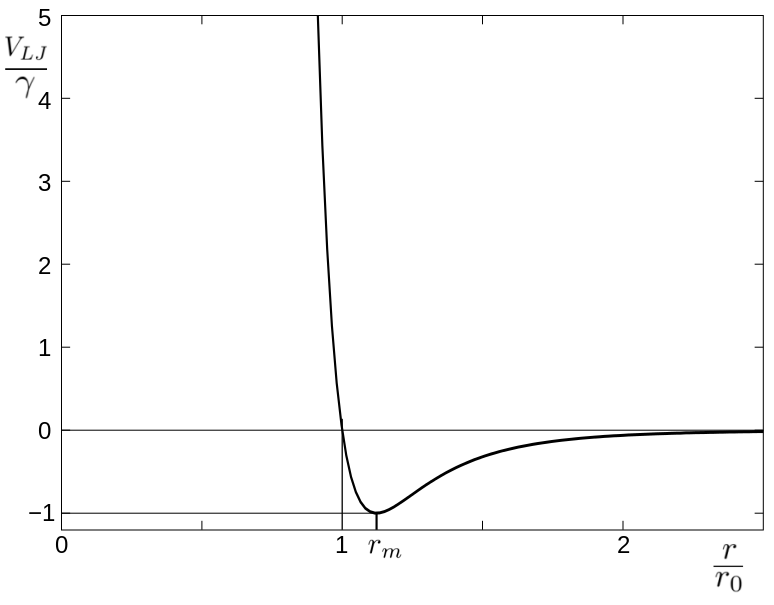
\includegraphics[width=10cm]{Cap_2/LJ.png}
\caption[Potencial de Lennard-Jones]{Gráfica del potencial Lennard-Jones normalizado a $\gamma$ y $r_{0}$}
\label{C2:fg:LJ}
\end{figure}

\subsection{Modelo de Átomo Embebido}
\label{SS2_3_2}

Este modelo es descrito en detalle en el trabajo de \cite{daw84}. En el mismo, la energía potencial es función de una suma de funciones de la separación entre un átomo y sus vecinos. La energía potencial de un átomo $i$ está dada por la \eref{C2:eq:EAM}:

\begin{equation}
V_{i} = F_{\alpha}\left(\sum_{i\neq j} \rho_{\beta} (r_{ij}) \right) + \frac{1}{2} \sum_{i\neq j} \phi_{\alpha\beta}(r_{ij})
\label{C2:eq:EAM}
\end{equation}

donde $r_{ij}$ es la distancia entre los átomos $i$ y $j$, $\phi_{\alpha\beta}$ es una función potencial entre pares de átomos, $\rho_{\beta}$ es la contribución a la densidad de carga electrónica del átomo $j$ de tipo $\beta$ en la ubicación del átomo $i$ y $F_{\alpha}$ es una función que representa la energía requerida para colocar el átomo $i$ de tipo $\alpha$ en la nube de electrones.

Al definir las funciones $\phi_{\alpha\beta}(r_{ij})$, $F_{\alpha}(\rho)$ y $\rho_{\beta} (r_{ij})$ se establece el modelo para un material en particular. En el caso de nuestras simulaciones, se tiene una aleación metálica de dos componentes, lo que implica definir siete funciones: tres funciones potenciales ($\phi_{\alpha\alpha}$, $\phi_{\alpha\beta}$, $\phi_{\beta\beta}$), dos funciones integradoras ($F_{\alpha}$, $F_{\beta}$) y dos funciones de contribución a la densidad de carga electrónica ($\rho_{\alpha}$, $\rho_{\beta}$).

Las funciones se encuentran en forma tabular en un archivo de formato \textit{setfl} \citep{setfl} que es leído por LAMMPS al indicarlo en el script de entrada. El archivo que utilizamos en nuestras simulaciones fue realizado por H.W.Sheng \citep{cheng09}.

%----------------------------------------------------------------------------------------
%	SECTION 4
%----------------------------------------------------------------------------------------
\section{Integración de las Ecuaciones de Movimiento}
\label{S2_4}

Existen diferentes algoritmos para la resolución numérica de las ecuaciones de movimiento de las partículas simuladas. En general, todos los métodos parten de la expansión en serie de Taylor de la posición y velocidad en función del tiempo. Esto, junto con la implementación computacional del algoritmo, hacen que siempre estén presentes dos errores: un error de truncamiento de la expansión en serie de Taylor, y un error de redondeo al usar un número finito de posiciones decimales.

Si bien los dos errores son inevitables, el error de truncamiento es propio del algoritmo y no podemos cambiar \textit{su orden}, mientras que el error de redondeo varía según la manera en que se haya implementado las operaciones matemáticas a nivel informático. Para $\Delta{}t$ grandes, predomina el error de truncamiento, mientras que para $\Delta{}t$ tendiendo a cero, predominan los errores de redondeo.

En este apartado describiremos los métodos \textbf{Verlet} (Sección \ref{S2_4_1}) y \textbf{Velocity Verlet} (Sección \ref{S2_4_2}). Este último es el usado por LAMMPS para nuestras simulaciones.

\subsection{Integración Verlet}
\label{S2_4_1}

Expandimos en primer lugar en serie de Taylor la posición para $t+\Delta{}t$ y $t-\Delta{}t$:
\vspace{-0.3pt}
\begin{align}
\mathbf{r}(t+\Delta{}t) & = \mathbf{r}(t)+\frac{d\mathbf{r}(t)}{dt} \Delta{}t + \frac{1}{2} \frac{d^{2}\mathbf{r}(t)}{dt^{2}} \Delta{}t^{2} + \frac{1}{3!} \frac{d^{3}\mathbf{r}(t)}{dt^{3}} \Delta{}t^{3} + \mathcal{O}(\Delta{}t^{4})
\label{C2:eq:VerletTaylor1} \\
\mathbf{r}(t-\Delta{}t) & = \mathbf{r}(t)-\frac{d\mathbf{r}(t)}{dt} \Delta{}t + \frac{1}{2} \frac{d^{2}\mathbf{r}(t)}{dt^{2}} \Delta{}t^{2} - \frac{1}{3!} \frac{d^{3}\mathbf{r}(t)}{dt^{3}} \Delta{}t^{3} + \mathcal{O}(\Delta{}t^{4})
\label{C2:eq:VerletTaylor2}
\end{align}

Sumando las Ecuaciones \ref{C2:eq:VerletTaylor1} y \ref{C2:eq:VerletTaylor2} y restando $\mathbf{r}(t-\Delta{}t)$ en ambos miembros obtenemos:

\begin{equation}
\mathbf{r}(t+\Delta{}t) = 2\mathbf{r}(t) - \mathbf{r}(t-\Delta{}t) + \frac{d^{2}\mathbf{r}(t)}{dt^{2}} \Delta{}t^{2} + \mathcal{O}(t^{4})
\label{C2:eq:VerletPos}
\end{equation}

La aceleración es calculada mediante el potencial visto anteriormente (\eref{C2:eq:potfza}) como:

\begin{equation}
\mathbf{a}(t) = \frac{d^{2}\mathbf{r}(t)}{dt^{2}} = -\frac{1}{m}\nabla{}V(\mathbf{r}(t))
\end{equation}

Una desventaja de este método es que las velocidades no se calculan directamente, y en general se obtienen de una aproximación por diferencias finitas centrales según:

\begin{equation}
\mathbf{v}(t) = \frac{\mathbf{r}(t+\Delta{}t) - \mathbf{r}(t-\Delta{}t)}{2\Delta{}t} + \mathcal{O}(t^{2})
\end{equation}

con lo cual el error deja de ser de $\mathcal{O}(\Delta{}t^{4})$ para ser de $\mathcal{O}(\Delta{}t^{2})$. Otro inconveniente es que para calcular las posiciones en un paso de tiempo, son necesarias las posiciones de dos pasos de tiempo atrás, por lo que el algoritmo requiere una inicialización de dos pasos. Esto último se resuelve en el método que se describe en el siguiente apartado.

\subsection{Integración Velocity Verlet}
\label{S2_4_2}

Partimos de la expansión en serie de Taylor de la posición y la velocidad en $t+\Delta{}t$:
\vspace{-0.3pt}
\begin{align}
\mathbf{r}(t+\Delta{}t) & = \mathbf{r}(t)+\frac{d\mathbf{r}(t)}{dt} \Delta{}t + \frac{1}{2} \frac{d^{2}\mathbf{r}(t)}{dt^{2}} \Delta{}t^{2} + \mathcal{O}(\Delta{}t^{3})
\label{C2:eq:VelVerletTaylor1} \\
\mathbf{v}(t+\Delta{}t) & = \mathbf{v}(t)+\mathbf{a}(t)\Delta{}t + \frac{1}{2}\frac{d\mathbf{a}(t)}{dt} \Delta{}t^{2} + \mathcal{O}(\Delta{}t^{3})
\label{C2:eq:VelVerletTaylor2}
\end{align}

La \eref{C2:eq:VelVerletTaylor2} puede reescribirse partiendo de la expansión en serie de Taylor de la aceleración:
\vspace{-0.3pt}
\begin{align}
\mathbf{a}(t+\Delta{}t) & = \mathbf{a}(t)+\frac{d\mathbf{a}(t)}{dt} \Delta{}t + \mathcal{O}(\Delta{}t^{2})
\label{C2:eq:tayloracc1} \\
\mathbf{a}(t)+\mathbf{a}(t+\Delta{}t) & = 2\mathbf{a}(t)+\frac{d\mathbf{a}(t)}{dt} \Delta{}t + \mathcal{O}(\Delta{}t^{2})
\label{C2:eq:tayloracc2} \\
\frac{1}{2}\Delta{}t\left[\mathbf{a}(t)+\mathbf{a}(t+\Delta{}t)\right] & = \mathbf{a}(t)\Delta{}t+\frac{1}{2}\frac{d\mathbf{a}(t)}{dt} \Delta{}t^{2} + \mathcal{O}(\Delta{}t^{3})
\label{C2:eq:tayloracc3}
\end{align}

Introduciendo la \eref{C2:eq:tayloracc3} en la \eref{C2:eq:VelVerletTaylor2}, obtenemos:

\begin{equation}
\mathbf{v}(t+\Delta{}t) = \mathbf{v}(t)+\frac{1}{2}\Delta{}t\left[\mathbf{a}(t)+\mathbf{a}(t+\Delta{}t)\right] + \mathcal{O}(\Delta{}t^{3})
\label{C2:eq:VelVerletTaylor3}
\end{equation}

Ahora podemos realizar la integración siguiendo los pasos a continuación:

\begin{enumerate}
	\item Calcular la velocidad en el paso de tiempo medio $t+\frac{\Delta{}t}{2}$
	\begin{equation}
	\mathbf{v}\left(t+\frac{\Delta{}t}{2}\right) = \mathbf{v}(t) + \frac{1}{2}\mathbf{a}(t)\Delta{}t
	\end{equation}
	\item Calcular las posiciones en el paso de tiempo $\Delta{}t$
	\begin{equation}
	\mathbf{r}(t+\Delta{}t) = \mathbf{r}(t) + \mathbf{v}\left(t+\frac{\Delta{}t}{2}\right)\Delta{}t
	\end{equation}
	\item Calcular las aceleraciones a partir del potencial
	\begin{equation}
	\mathbf{a}(t+\Delta{}t) = -\frac{1}{m}\nabla{}V\left(\mathbf{r}(t+\Delta{}t)\right)
	\end{equation}
	\item Actualizar las velocidades
	\begin{equation}
	\mathbf{v}(t+\Delta{}t) = \mathbf{v}\left(t+\frac{\Delta{}t}{2}\right) + \frac{1}{2}\mathbf{a}\left(t + \Delta{}t\right)\Delta{}t
	\end{equation}
\end{enumerate}

%----------------------------------------------------------------------------------------
%	SECTION 5
%----------------------------------------------------------------------------------------
\section{Termostatos y Barostatos}
\label{S2_5}

Si bien en las simulaciones básicas de MD se utiliza el ensamble microcanónico (NVE), para representar ciertos experimentos se necesita mantener constante otra variable que no sea la energía. Por ejemplo, una reacción química que se realiza en atmósfera libre sucede a presión constante y usamos el ensamble NPT; una reacción biológica puede ocurrir a temperatura constante y usaríamos el ensamble NVT.

Existen diversos métodos para mantener estos parámetros estables:

\begin{itemize}
	\item \textbf{Estocásticos}: Se obliga a una variable del sistema a seguir cierta distribución estadística.
	\item \textbf{De acoplamiento fuerte}: Se aplica una escala a una variable del sistema para llegar al valor exacto de la propiedad derivada.
	\item \textbf{De acoplamiento débil}: Se aplica una escala a una variable del sistema para establecer la tendencia de cambio hacia el valor deseado.
	\item \textbf{De extensión de la dinámica del sistema}: Se agregan grados de libertad adicionales.
\end{itemize}

Se explicará en el apartado siguiente un método usado en nuestras simulaciones para establecer la temperatura deseada mientras se simula con el ensamble NVE.

\subsection{Re-escalado de velocidades}
\label{S2_5_1}
Este método (en inglés \textit{velocity rescaling}) corresponde a un acoplamiento fuerte. Se calcula un factor $\lambda$ que multiplica a todas las velocidades de traslación del sistema. No se escalan las rotaciones. La temperatura del sistema se calcula según:

\begin{equation}
\sum_{i=1}^{N}\frac{m_{i}|\mathbf{v}_{i}|^{2}}{2} = \frac{k_{b}T}{2}(3N-N_{c})
\end{equation}

donde $k_{b}$ es la constante de Boltzmann, $\mathbf{v}_{i}$ las velocidades atómicas lineales, $m_{i}$ las masas atómicas, $T$ la temperatura, $N_{c}$ las restricciones y $3N-N_{c} = N_{gl}$ el número de grados de libertad. Entonces:

\begin{equation}
T = \sum_{i=1}^{N}\frac{m_{i}v_{i}^{2}}{N_{gl}k_{b}}
\end{equation}

Si multiplicamos las velocidades por un factor $\lambda$ para generar un salto $\Delta{}T$, calculamos $\lambda$ como sigue:

\begin{align}
\Delta{}T &= \sum_{i=1}^{N}\frac{m_{i}(\lambda{}v_{i})^{2}}{N_{gl}k_{b}} - \sum_{i=1}^{N}\frac{m_{i}v_{i}^{2}}{N_{gl}k_{b}}\\
T_{\tau} - T_{\tau{}-1} &= (\lambda{}^{2}-1)T_{\tau{}-1}\\
\frac{T_{\tau}}{T_{\tau{}-1}} - 1 &= \lambda{}^{2}-1 \\
\lambda{} &= \sqrt{\frac{T_{\tau{}}}{T_{\tau{}-1}}}
\end{align}

donde $T_{\tau{}-1}$ es la temperatura del paso de tiempo $\tau{}-1$ ya calculado y $T_{\tau}$ es la nueva temperatura.

\section{Scripting para pre y post-procesamiento}

\cambioGrande{TODA ESTA SECCION ES NUEVA !}

Para facilitar el procesamiento de datos, se desarrollaron diversos programas que de alguna manera asisten en las etapas presentes en un estudio atomístico. Podemos diferenciar por ejemplo:

\begin{itemize}
 \item Pre-procesamiento de la muestra
 \item Preparación del script de simulación en LAMMPS
 \item Secuenciación de tareas
 \item Generación de gráficas de calidad de publicación
 \item Análisis de Voronoi
\end{itemize}

Se explicará cada uno de estos puntos, y un detalle del código escrito puede encontrarse en el \aref{AD}.

\subsection{Pre-procesamiento de la muestra}

Como ejemplo de pre-procesamiento, se indica parte del código utilizado para colocar una esfera cristalina obtenida de un cristal prismático, dentro de una muestra de vidrio metálico.

\begin{enumerate}
 \item Extraer la cabecera de los archivos para que los mismos  comiencen con los datos de interés
 \item Extraer los identificadores de las partículas contenidas en la región esférica deseada \\
 \begin{lstlisting}
 awk -f extract_sphere_from_BMG Cu_Zr_160K.dat > SPHERE_IDS
  \end{lstlisting}
  siendo \lstinline[language=bash]|extract_sphere_from_BMG|:\\  
 \lstinputlisting[language=bash]{Scripts/extract_sphere_from_BMG}
 \item Extraer átomos de una esfera del mismo tamaño, del cristal prismático \\
  \begin{lstlisting}
 awk -f extract_sphere_from_B2_crystal CuZrB2Crystal.dat > SPHERE_ATOMS
  \end{lstlisting}
  siendo \lstinline[language=bash]|extract_sphere_from_B2_crystal|:\\  
  \lstinputlisting[language=bash]{Scripts/extract_sphere_from_B2_crystal}
  \item Reemplazar los átomos extraídos de la muestra original con los átomos del cristal \\
  \begin{lstlisting}
   python mix.py > NEW_ATOMS
  \end{lstlisting}
  (el detalle de \lstinline[language=bash]|mix.py| puede encontrarse en el \aref{AD} \sref{AD_Pub})
  %siendo \lstinline[language=bash]|mix.py|: \\
  %\lstinputlisting[language=Python]{Scripts/mix.py}
  \item Unir la muestra original sin los átomos de la región esférica extraída con los nuevos átomos \\  
  \begin{lstlisting}
   cat BMG_DATA_SPHERE_CUT > BMG_WITH_INCLUSION
   cat NEW_ATOMS >> BMG_WITH_INCLUSION
  \end{lstlisting}
  \item Agregar la cabecera correspondiente
\end{enumerate}


\subsection{Preparación del script de simulación en LAMMPS}

En cada simulación se deben indicar los diferentes parámetros que describen el experimento. Una lista no exhaustiva es presentada a continuación:

\begin{itemize}
 \item Unidades utilizadas
 \item Condiciones de borde (periódicas, no-periódicas)
 \item Tipo de átomo (indica los campos a leer y escribir en archivos)
 \item Átomos iniciales (lectura del archivo de la muestra)
 \item Masas de los diferentes átomos
 \item Datos de salida globales
 \item Datos de salida particulares
 \item Temperatura inicial
 \item Ensamble estadístico utilizado
 \item Paso de tiempo de cada paso de simulación
 \item Deformaciones aplicadas
\end{itemize}

Para los siete primeros puntos puede consultarse el \aref{AA}, donde se presenta de manera general los scripts de simulación y sus comandos. Ejemplos de la declaración de los cuatro últimos se pueden encontrar en el \aref{AD} \sref{AD_Sim}. Siempre se encuentra disponible el \href{http://lammps.sandia.gov/doc/Manual.html}{manual} de LAMMPS para ver en detalle la utilización de cada uno de los comandos.

\subsection{Secuenciación de tareas}

Al tener diversos casos de simulación (diferentes temperaturas, diferentes modos de carga, etc) se presenta la posibilidad de escribir códigos que permitan llevar adelante una cola de simulaciones programadas para no intervenir manualmente al finalizar cada una de ellas. Se desarrolla entonces un pequeño programa encargado de:

\begin{itemize}
 \item Iniciar automáticamente una simulación al agregar el comando de la misma en un archivo de texto.
 \item Reiniciar una simulación que se ha interrumpido.
 \item Escribir a un archivo \textit{log} el detalle de operaciones realizadas.
 \item Asignar nombres relevantes a los archivos de salida generados (según el último paso de tiempo).
\end{itemize}

El detalle de este código puede encontrarse en el \aref{AD} \sref{AD_Sec}.

\subsection{Generación de gráficas de calidad de publicación}

Como la presentación de resultados es una parte importante de toda investigación, se le dio importancia a la obtención de gráficos de buena calidad (\textit{publication ready} como se suele decir en inglés). Diversas herramientas fueron utilizadas, como \href{http://www.originlab.com}{Origin}, \href{https://www.r-project.org/}{R}, \href{http://www.gnuplot.info/}{Gnuplot} y \href{https://www.python.org/}{Python}. En el \aref{AD} \sref{AD_Pub} encontramos algunos ejemplos.

\subsection{Análisis de Voronoi}

Mediante Ovito \citep{stukowski10} pueden escribiste scripts en Python que automaticen diferentes análisis en un modo secuencial o \textit{pipeline}. En este trabajo se ha usado particularmente para estudiar la distribución de poliedros de Voronoi en las muestras a lo largo de la simulación. En el \aref{AB} se da una pequeña introducción a la utilización y en el \aref{AD} \sref{AD_Pub} se muestra un ejemplo completo. 
% Chapter Template

\chapter{CARACTERIZACION DE UN BMG BAJO DIFERENTES MODOS DE CARGA Y TEMPERATURAS} % Main chapter title

\label{C3} % Change X to a consecutive number; for referencing this chapter elsewhere, use \ref{ChapterX}

\lhead{Capítulo 3. \emph{CARACTERIZACION DE UN BMG}} % Change X to a consecutive number; this is for the header on each page - perhaps a shortened title

%----------------------------------------------------------------------------------------
%	SECTION 1
%----------------------------------------------------------------------------------------
%\section{Abstract}

%Amorphous metals, i.e. without defined crystal structure; are increasingly used in modern life, showing great potential as advanced engineering materials, due to some of its characteristic properties such as high hardness and moldability, high resilience, high mechanical strength and high wear resistance, among others. All these properties allow obtaining parts with complex shapes and high strength, which increases their chances for industrial application. However, many details of the mechanical behavior are still unknown, and the currently used models and theories are far from predictive.
%One of the possibilities to determine constitutive parameters, and thus study the response of these materials, is by using atomistic calculations. In this paper we present results obtained with molecular dynamics (MD) simulations, of an amorphous metal (CuZr). In particular, constitutive parameters such as elasticity modulus, are determined for samples at different temperatures and subjected to both tension and compression. The results obtained are relevant for understanding the mechanical behavior of the material, such as stress-strain and temperature-strain relationships. Additionally, it is possible to observe, under uniaxial tension, the nucleation and growth of a void due to high stress and strain rate values.

\section{Introducción}
\label{S3_1}

%Los materiales sólidos sin una estructura ordenada, es decir, amorfos, son llamados generalmente "vidrios". Algunos casos particulares de gran interés científico y tecnológico son los vidrios metálicos, que son aleaciones metálicas con propiedades mecánicas que sobrepasan en prestaciones a las aleaciones cristalinas más comunes (\cite{luborsky83}, \cite{greer95}). Se sabe que los metales forman fácilmente cristales cuando son enfriados (\cite{callister95}, \cite{smith96}). Sin embargo, usando una velocidad de enfriamiento suficientemente elevada y controlando la composición de la aleación, es posible obtener estructuras amorfas (\cite{liebermann93}), con la elasticidad de los polímeros y la resistencia de los metales (\cite{telford04}), teniendo también alta resistencia y moldeabilidad. Estas propiedades en su conjunto hacen posible la creación de partes de forma compleja y de alta resistencia, lo que además incrementa sus posibilidades de ser utilizados en aplicaciones industriales. Gracias a las propiedades citadas, estos materiales han sido de mucho interés como materiales estructurales en años recientes (\cite{chen74}, \cite{lowhaphandu99}, \cite{inoue00}, \cite{wang04}, \cite{ashby06}, \cite{zhang07}, \cite{schuh07}), incluyendo, por ejemplo, metales amorfos estructurales (\cite{lu04}), materiales biomédicos (\cite{zberg09}) o hasta incluso materiales aeroespaciales (\cite{peker93}), por nombrar algunos.

%Solid materials without an ordered structure, i.e. amorphous, are generally called "glasses". Particular cases of great scientific and technological interest are metallic glasses, which are metallic alloys with mechanical properties that outperform the most common crystalline alloys (\cite{luborsky83}, \cite{greer95}). It is known that metals easily form crystals when cooled (\cite{callister95}, \cite{smith96}). However, using a sufficiently fast cooling rate and controlling the composition of the alloy it is possible to obtain amorphous structures (\cite{liebermann93}), with the elasticity of polymers and the resistance of metals (\cite{telford04}), also having high strength and moldability. All these properties enable the creation of parts with complex shapes and high resistance, which further increases their chances of industrial applications. Thanks to the above properties, these materials have received great interest as structural materials in recent years (\cite{chen74}, \cite{lowhaphandu99}, \cite{inoue00}, \cite{wang04}, \cite{ashby06}, \cite{zhang07}, \cite{schuh07}), including, for example, amorphous structural steels (\cite{lu04}), biomedical materials (\cite{zberg09}) or even aerospace materials (\cite{peker93}), to name a few.

%Los vidrios metálicos son clasificados en general como vidrios metálicos convencionales o vidrios metálicos masivos (BMG) (\cite{wang04}, \cite{miller07}). Los BMG han sido recientemente empleados como fase matriz en materiales compuestos, mejorando varias de las propiedades originales de la fase dispersa como las propiedades mecánicas, magnéticas, etc. (\cite{telford04}, \cite{lu11}). En el caso particular de vidrios metálicos bajo deformación plástica, con la aparición de bandas de corte, de costumbre se abarca el problema con un enfoque en el comportamiento a nivel nano (\cite{ogata06}, \cite{guan10}), o mediante una aproximación usando mecánica del continuo (\cite{malvern69}).

%Metallic glasses can generally be classified as conventional metallic glasses or bulk metallic glasses (BMG) (\cite{wang04}, \cite{miller07}). BMG have recently been employed as matrix phase in composite materials, thus improving the various original properties of the dispersed phase such as mechanical, magnetic properties, etc. (\cite{telford04}, \cite{lu11}). In the particular case of metallic glasses under plastic strain, with the appearance of shear bands, it is customary to address the problem through a focus on nanoscale behavior (\cite{ogata06}, \cite{guan10}), or through an approach using continuum mechanics (\cite{malvern69}).

%Las simulaciones de dinámica molecular (MD) son usadas frecuentemente para estudiar propiedades a escala nano (\cite{allen87}). Las simulaciones de MD son una técnica muy poderosa que permite resolver, usando mecánica clásica, problemas con muchos cuerpos, dada una interacción entre átomos. Una ventaja de MD es que la deformación, el esfuerzo, la temperatura, la velocidad, etc. son todas conocidas en detalle (\cite{allen87}). Con esta información un gran número de fenómenos pueden estudiarse, como cambios de fase, transferencia de calor, creación y movimiento de dislocaciones, defectos, etc.. MD es una herramienta muy versátil para el estudio de las propiedades de materiales, y hasta ha sido utilizada para predecir el comportamiento mecánico de materiales previamente a los experimentos, como en el caso de maclas de aluminio (\cite{chen03}). Las simulaciones de MD reproducen el movimiento atómico y por lo tanto emplean pasos de tiempo de 1 fs (\cite{allen87}). Si modelamos una muestra hasta 10\% de deformación durante 1 millón de pasos de 1 fs, la velocidad de deformación será de $10^8$/s, que es adecuada para simular la deformación bajo láser de alta potencia, pero está lejos de serla para la mayoría de ensayos mecánicos en laboratorios. Como resultado, la extrapolación de resultados a bajas velocidades de deformación, debe realizarse cuidadosamente (\cite{bringa05}).

%Molecular dynamics (MD) simulations are often used to study nanoscale properties (\cite{allen87}). MD simulations are a very powerful technique that allows solving, using classical mechanics, problems with many bodies, given an interaction between atoms. One advantage of MD is that strain, stress, temperature, speed, etc. are all known in detail (\cite{allen87}). From this information large number of phenomena can be studied, such as phase changes, heat transfer, creation and movement of dislocations, defects, etc.. MD is a very versatile tool for studying the properties of materials, and has even been used to predict mechanical behavior of materials prior to  experiments, as in the case of aluminum twinned nanocrystals (\cite{chen03}). MD simulations reproduce the atomic motion and therefore employ time steps of 1 fs (\cite{allen87}). If modeling a sample up to 10\% strain during 1 million steps of 1 fs, the strain rate will be 108 /s, which is suitable for simulating deformation by high power lasers, but far from the majority of mechanical tests in laboratories. As a result, extrapolation to low strain rates has to be done carefully (\cite{bringa05}).

%Existen múltiples simulaciones de MD de metales amorfos. Las simulaciones de vidrios metálicos en particular se incrementaron por la presencia de potenciales de interacción adecuados para el sistema CuZr (\cite{ogata06}, \cite{arman10}, \cite{guan10}). En esta sección presentamos simulaciones de nivel atómico de un vidrio metálico CuZr sujeto a tracción y compresión, y analizamos sus respuestas como función de la temperatura.

%There are numerous molecular dynamics simulations of amorphous materials. The simulations of metallic glasses in particular have increased due to the presence of suitable interaction potentials for the CuZr system (\cite{ogata06}, \cite{arman10}, \cite{guan10}). In this paper we present atomic-scale simulations of CuZr metallic glasses subjected to tension and compression, and analyze their response as a function of their temperature.

%En esta sección presentamos simulaciones de nivel atómico (utilizando dinámica molecular) de un vidrio metálico CuZr sujeto a tracción y compresión, y analizamos sus respuestas como función de la temperatura.

La Ciencia de los Materiales cuenta con muchos experimentos que, a lo largo de los años, se han utilizado para conocer las propiedades mecánicas, térmicas, eléctricas, etc., de los materiales. Las propiedades mecánicas son, probablemente, las más estudiadas, debido a que en la mayoría de las situaciones los materiales se encontrarán bajo solicitaciones mecánicas, es decir, bajo la acción de fuerzas externas. Algunos de los ensayos más usuales son el ensayo de tracción, de compresión, de flexión, de fatiga, de dureza, etc..  

En este apartado se realizará un análisis del comportamiento mecánico de una muestra de vidrio metálico durante ensayos de tracción y compresión, a diferentes temperaturas. Primeramente, en la \sref{S3_2}, se detallarán los parámetros de las simulaciones. Luego, en la \sref{S3_3}, se mostrarán los resultados obtenidos a través de curvas y tablas para diferentes propiedades, tales como la relación tensión-deformación, el módulo de Young, la tensión máxima de Von Mises y la tensión de Von Mises a una determinada deformación.

\section{Detalles de las simulaciones}
\label{S3_2}
%In this paper, simulations were carried out using the LAMMPS software (\cite{plimpton95}), which is free and open source, has an excellent manual, and is computationally efficient in the simulation of systems with large numbers of atoms. 

Se utilizará, en el presente capítulo, una muestra de cobre-circonio. La muestra Cu$_{46}$Zr$_{54}$ usada es prismática, con un total de alrededor de 160000 átomos, creada con una velocidad de enfriamiento de $10^{12}$ K/s, y ya ha sido descrita por \cite{arman10}. La temperatura experimental de transición vítrea ($T_g$) de este vidrio metálico es 696 K, y su módulo de cizalla experimental (G) es 30 GPa \citep{johnson05}. Podemos observarla en la \fref{C3:fg:sample}. Se debe aclarar que así como en los metales se habla de \textit{probetas} para los ensayos mecánicos, en las simulaciones de vidrios metálicos se habla de \textit{muestras}. Esto se debe al tamaño \textit{nano} del material utilizado para la simulación (el término muestra suele utilizarse para denominar una pequeña parte de una cantidad mayor de material).

\begin{figure}
 \centering
 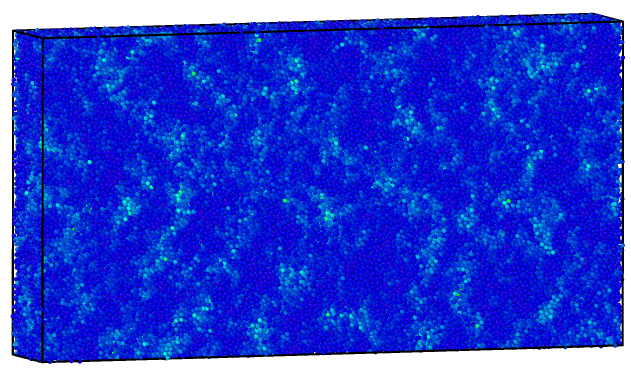
\includegraphics[width=10cm]{Cap_1/sample.png}
 \caption[Muestra utilizada en el trabajo]{Muestra Cu$_{46}$Zr$_{54}$ utilizada como base de las simulaciones de este trabajo.}
 \label{C3:fg:sample}
\end{figure}

Cada simulación diferirá de las restantes ya sea en el tipo de carga (tensión o compresión uniaxial) o en la temperatura de simulación, siendo constante la velocidad de deformación.

Se analizarán temperaturas de 10 (cercano al cero absoluto), 100, 200, 300, 400, 500, 600 y 900 K. Se incluye el caso de simulación a 900 K, sobre $T_g$, para ver si el comportamiento mecánico es significativamente diferente. Para describir las interacciones entre átomos, un potencial de método de átomo embebido (EAM) \citep{daw84} fue adoptado, que ya ha sido usado en otros estudios sobre BMGs \citep{shimizu07,cao09,cheng08,arman10,cheng11,wang12}.

En primer lugar se emplean condiciones de borde periódicas en 3D, válidas para altas velocidades de deformación \citep{bringa05}. Todas las coordenadas atómicas son escaladas a cada paso, de acuerdo con la velocidad de deformación deseada, que en este caso es de $10^9$ /s. Antes de iniciar las deformaciones mecánicas, se realiza primero una minimización de energía usando el gradiente conjugado, y luego usamos condiciones de presión cero y temperatura constante para equilibrar la muestra a la temperatura buscada T. La \tref{C3:tb:initprops} presenta los volúmenes y densidades iniciales para los diferentes casos.

%We use 3D periodic boundary conditions, suitable for high strain rates (\cite{bringa05}). All atomic coordinates are scaled every step, according to the desired strain rate, which in this case was 10$^{9}$ /s. Before starting mechanical strain simulations, we first perform energy minimization using conjugate gradient, and then use zero-pressure conditions and constant temperature to equilibrate the sample to the desired temperature T. Table 1 lists the volumes and initial sample densities for the different cases.

\begin{table}[htp]
\begin{center}
\begin{tabular}{*{3}{c}}
\hline
Temperatura [$K$] & Volumen [$nm^{3}$] & Densidad [$\frac{g}{cm^{3}}]$ \\ \hline \hline
10K & 2909.15 & 7.1705 \\ \hline
300K & 2931.93 & 7.1147 \\ \hline
600K & 2959.54 & 7.0484 \\ \hline
900K & 2992.30 & 6.9712 \\ \hline
\end{tabular}
\end{center}
\caption[Volúmenes y densidades iniciales]{Volúmenes y densidades iniciales a diferentes temperaturas simuladas.}
\label{C3:tb:initprops}
\end{table}

Luego, se analiza la presencia de bandas de corte para las condiciones de borde antes mencionadas. Por último, se investiga la respuesta frente a condiciones de borde no periódicas.

\section{Resultados}
\label{S3_3}

\subsection{Simulación de la muestra con condiciones de borde periódicas}
\label{S3_3_1}

En el texto que continúa, presentamos resultados para esfuerzos exclusivamente uniaxiales, los cuales son apropiados para la comparación con resultados de experimentos a una velocidad de deformación muy elevada, en donde las deformaciones laterales pueden despreciarse. 

La \fref{C3:fg:sStrainTen} grafica tensión de Von Mises versus deformación a todas las temperaturas simuladas. Luego de la deformación puramente elástica existe un decremento en la tensión de Von Mises, lo que sugiere la presencia de plasticidad. En la \fref{C3:fg:sStrain} se provee una estimación del fin del régimen elástico para poder observar mejor este fenómeno. Además, dadas la grandes velocidades de deformación y las grandes deformaciones, se nuclea un poro en la muestra bajo tracción, como vemos en la \fref{C3:fg:voidSeq}, lo cual produce grandes fluctuaciones de tensión luego de aproximadamente 15\% de deformación para $T=900K$, y luego de deformaciones un poco superiores para el resto de temperaturas.

%Below we present results for purely uniaxial strain, which is appropriate for the comparison with results of experiments at very high strain rates, where lateral strains can be neglected.
%Figure 1 (a) shows our results for von Mises stress versus strain at all the simulated temperatures. After the purely elastic deformation that occurs up to about 2\% strain, there is a decrease in von Mises tension, suggestive of plasticity. In addition, due to the high strain rates and large stress, there is a void nucleation in the sample under tension, as shown in Figure 2, which leads to large stress fluctuations after about 15\% strain.

\begin{figure}[htp]
\centering
\subfloat[Tracción]{
	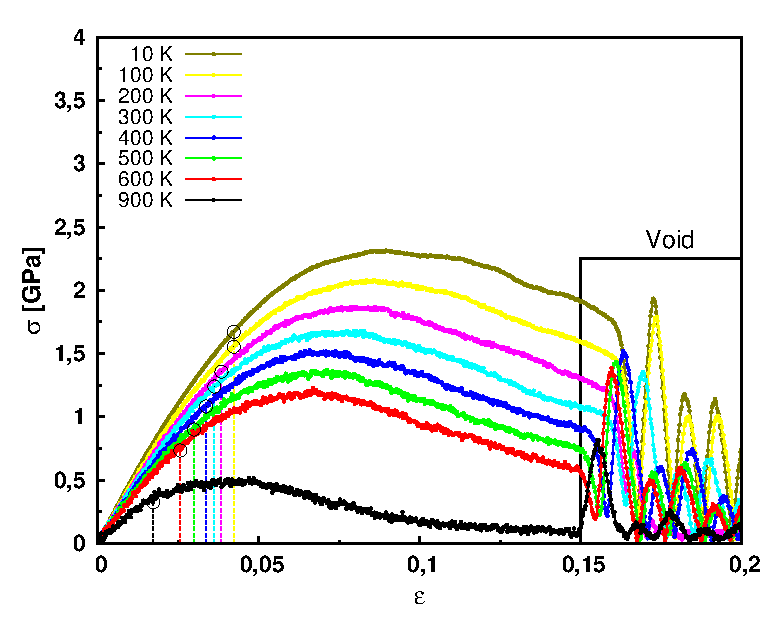
\includegraphics[width=8cm]{Cap_3/Tens_stress_strain_curve.eps}
	\label{C3:fg:sStrainTen}}
\subfloat[Compresión]{
	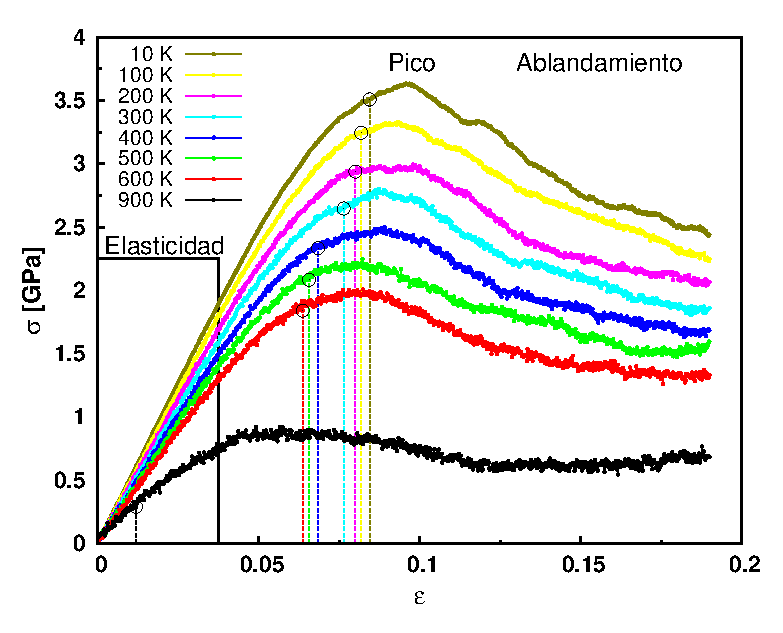
\includegraphics[width=8cm]{Cap_3/Comp_stress_strain_curve.eps}
	\label{C3:fg:sStrainComp}}
\caption[Curvas de tensión-deformación a diferentes temperaturas]{Curvas de tensión-deformación a diferentes temperaturas. Bajo tracción existen grandes fluctuaciones del esfuerzo que comienzan cuando se nuclea un poro a aproximadamente 15\% de deformación. Los círculos sobre las curvas denotan una estimación del fin de la deformación elástica, calculada como el punto donde la curva se aleja un 20\% del comportamiento elástico ideal.}
\label{C3:fg:sStrain}
\end{figure}

\begin{figure}[htp]
\centering
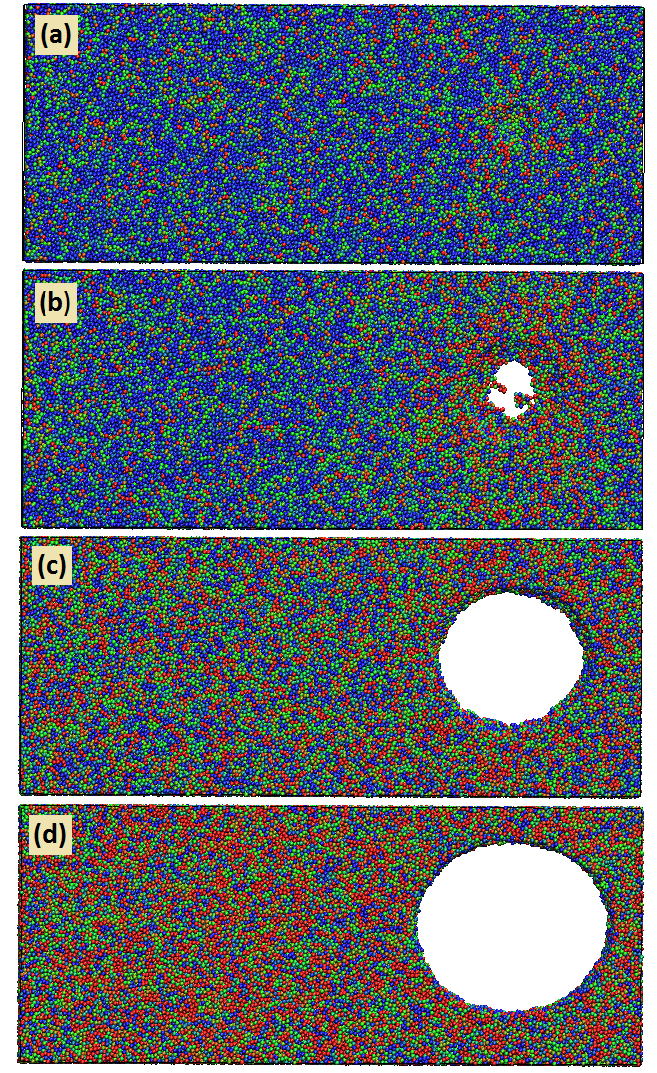
\includegraphics[width=10cm]{Cap_3/void_sequence.png}
\caption[Nucleación de un poro bajo tracción a 900 K.]{Nucleación de un poro bajo tracción a 900 K. (a) $\epsilon$ = 0.137 (b) $\epsilon$ = 0.141 (c) $\epsilon$ = 0.145 (d) $\epsilon$ =0.149. Los colores representan la tensión de Von Mises, rojo siendo alta tensión y azul baja tensión. Una nucleación similar es observada a temperaturas más bajas. ???}
\label{C3:fg:voidSeq}
\end{figure}

Calculamos las propiedades mecánicas y proponemos la siguiente forma funcional como aproximación del comportamiento térmico:

%We calculate mechanical properties, and propose the following simple functional form as an approximation for the thermal behavior:

\begin{eqnarray}
y = A_{1}\cdot \mathrm{e}^{\frac{-T}{T_{0}}}
\label{C3:eq:thermalFit}
\end{eqnarray}

donde $A_{1}$ y $T_{0}$ son parámetros. Esta forma funcional es frecuentemente usada para fenómenos activados térmicamente. En las Tablas \ref{C3:tb:initPropsTen} y \ref{C3:tb:initPropsComp} presentamos los valores para los coeficientes de la \eref{C3:eq:thermalFit} obtenidos de las curvas mostradas en las Figuras \ref{C3:fg:youngVsT} a \ref{C3:fg:peakVMises1218VsT}. Puede verse que las regresiones son razonables. El coeficiente de correlación ($R^2$) es mayor a 0.9 en todos los casos, haciendo razonable nuestra aproximación funcional simple.
	
%where $A_{1}$ and $T_{0}$ are parameters. This functional form is often used for thermally activated phenomena. In Tables 2-3 we present the values for the coefficients of equation (1) obtained from the curves shown in Figures 3-6. It can be seen that the fits are reasonable. The correlation coefficient (R2) is greater than 0.9 in all cases, thus making our simple functional fit reasonable. Of course, further studies including many more temperature values are needed to truly test the fits. 

\begin{table}[htp]
\begin{center}
\begin{tabular}{*{4}{c}}
\hline
\textbf{Tracción} & Parámetros & Valor & $R^{2}$ \\ \hline \hline
Peak Von Mises stress & A$_{1}$ & 2.29 $\pm$ 0.04 & 0.981 \\
 & T$_{0}$ & 1068.14 $\pm$ 68.02 & \\ \hline
Von Mises stress ($\epsilon$=0.12) & A$_{1}$ & 2.21 $\pm$ 0.02 & 0.998 \\
 & T$_{0}$ & 587.05 $\pm$ 13.45 & \\ \hline
Young Modulus & A$_{1}$ & 49.42 $\pm$ 0.38 & 0.990 \\
 & T$_{0}$ & 1924.38 $\pm$ 87.18 & \\ \hline
Yield Stress & A & 0.060 $\pm$ 0.002 & 0.972 \\
 & B & -0.037 $\pm$ 0.003 & \\ \hline
\end{tabular}
\end{center}
\caption[Coeficientes de la regresión para tracción]{Coeficientes de la regresión para tracción.}
\label{C3:tb:initPropsTen}
\end{table}

\begin{table}[htp]
\begin{center}
\begin{tabular}{*{4}{c}}
\hline
\textbf{Compresión} & Parámetros & Valor & $R^{2}$ \\ \hline \hline
Peak Von Mises stress & A$_{1}$ & 3.68 $\pm$ 0.03 & 0.997 \\
 & T$_{0}$ & 1020.16 $\pm$ 25.88 & \\ \hline
Von Mises stress ($\epsilon$=0.18) & A$_{1}$ & 2.64 $\pm$ 0.08 & 0.972 \\
 & T$_{0}$ & 824.98 $\pm$ 65.21 & \\ \hline
Young Modulus & A$_{1}$ & 52.22 $\pm$ 0.53 & 0.985 \\
 & T$_{0}$ & 1757.38 $\pm$ 96.61 & \\ \hline
Yield Stress & A & 0.125 $\pm$ 0.002 & 0.985 \\
 & B & -0.068 $\pm$ 0.003 & \\ \hline
\end{tabular}
\end{center}
\caption[Coeficientes de la regresión para compresión]{Coeficientes de la regresión para compresión.}
\label{C3:tb:initPropsComp}
\end{table}

Como es de esperarse, el módulo de elasticidad, la tensión máxima de Von Mises y la tensión de fluencia, todos decrecen con el aumento de la temperatura. Obtenemos un comportamiento suave incluso cuando T supera a $T_g$, como puede verse en las Figuras \ref{C3:fg:youngVsT} a \ref{C3:fg:peakVMises1218VsT}.

%As expected, the elastic modulus, peak von Mises stress and yield stress, all decrease with increasing temperature. We obtained a smooth behavior even when T is above $T_g$, as seen in Figures 3-6.

\begin{figure}[htp]
\centering
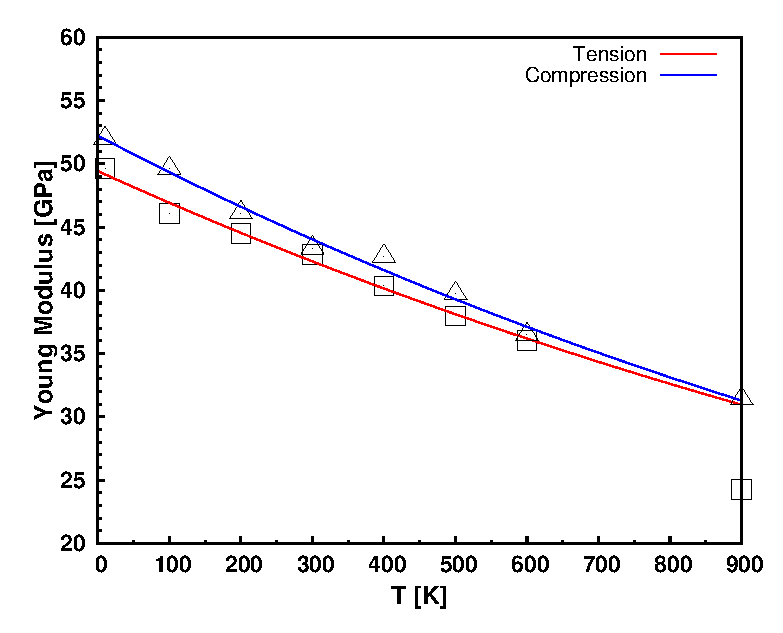
\includegraphics[width=10cm]{Cap_3/young_T_both.eps}
\caption[Aproximación módulo de Young-temperatura]{Aproximación módulo de Young-temperatura.}
\label{C3:fg:youngVsT}
\end{figure}

\begin{figure}[htp]
\centering
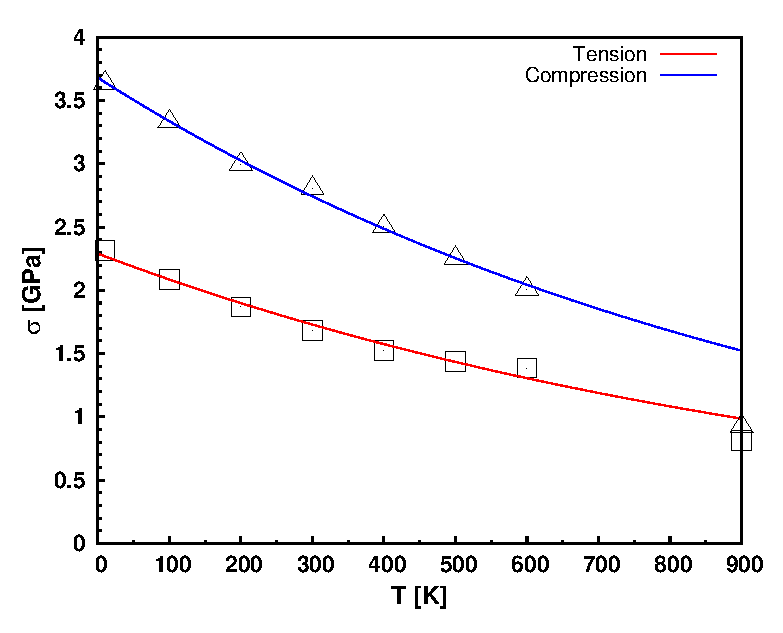
\includegraphics[width=10cm]{Cap_3/peakstress_T_BOTH.eps}
\caption[Aproximación tensión de Von Mises máxima-temperatura]{Aproximación tensión de Von Mises máxima-temperatura.}
\label{C3:fg:peakVMisesVsT}
\end{figure}

\begin{figure}[htp]
\centering
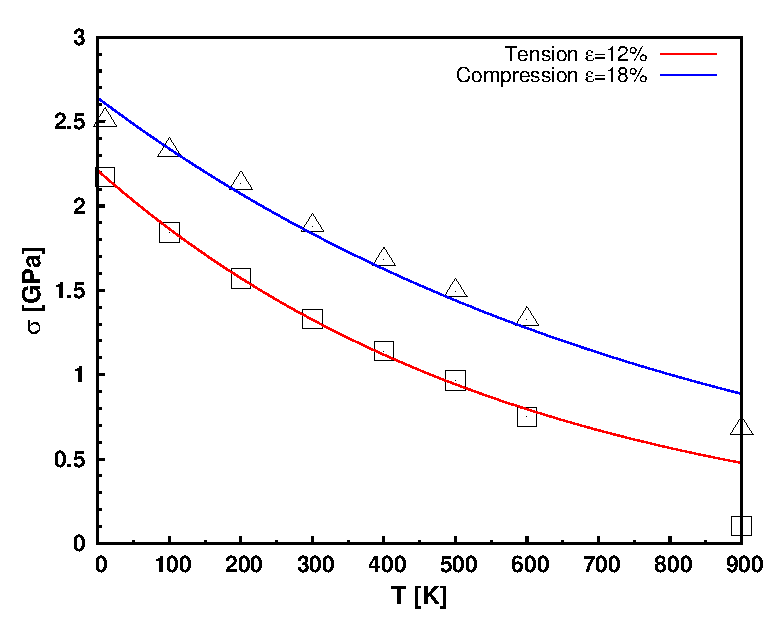
\includegraphics[width=10cm]{Cap_3/defstress_T_BOTH.eps}
\caption[Aproximación tensión de Von Mises-temperatura]{Aproximación tensión de Von Mises-temperatura. En tracción se utilizaron tensiones a deformaciones más bajas para evitar las fluctuaciones debidas a la nucleación del poro.}
\label{C3:fg:peakVMises1218VsT}
\end{figure} 

\cite{cheng11} buscó describir el comportamiento de una muestra sometida a esfuerzos cortantes puros al inicio de la plasticidad  como una función de algunas variables, incluyendo la temperatura, basándose en un CSM (modelo de corte cooperativo). Sus cálculos dieron una dependencia de la temperatura de la forma $(T/T_g)^{2/3}$. Tratamos de comparar este comportamiento con nuestros resultados. Simplificando la expresión en \cite{cheng11}, obtuvimos la siguiente expresión:

%\cite{cheng11} attempted to describe the behavior of the onset of plasticity under pure shear, as a function of several variables, including temperature, based on a CSM (cooperative shear model). The resulting temperature dependence was (T/$T_g$)2/3, and we try to apply this behavior to our results. Simplifying the expression in \cite{cheng11}, we obtain the following expression:

\begin{eqnarray}
\frac{\sigma{}_{y}}{G} = A+B\left( \frac{T}{T_g} \right)^{2/3}
\label{C3:eq:onsetPlast}
\end{eqnarray}

donde $\sigma{}_{y}$ es la tensión de fluencia, mientras que A y B son parámetros que se deben ajustar. Para obtener la tensión de fluencia en nuestras simulaciones utilizamos la siguiente regla: asumimos que la plasticidad comienza cuando la curva esfuerzo-deformación se aleja un 20\% del comportamiento elástico, el cual lo extrapolamos a partir de puntos obtenidos a deformaciones muy bajas (menores a $\epsilon$=1\%). En las Tablas \ref{C3:tb:initPropsTen} y \ref{C3:tb:initPropsComp} presentamos valores para los coeficientes de la \eref{C3:eq:onsetPlast} obtenidos para las curvas que se muestran en la \fref{C3:fg:fitDosTercios}. En esta figura comparamos las curvas ajustadas para tracción y compresión con el resultado de \cite{johnson05}, quien obtuvo, para  deformación cortante pura, la siguiente expresión:

%where $\sigma{}_{y}$ is the yielding stress, while A and B are parameters of the fit. To obtain the yield stress in our simulations we assume that plasticity starts when the stress-strain curve departs 20\% from the linear elastic behavior extrapolated from very low strains (below $\epsilon$=1\%). In Tables 2-3 we present the values for the coefficients of equation (2) obtained for the curves shown in Figure 6. In this figure we compare the fittings for tension and compression with the result from \cite{johnson05}, who obtained, for experiments under pure shear deformation the following expression:

\begin{eqnarray}
\frac{\tau _{y}}{G} = 0.036-0.016\left( \frac{T}{T_g} \right)^{0.62}
\label{C3:eq:johnsonSamwer}
\end{eqnarray}

donde $\tau _{y}$ es la tensión de fluencia cortante. Observamos que la \eref{C3:eq:onsetPlast} puede aproximar relativamente bien tanto la tracción como la compresión uniaxial. Hay ciertas discrepancias con la aproximación experimental de la \eref{C3:eq:johnsonSamwer}, pero notamos que los coeficientes de la aproximación tienen grandes márgenes de error, y los datos muestran mucha dispersión. Por ejemplo, el exponente es 0.62 $\pm$ 0.2.
	
%where $\tau _{y}$ is the shear yield strength .We observe that equation (2) fits both uniaxial tension and compression quite well. There are discrepancies with the experimental fit from equation (3), but we note that the coefficients in that fit had large error bars, and data showed large dispersion. For instance, the exponent was 0.62 $\pm$ 0.2.

\begin{figure}[htp]
\centering
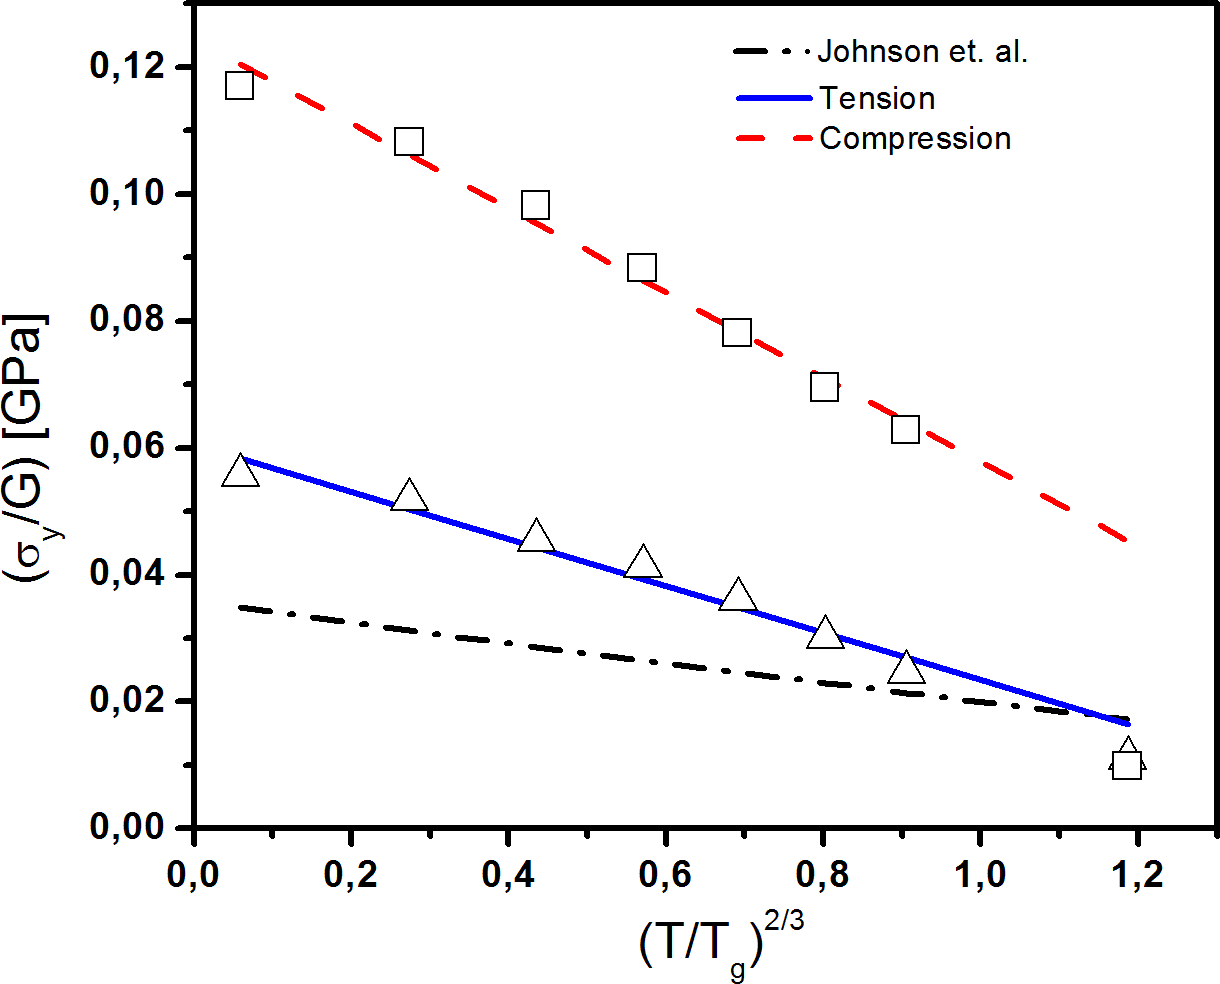
\includegraphics[width=10cm]{Cap_3/Fit2_Tercios.png}
\caption[Aproximación tensión de fluencia-temperatura]{Aproximación tensión de fluencia-temperatura. Utilizamos los valores experimentales de $T_g$ y G \citep{johnson05} para normalizar nuestros resultados.}
\label{C3:fg:fitDosTercios}
\end{figure}

La \fref{C3:fg:sampleTen} muestra la tensión de Von Mises a nivel atómico para la muestra completa (tracción a $T=300K$). A pesar de la evidencia de comportamiento plástico en las curvas esfuerzo-deformación, no observamos evidencia de bandas de corte.

%Figure 7 shows atomic von Mises stress for the complete sample in the case of tension at T=300K. Despite the evidence of plastic behavior in stress-strain curves, we do not observe evidence of shear bands.

De acuerdo a un estudio en nanocables de vidrio metálico \citep{xiao12}, la presencia de bandas de corte depende fuertemente de la velocidad de enfriamiento del vidrio. En este caso, para las velocidades de enfriamiento utilizadas en la creación de nuestra muestra, podría suceder que no se observen bandas de corte. Sin embargo, más adelante en esta sección se observarán posibles bandas de corte incipientes al graficar la deformación atómica en lugar de la tensión de Von Mises.

%According to a recent study in metallic glass nanowires (\cite{xiao12}), the presence of shear bands strongly depends on the quenching rate of the glass. In this case, for the quenching rates used in the creation of our sample, shear bands should not be observed, as shown in Figure 7.

\begin{figure}[htp]
\centering
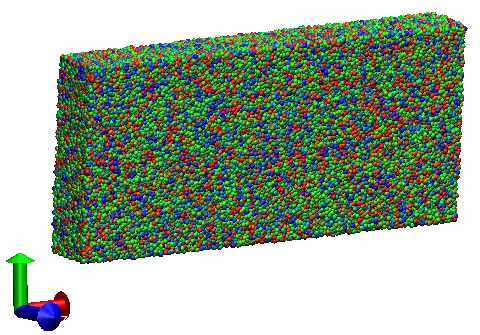
\includegraphics[width=10cm]{Cap_3/All_300K_6pstrain_sacale100-280_Trac.png}
\caption[Vista de la muestra a $\epsilon$=6\%, bajo tracción uniaxial, a T=300 K]{Vista de la muestra a $\epsilon$=6\%, bajo tracción uniaxial, a T=300 K. Los colores representan la tensión de Fon Mises. No se observan SB. La visualización fue realizada con VMD \citep{humphrey96}. Resultados similares se observan a otras temperaturas simuladas.}
\label{C3:fg:sampleTen}
\end{figure}

Cuando deformamos el vidrio metálico mediante compresión uniaxial podemos observar un comportamiento similar de las curvas esfuerzo-deformación mostradas en la \fref{C3:fg:sStrainComp} con respecto a las curvas de tracción mostradas en la \fref{C3:fg:sStrainTen}, siempre a deformaciones menores al 15\%. Luego del 15\% deformación las curvas de compresión tienen una forma suave debido a que no hay nucleación de poros.

%When the metallic glass deforms under uniaxial compression we can observe a similar behavior in the stress-strain curves shown in Figure 1 (b) to the curves corresponding to tension in Figure 1 (a), for strains below 15\%. However, since there is no void nucleation above 15\%, the behavior of the curves is smooth even at very high strains.

Las Figuras \ref{C3:fg:youngVsT} a \ref{C3:fg:fitDosTercios} muestran las mismas aproximaciones que las usadas para tracción. Las aproximaciones también son razonables, incluso con una ecuación de aproximación simple como la mostrada en la \eref{C3:eq:thermalFit}.

%Figures 3-6 show the same type of fit that the one used for tension, and there is also a reasonable adjustment, even with the simple functional form shown in equation (1).

La \fref{C3:fg:sampleComp} muestra que, de igual manera que en la muestra bajo tracción, no se observan bandas de corte.

%Figure 8 shows that, similarly to the sample under tension, no shear bands are observed, as expected given the high quenching rate of the glass used here.

\begin{figure}[htp]
\centering
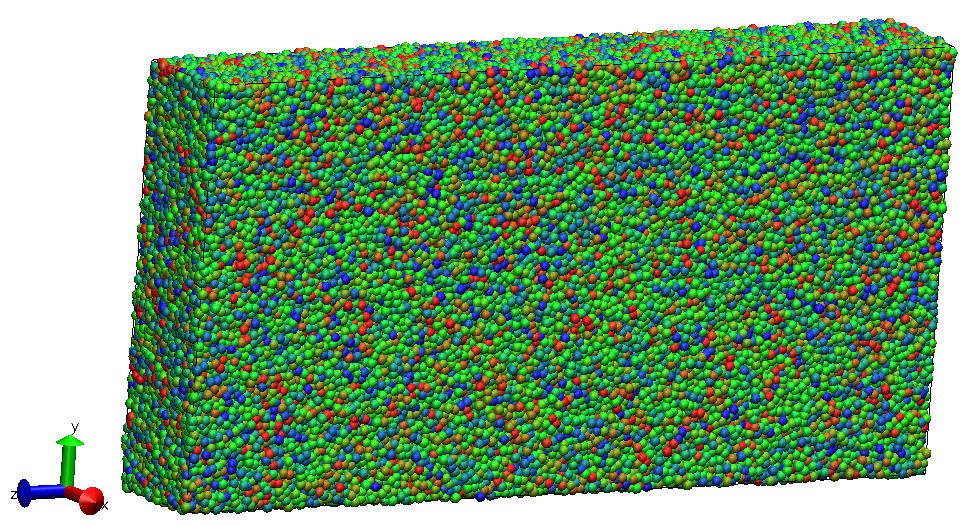
\includegraphics[width=10cm]{Cap_3/All_300K_6pstrain_sacale100-400_Comp.png}
\caption[Vista de la muestra a $\epsilon$=6\%, bajo compresión uniaxial, a T=300 K]{Vista de la muestra a $\epsilon$=6\%, bajo compresión uniaxial, a T=300 K. Los colores representan la tensión de Von Mises. No se observan SB. La visualización fue realizada con VMD \citep{humphrey96}. Resultados similares se observan a otras temperaturas simuladas.}
\label{C3:fg:sampleComp}
\end{figure}

Respecto a las bandas de corte, como se mencionó previamente, es posible observarlas graficando la deformación atómica de la muestra. Para esto se utiliza la herramienta Ovito, la cual utiliza el procedimiento descripto en \cite{shimizu07} para calcular la deformación atómica. La \fref{C3:fg:SBs} muestra el resultado.

\begin{figure}[htp]
\centering
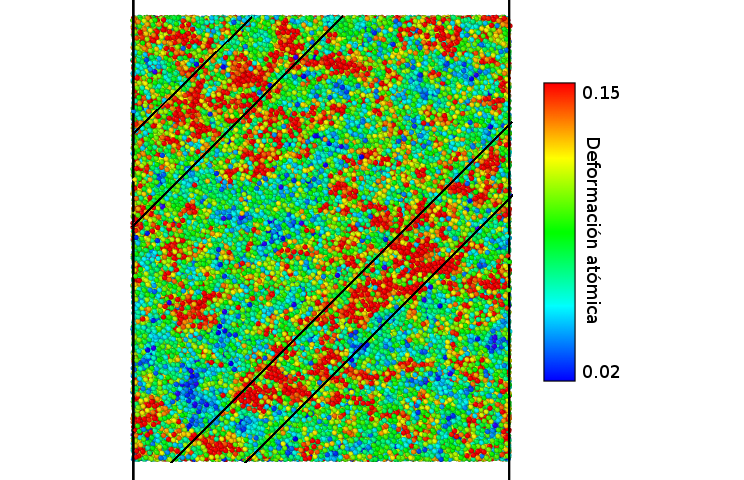
\includegraphics[width=10cm]{Cap_3/ShearBand.png}
\caption[Corte de la muestra a $\epsilon$=14\%, bajo compresión uniaxial, a T=300 K.]{Corte de la muestra a $\epsilon$=14\%, bajo compresión uniaxial, a T=300 K. Los colores representan la deformación atómica. La visualización fue realizada con Ovito \citep{stukowski10}. Se eliminan los efectos de la deformación homogénea para poder apreciar mejor la deformación heterogénea producto de las bandas de corte.}
\label{C3:fg:SBs}
\end{figure}

Es posible apreciar que las bandas de corte se forman con una dirección predominantemente diagonal, a prácticamente $45º$ con respecto a la dirección de aplicación de la fuerza. Las bandas de corte representan deformación heterogénea, lo cual puede llevar a la falla frágil del material. Esto es algo importante a tener en cuenta ya que puede reducir considerablemente la vida útil del material. En capítulos subsiguientes trataremos algunos métodos para retardar la propagación de bandas de corte.

\subsection{Simulación de la muestra con condiciones de frontera libres.}
\label{S3_3_2}

Para investigar la influencia de las condiciones de borde, se realizaron simulaciones con condiciones de frontera laterales libres, como se muestra en la \fref{C3:fg:libres}. Bajo tracción, \fref{C3:fg:libresTen}, hay una pequeña disminución de la sección transversal de la muestra, como era de esperar. Esto puede ser observado con mayor detalle en la \fref{C3:fg:cross}. También podemos observar que la forma de la sección transversal cambia de rectangular a elíptica, debido a un efecto de minimización de la energía de superficie.

%To verify that the absence of shear bands is not due to periodic conditions during deformation, simulations were carried out with free lateral boundary conditions, as shown in Figure 10. Under tension there is a slight decrease in the cross section of the sample, as expected. This is shown in Figure 11. We can also observe that the shape of the cross section has changed from rectangular to elliptical, due to surface energy minimization.

Estas simulaciones son similares a aquellas realizadas sobre nanocables de vidrio metálico en \cite{xiao12}. Bajo compresión, \fref{C3:fg:libresComp}, se observa pandeo. En ninguno de los casos se observan bandas de corte al graficar la tensión de Von Mises.

%These simulations are similar to those of metallic glass nanowires seen in \cite{xiao12}. Under compression, buckling is observed. In both cases there is a lack of shear bands, as expected with the cooling rates used in our samples.

\begin{figure}[htp]
\centering
\subfloat[Tracción]{
	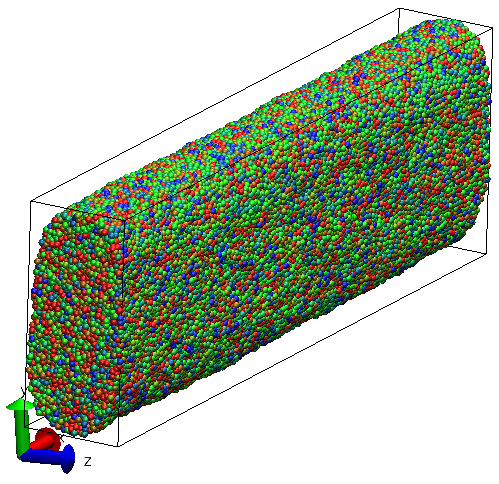
\includegraphics[width=8cm]{Cap_3/900libresTen.png}
	\label{C3:fg:libresTen}}
\subfloat[Compresión]{
	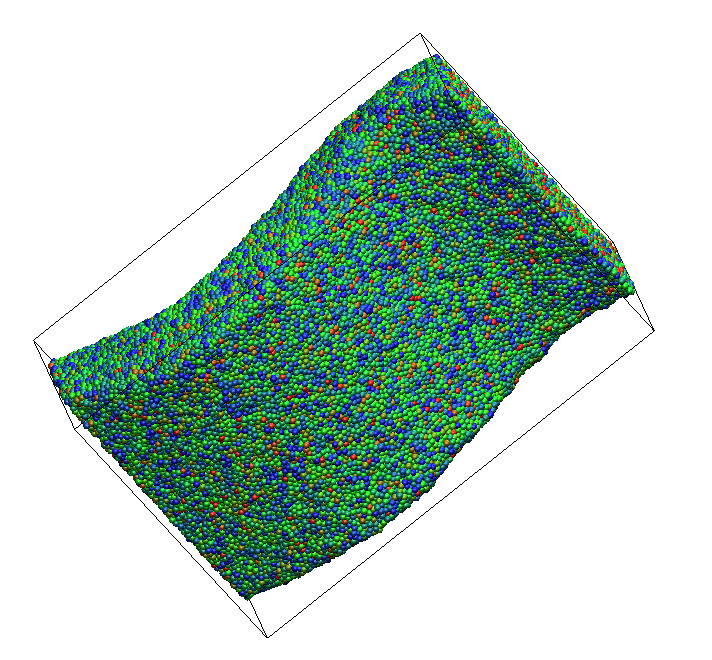
\includegraphics[width=8cm]{Cap_3/300libresComp.png}
	\label{C3:fg:libresComp}}
\caption[Simulaciones a tracción y compresión usando condiciones de frontera libres]{Simulaciones a tracción y compresión usando condiciones de frontera libres. En ambos casos $\epsilon$=0.20. En la muestra a tracción, T=900K, y T=300K a compresión. No se observa estricción en el caso a tracción, posiblemente debido a que la simulación se realizó a una temperatura superior a $T_g$. ???}
\label{C3:fg:libres}
\end{figure}

\begin{figure}[htp]
\centering
\subfloat[Sección próxima al extremo]{
	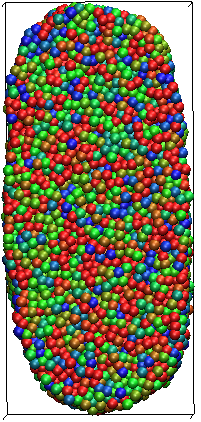
\includegraphics[width=3cm]{Cap_3/crossa.png}
	\label{C3:fg:crossExtreme}}
\subfloat[Sección central de la muestra]{
	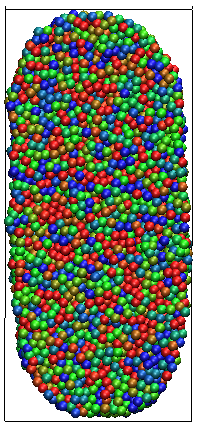
\includegraphics[width=3cm]{Cap_3/crossb.png}
	\label{C3:fg:crossMiddle}}
\caption[Sección transversal a diferentes distancias sobre el eje z usando condiciones de frontera libres]{Sección transversal a diferentes distancias sobre el eje z, para la simulación presentada en la \fref{C3:fg:libres}. No se aprecia estricción, incluso a altas deformaciones. ???}
\label{C3:fg:cross}
\end{figure}

%\section{Conclusiones}


%Atomistic simulations of bulk metallic glasses (BMGs) mechanical behavior under tension and compression were performed using molecular dynamics (MD) simulations. The increase of sample temperature produces a considerable decrease of the samples elastic modulus. The same applies to maximum von Mises stress. It is observed that the elastic modules are practically the same under tension or compression at different temperatures, but the maximum stress in compression is much higher. The behavior with temperature can be adjusted reasonably well with an exponential decay with temperature, typical of thermal activated phenomena.

%No shear bands are observed, which is to be expected given that our glass was generated with very high quenching rates. Since no shear bands are observed in our simulations, the identification of plasticity is complex. Surely there are shear areas, "shear transformation zones" (STZ), composed of a few atoms that experience high shear stresses. The identification of these areas requires a very detailed observation of the sample, involving much longer simulations than those used here. An alternative to study plasticity is the examination of Voronoi polyhedra, which can help to identify these areas. Such studies are in progress.

%In the future, using more powerful computational resources than available for this work, we plan to create samples with quenching rates orders of magnitude slower, with the aim to observe the possible formation of shear bands.

%A detailed understanding of the influence of temperature, quenching rates, etc., in the mechanical properties of metallic glasses will allow obtaining necessary properties for their application in new technologies, including applications under extreme conditions, such as aerospace missions or materials in nuclear reactors. Studies like the one presented here will contribute to this understanding and accelerate novel material development. 
% Chapter Template

\chapter{PROPIEDADES MECANICAS DE UN BMG CON NANOPARTICULAS CRISTALINAS EMBEBIDAS} % Main chapter title

\label{C4} % Change X to a consecutive number; for referencing this chapter elsewhere, use \ref{ChapterX}

\lhead{Capítulo 4. \emph{BMG CON NANOPARTICULAS CRISTALINAS EMBEBIDAS}} % Change X to a consecutive number; this is for the header on each page - perhaps a shortened title

\section{Introducción}
Al introducir nanopartículas a una matriz amorfa para mejorar las propiedades mecánicas (como se discute en el \cref{C1}) y asegurar efectos perdurables, las inclusiones deberían ser estables en el tiempo, es decir, no difundir en el material amorfo circundante perdiendo así la transición nítida entre cristal y amorfo.

En este apartado se analizan dos tipos de inclusiones cristalinas: nanopartículas de cobre cristalino con estructura de cubo centrada en las caras (Cu-FCC) y nanopartículas de cobre-circonio de fase B2 (CuZr-B2). Aunque no nos enfocamos en los efectos del tamaño de las inclusiones como otros estudios, se analiza la estabilidad de las nanopartículas a diferentes temperaturas. Durante la deformación mecánica de la muestra de un BMG con inclusiones bajo esfuerzo de tracción uniaxial, analizamos los poliedros de Voronoi y la distribución de esfuerzo y deformación cortante para estudiar el papel de la inclusión en las propiedades mecánicas de este material compuesto.

Primeramente, en la \sref{S4_2}, se estudia la estabilidad de la inclusión de CuZr (B2), ya que no es necesario estabilizar la fase antes de incrustar los átomos en la muestra, y esto no es posible directamente en LAMMPS. Luego, en la \sref{S4_3_1}, se muestran curvas de desplazamientos cuadráticos medios en función del tiempo para ambos sistemas, lo que da una idea de la estabilidad de la partícula en la matriz. Se presentan resultados tabulares de difusividad así como regresiones basadas en estos datos para mostrar la tendencia de comportamiento. En la \sref{S4_3_2} se presentan curvas de esfuerzo-deformación para diferentes temperaturas y ambos casos de inclusión cristalina.

%----------------------------------------------------------------------------------------
%	SECTION 1
%----------------------------------------------------------------------------------------

\section{Detalles de la Simulación}
\label{S4_1}

Analizamos inclusiones esféricas de cobre FCC. Una región de 2 nm de radio es eliminada de la muestra en una posición central, la cual fue luego llenada con la red cristalina correspondiente, es decir, una red cristalina FCC con una constante de red de 0.3615 nm. Luego de creados los átomos de Cu en la región esférica, la configuración fue minimizada, luego equilibrada a presión cero por algunos ps, luego calentada (o enfriada) para alcanzar la temperatura final deseada (\textit{T$_{f}$}) durante 4 ps y fue finalmente recocida y templada a \textit{T$_{f}$} por 1 ns.

En esta sección nos centramos en la estabilidad de las nanopartículas a diferentes temperaturas, aunque mostramos algunos casos de sometimiento a tracción y compresión uniaxial. Una velocidad de deformación homogénea de 10$^{9}$/s es aplicada. La Difusividad en todos los casos se calcula ajustando los desplazamientos cuadráticos medios (en inglés \textit{Mean Squared Displacements} o MSD) $\langle r^{2}\rangle$, obtenidos de LAMMPS.

\section{Creación de un cristal de CuZr de fase B2}
\label{S4_2}

Para incrustar estas partículas es necesario reemplazar átomos de la muestra original (estudiada en el \cref{C3}) por átomos ordenados del material buscado. LAMMPS permite el llenado directo de una región con estructura FCC, pero no así con fase B2. Es por eso que es necesario  primero crear una pequeña muestra con la estructura buscada de donde tomar el grupo de átomos necesario (en este caso, una esfera) y colocarlo en una región del mismo tamaño en la muestra original.

Creamos para esto un cubo cristalino aislado de 15 celdas unitarias de ancho para verificar el procedimiento, con una constante de celda de 3.50 \AA{}, tomado según \cite{inoue04}. En este paso se utilizan condiciones de borde periódicas en las tres direcciones. Se realiza un proceso de minimizado de energía y relajación a presión cero. Se crean las velocidades iniciales para lograr una temperatura de 1100 K (\textit{T$_{B2}$}), según \cite{pauly10}, quien indica una temperatura de fase B2 estable entre 988 K y 1200 K. 

Se equilibra la muestra a presión cero y \textit{T$_{B2}$} en 100 ps, seguido de un recocido a \textit{T$_{B2}$} por 150 ps para ser enfriada rápidamente a 300 K a 10$^{12}$ K/s para igualar la velocidad de enfriamiento de la matriz. Los parámetros de la estructura obtenida se muestran en la \tref{C4:tb:b2CrystalParameters}.
%We first create an isolated small cubic crystal of 15 lattices wide to verify the procedure with an initial lattice constant of 3.50 \AA{}, according to \cite{inoue04}. Periodic boundaries in all directions are used in this step. This crystal is then minimized and relaxed at zero pressure. Initial velocities are created for a temperature of 1100 K (\textit{T$_{B2}$}), according to \cite{pauly10} who indicates B2 stable phase temperature between 988 K and 1200 K.
%Equilibration to zero pressure is then performed at \textit{T$_{B2}$} in 100 ps, followed by annealing at \textit{T$_{B2}$} for 150 ps and a quenching to 300 K at 10$^{12}$ K/s to match sample quenching rate. Final parameters of the created structure are shown in Table \ref{table:b2CrystalParameters}.

\begin{table}[htp]
\begin{center}
\begin{tabular}{*{2}{c}}
\hline
Velocidad de enfriamiento [K/s] & 10$^{12}$ \\
\hline
Número de átomos & 6750 \\
\hline
Constante de celda [\AA] & 3.283 \\
\hline
Energía total (eV) & -34012.8 \\
\hline
Energía de cohesión (eV) & -5.04 \\
\hline
\end{tabular}
\end{center}
\caption{Parámetros obtenidos para el cristal CuZr (B2)}
\label{C4:tb:b2CrystalParameters}
\end{table}

Luego realizamos un recocido de 100 ps a 300 K utilizando el ensamble $NVE$ de una esfera de 2 nm extraída del cristal obtenido. La \fref{C4:fg:B2Crystal} muestra el cristal resultante y la \fref{C4:fg:B2CrystalTest} muestra la evolución de la energía de cohesión en el tiempo. Es posible que la pendiente negativa en los primeros 20 ps a 25 ps sea consecuencia de una elección no óptima de la densidad inicial del cristal. Al observar que la energía se conserva en el tiempo, concluimos que la partícula así formada es estable y puede incluirse en la matriz de BMG.

%We then run a 100 ps annealing at 300 K with nve time integration of a 2 nm radius sphere cutted off the obtained cluster.
%Fgure \ref{figure:B2CuZr_Formation} \subref{figure:B2Crystal} shows the resulting crystal and figure \ref{figure:B2CuZr_Formation} \subref{figure:B2CrystalTest} shows the evolution of cohesive energy in time. The negative slope in the firsts 20-25 ps may be consequence of a not optimal initial density of the cluster. We observe that the energy is conserved and we conclude this cluster is stable to be included in the BMG sample.

\begin{figure}[htp]
\centering
\subfloat[Cristal resultante de CuZr (B2) (corte en imagen inferior)]{
	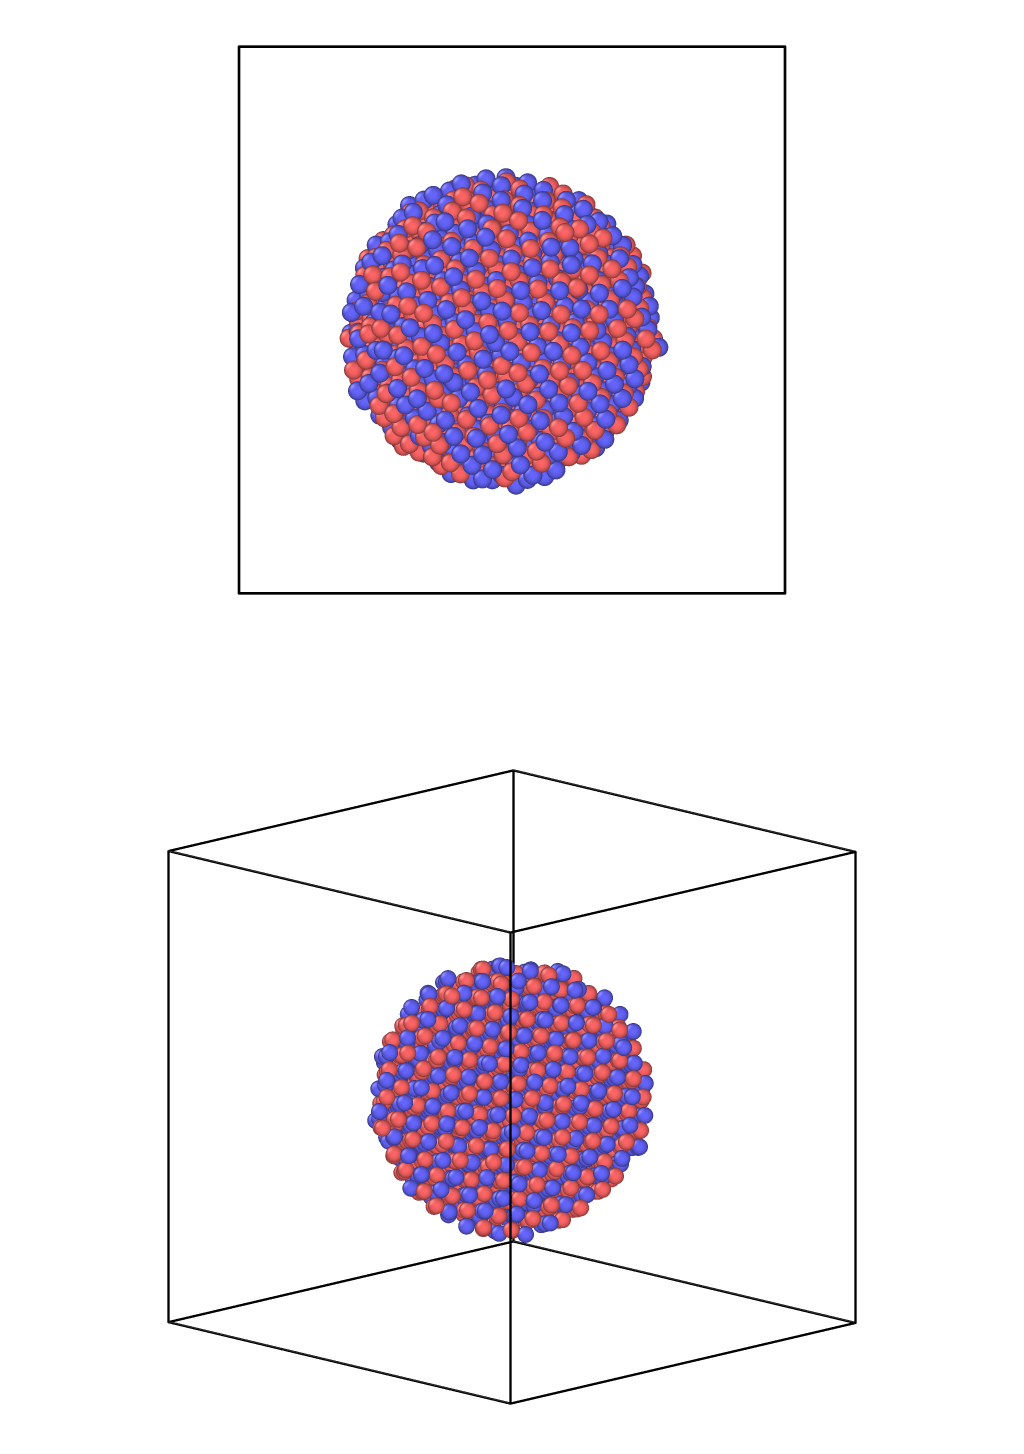
\includegraphics[width=5cm]{Cap_4/B2_FreeBoundaries.png}
	\label{C4:fg:B2Crystal}}
\quad
\subfloat[Energía de cohesión vs tiempo para el cristal de CuZr (B2) generado]{
	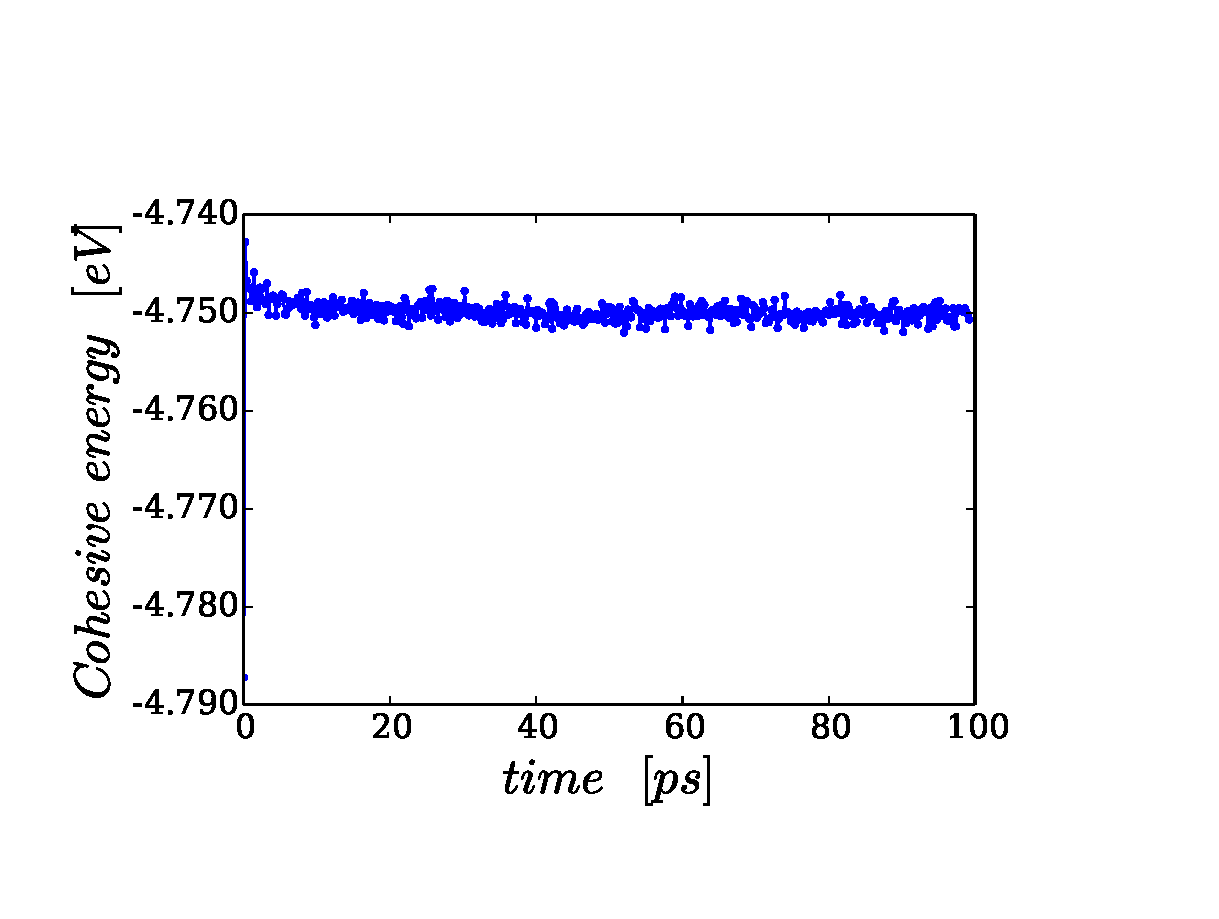
\includegraphics[width=10cm]{Cap_4/B2CrystalTest_FreeBoundariesSphere.pdf}
	\label{C4:fg:B2CrystalTest}}
\caption{Formación del cristal CuZr (B2)}
\label{C4:fg:B2CuZr_Formation}
\end{figure}

%After obtaining the initial-step configuration with this inclusion, we heat (or cool) the sample to \textit{T$_{f}$} and run an annealing for $1\,ns$, like we did with FCC-Copper inclusions.

\section{Resultados}
\label{S4_3}

En esta sección analizamos la estabilidad de nanopartículas a diferentes temperaturas, hasta temperaturas cercanas a la transición vítrea. En una primer parte, se presentan los resultados de la estabilidad de la nanopartícula y la difusividad calculada. Para tener un mismo parámetro de comparación, se utilizan los resultados obtenidos para la inclusión de Cu-FCC. Se eligen con esa información el rango de temperaturas y la ventana de tiempo tenida en cuenta. Luego se presenta la respuesta de la muestra ante esfuerzos de carga uniaxiales tanto de tracción como de compresión.

\subsection{Estabilidad de la Inclusión}
\label{S4_3_1}

La información obtenida de los MSD para los átomos de la inclusión se obtienen de simulaciones a diferentes temperaturas. Como podemos ver en la \fref{C4:fg:msd10_400_FCC}, para la nanopartícula de Cu-FCC, luego de un transitorio inicial los MSD se vuelven casi constantes, conduciendo a una difusividad cercana a cero, como es de esperar para una inclusión solida estable.

Esto indicaría que las inclusiones de Cu-FCC son de hecho estables en condiciones de operación normal para BMGs. Sin embargo, las simulaciones de MD cubren en general un corto periodo de tiempo de sólo algunos ns, y nos centramos ahora en temperaturas más elevadas para una mejor evaluación de la estabilidad de la nanopartícula. Elegimos entonces el rango de temperaturas para T $ \geq 500$ K (tanto para el caso de Cu-FCC como para el caso de CuZr-B2).

Los datos de MSD representan una media de todos los átomos de la nanopartícula, pero podrían existir grandes diferencias entre los átomos del núcleo y la superficie de la inclusión. Es por ésto que calculamos los MSD de los átomos de Cu en una región de corona esférica de un espesor de 0.8 nm y radio interno de 1.2 nm. Puede verse en la \fref{C4:fg:FCCdiff_shell_comp} que, luego de un transitorio de unos 0.6 ns, las pendientes de los MSD son prácticamente iguales para la corona y la nanopartícula en su totalidad. Elegimos entonces la ventana temporal para t $ \geq 0.6 $ ns.

Las curvas de MSD para el caso de Cu-FCC se ven entonces en las Figuras \ref{C4:fg:msd10_400_FCC} y \ref{C4:fg:msd500_800_FCC} y para el caso de CuZr-B2 en las Figuras \ref{C4:fg:msd10_400_B2} y \ref{C4:fg:msd500_800_B2}.

Obtenemos entonces para T $ \geq 500$ K y t $ \geq 0.6 $ ns las difusividades que se muestran en las Tablas \ref{C4:tb:FCC_Diff_Fit_Restults} y \ref{C4:tb:B2_Diff_Fit_Restults}, usando la ecuación de Einstein $\langle r^{2}\rangle = 6Dt$.

Las difusividades son ajustadas para tener correspondencia con la ecuación \ref{C4:eq:diff_Fit}, donde $k_{B}$ es la constante de Boltzmann, $\Delta E$ es la energía de activación para difusión, y $D_{0}$ da la escala de difusividad. La regresión resultante aparece en la \tref{C4:tb:FCC_Diff_VS_T_Fit_Restults} y son mostrados gráficamente en la \fref{C4:fg:FCC_diff_vs_T}. Hay que considerar que al ser tan bajos los valores obtenidos para el caso de CuZr-B2, esta regresión sólo se calcula para el caso Cu-FCC.

Es de notar que si bien las difusividades para el caso de CuZr-B2 son mucho menores (la pendiente de los movimientos atómicos es cercana a cero), el desplazamiento inicial de los átomos durante el calentamiento a la temperatura de simulación (por ejemplo desde 300 K a 500 K) es mucho mayor. En las Figuras \ref{C4:fg:heating500_800_FCC} y \ref{C4:fg:heating500_800_B2} observamos esto claramente.

Por último, como fue señalado en \cite{albe13}, el núcleo de las inclusiones se ve reducido porque los átomos más externos tienden a volverse amorfos. Este efecto se incrementa con la temperatura, como era de esperarse, cuando la difusión atómica es mayor.

\begin{figure}[htp]
\centering
\subfloat[Bajas temperaturas]{
	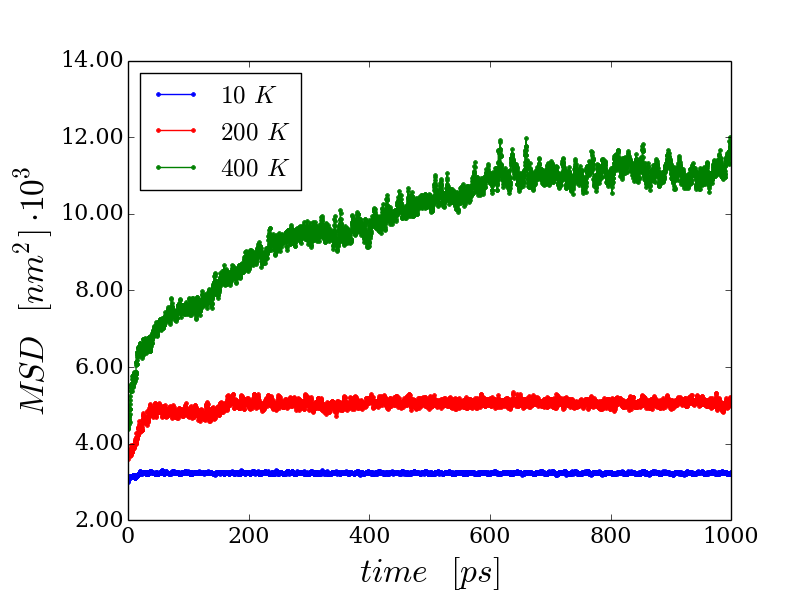
\includegraphics[width=10cm]{Cap_4/msd10_400_FCC.png}
	\label{C4:fg:msd10_400_FCC}}
\\
\subfloat[Altas temperaturas]{
	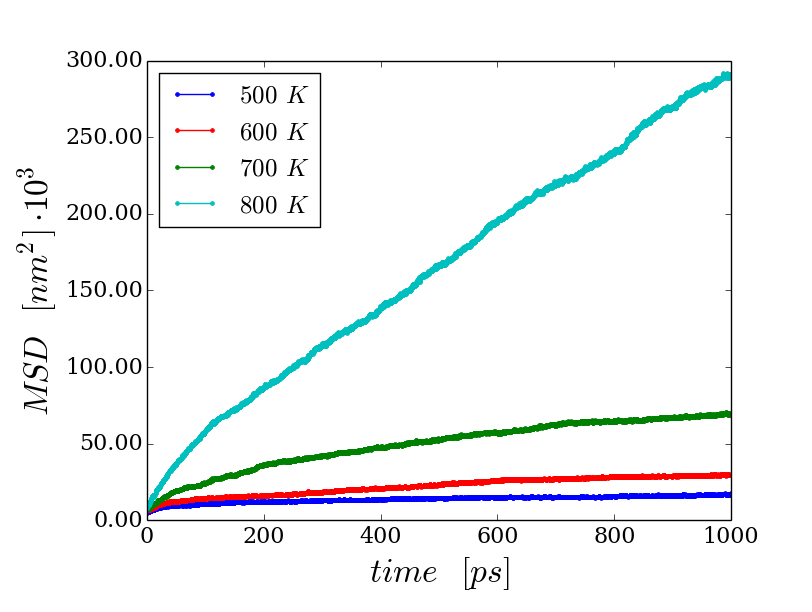
\includegraphics[width=10cm]{Cap_4/msd500_800_FCC.png}
	\label{C4:fg:msd500_800_FCC}}
\caption[MSD para inclusión de Cu FCC a diferentes temperaturas]{MSD para inclusión de Cu FCC a diferentes temperaturas}
\label{C4:fg:msd_Cu_FCC}
\end{figure}

\begin{figure}[htp]
\centering
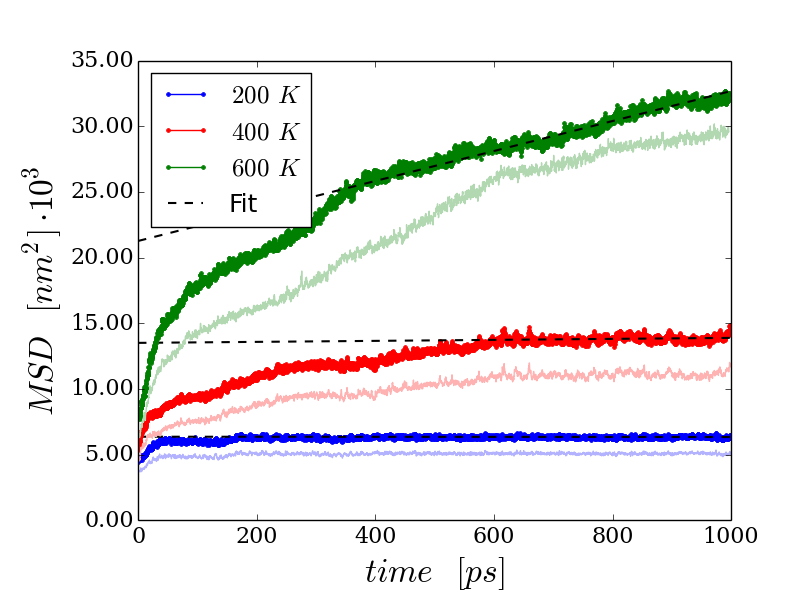
\includegraphics[width=10cm]{Cap_4/FCCdiff_shell_comp.png}
\caption[MSD de la corona esférica y la nanopartícula completa]{MSD de la corona esférica y para la nanopartícula completa (color más claro)}
\label{C4:fg:FCCdiff_shell_comp}
\end{figure}

\begin{table}[htp]
\begin{center}
\begin{tabular}{*{3}{c}}
\hline
T [$K$] & D [$\frac{nm^{2}}{ps}$] & R$^{2}$ \\
\hline \hline
500 & $8,490\cdot 10^{-7}$ & 0,8306 \\
\hline
600 & $1,508\cdot 10^{-6}$ & 0,9253 \\
\hline
700 & $4,699\cdot 10^{-6}$ & 0,9357 \\
\hline
800 & $4,149\cdot 10^{-5}$ & 0,9935 \\
\hline
\end{tabular}
\end{center}
\caption{Resultados del ajuste de la difusividad para el caso Cu-FCC}
\label{C4:tb:FCC_Diff_Fit_Restults}
\end{table}

\begin{figure}[htp]
\centering
\subfloat[Bajas temperaturas]{
	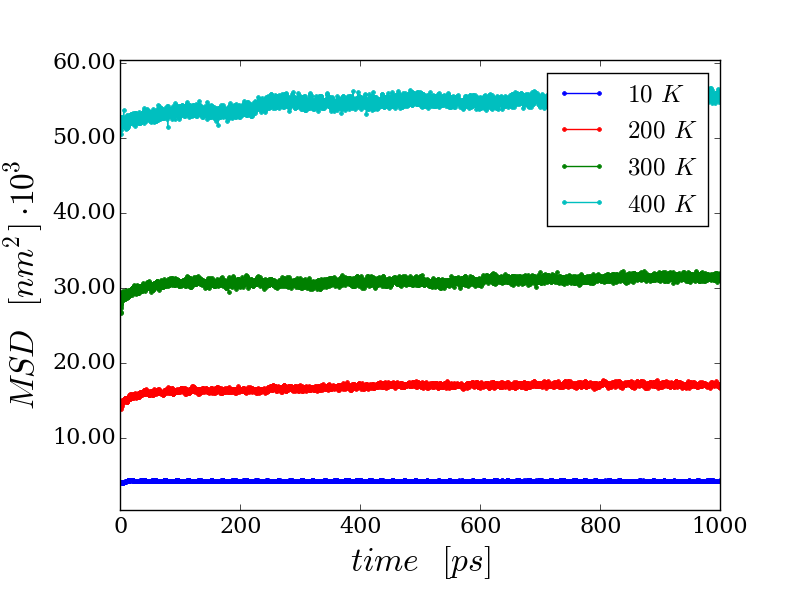
\includegraphics[width=10cm]{Cap_4/msd10_400_B2.png}
	\label{C4:fg:msd10_400_B2}}
\\
\subfloat[Altas temperaturas]{
	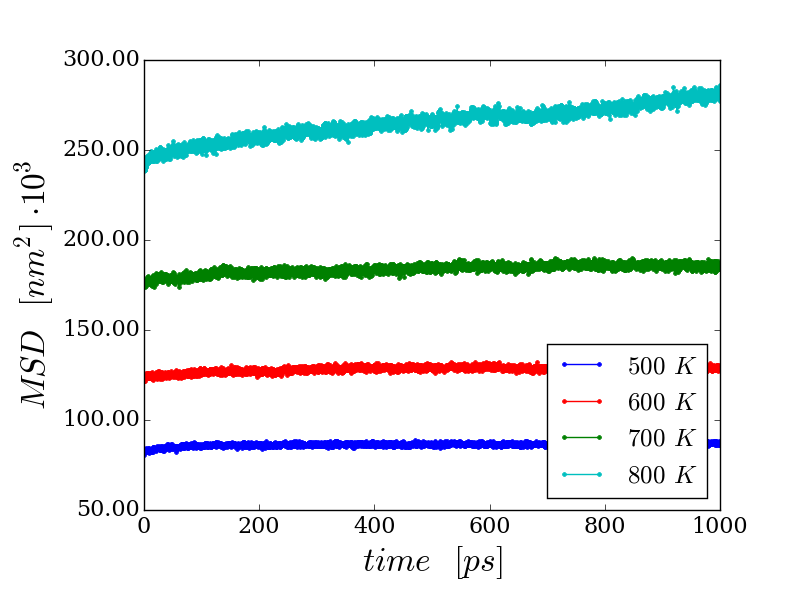
\includegraphics[width=10cm]{Cap_4/msd500_800_B2.png}
	\label{C4:fg:msd500_800_B2}}
\caption[MSD para inclusión de CuZr B2 a diferentes temperaturas]{MSD para inclusión de CuZr B2 a diferentes temperaturas}
\label{C4:fg:msd_CuZr_B2}
\end{figure}

\begin{table}[htp]
\begin{center}
\begin{tabular}{*{3}{c}}
\hline
T [$K$] & D [$\frac{nm^{2}}{ps}$] & R$^{2}$ \\
\hline \hline
500 & $2,104\cdot 10^{-7}$ & 0,0452 \\
\hline
600 & $7,094\cdot 10^{-8}$ & 0,0026 \\
\hline
700 & $2,122\cdot 10^{-7}$ & 0,0112 \\
\hline
800 & $5,712\cdot 10^{-6}$ & 0,7940 \\
\hline
\end{tabular}
\end{center}
\caption{Resultados del ajuste de la difusividad para el caso CuZr-B2}
\label{C4:tb:B2_Diff_Fit_Restults}
\end{table}

\begin{eqnarray}
D = D_{0}\cdot \mathrm{e}^{\frac{-\Delta E}{k_{B} T}}
\label{C4:eq:diff_Fit}
\end{eqnarray}

\begin{figure}[htp]
\centering
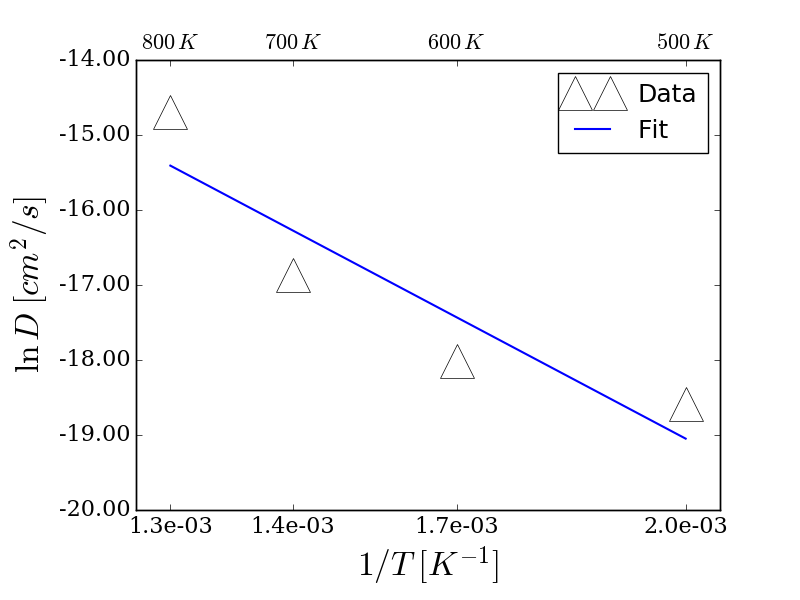
\includegraphics[width=10cm]{Cap_4/FCCDiff_vs_temp_fit.png}
\caption[Difusividad en función de la temperatura (Cu-FCC)]{Difusividad en función de la temperatura para el caso Cu-FCC}
\label{C4:fg:FCC_diff_vs_T}
\end{figure}

\begin{table}[htp]
\begin{center}
\begin{tabular}{*{2}{c}}
\hline
Energía de activación [$eV$]& $-0,4182$ \\
\hline \hline
D$_{0}$ [$\frac{nm^{2}}{ps}$] & $8,771\times 10^{-3}$\\
\hline
R$^{2}$ & 0.8399 \\
\hline
\end{tabular}
\end{center}
\caption{Resultados del ajuste de la difusividad con respecto a la temperatura (inclusión de Cu-FCC)}
\label{C4:tb:FCC_Diff_VS_T_Fit_Restults}
\end{table}

\begin{figure}[htp]
\centering
\subfloat[Nanopartícula Cu-FCC]{
	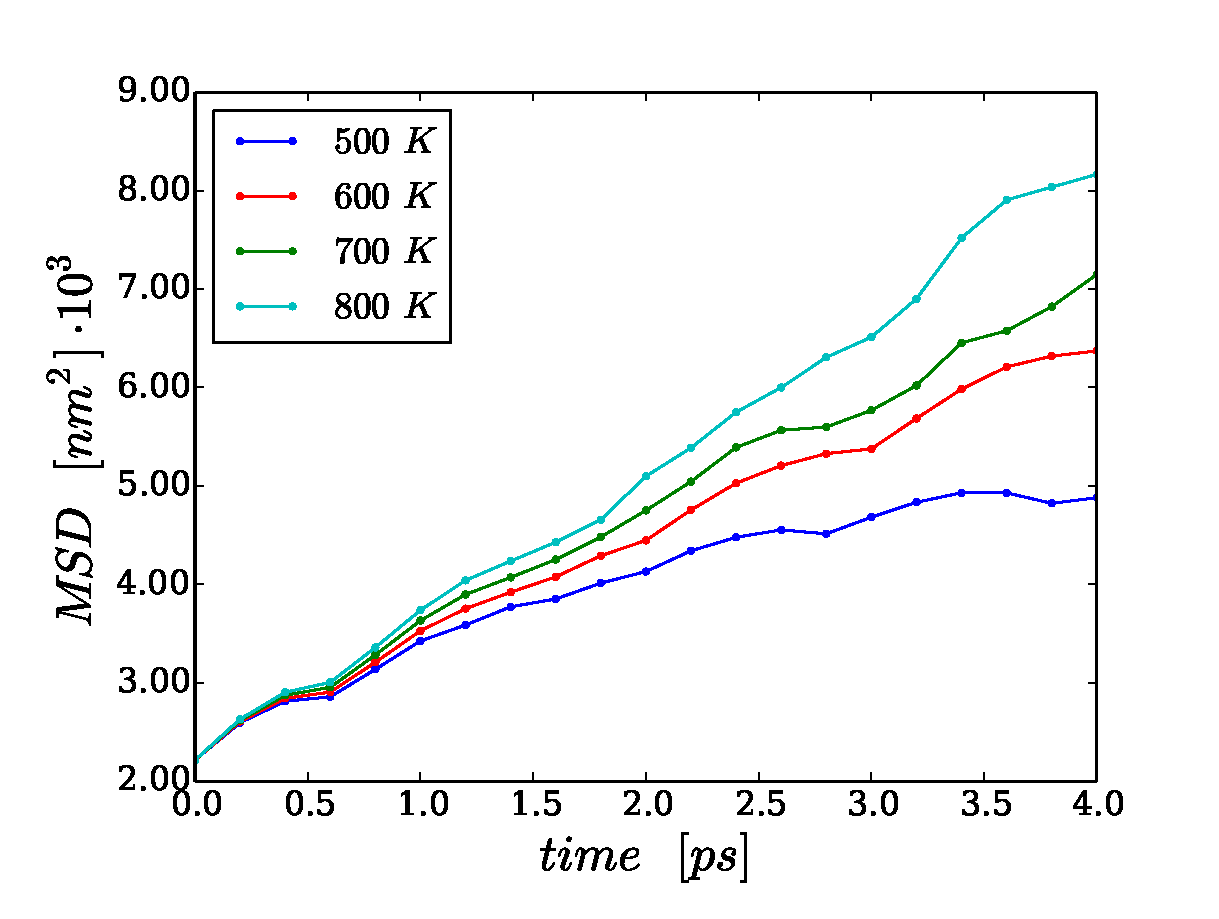
\includegraphics[width=10cm]{Cap_4/heatingFCC_500_800.pdf}
	\label{C4:fg:heating500_800_FCC}}
\\
\subfloat[Nanopartícula CuZr-B2]{
	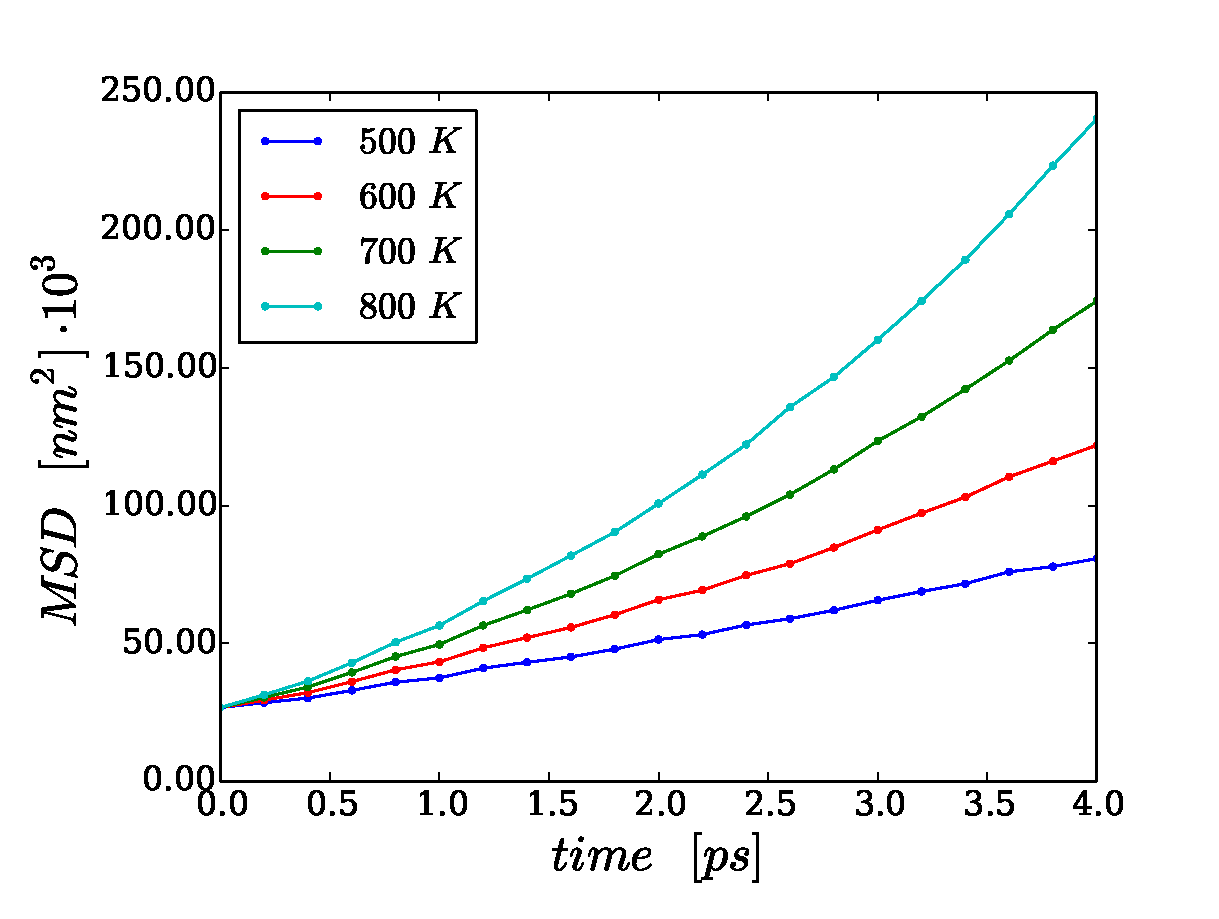
\includegraphics[width=10cm]{Cap_4/heatingB2_500_800.pdf}
	\label{C4:fg:heating500_800_B2}}
\caption[MSD para t $ \leq 4 $ ns. Ambas nanopartículas]{MSD para t $ \leq 4 $ ns. Ambas nanopartículas}
\label{C4:fg:heating_FCC_B2}
\end{figure}

\subsection{Carga Uniaxial del BMG}
\label{S4_3_2}

En esta sección, presentamos resultados sobre el sometimiento a esfuerzos uniaxiales del BMG que contiene una nanopartícula, como se describió anteriormente.

Las Figuras \ref{C4:fg:fcc_vm_tension} a \ref{C4:fg:b2_vm_compression} muestran el comportamiento esfuerzo-deformación de la muestra bajo esfuerzos uniaxiales de tracción y compresión a diferentes temperaturas. La apariencia de estas curvas sigue un comportamiento esperado observado para el material sin ninguna inclusión. La pequeña inclusión no afecta el régimen elástico, y a una temperatura elevada, el ablandamiento del BMG tampoco es afectado, tanto para tracción como para compresión. El esfuerzo máximo se ve decrementado ligeramente por la nanopartícula a bajas temperaturas. El esfuerzo de flujo plástico a grandes deformaciones no se ve modificado por la inclusión bajo compresión.

Si bien sería de esperar que los esfuerzos se concentren en la frontera entre la inclusión cristalina y la matriz amorfa, como vemos en las Figuras \ref{C4:fg:snapshot_ten_FCC_10K} a \ref{C4:fg:snapshot_comp_B2_400K} en general encontramos deformación plástica homogénea con nucleación abundante de STZs, probablemente debido a la alta velocidad de deformación y alta velocidad de templado de la muestra. Para el caso de esfuerzos de tracción (Figuras \ref{C4:fg:snapshot_ten_FCC_10K} a \ref{C4:fg:snapshot_ten_FCC_400K} y \ref{C4:fg:snapshot_ten_B2_10K} a \ref{C4:fg:snapshot_ten_B2_400K}) existe uno o más poros nucleados llegada una determinada deformación. El momento de su apertura coincide con la caída en el esfuerzo que observamos claramente en las Figuras \ref{C4:fg:fcc_vm_tension} y \ref{C4:fg:b2_vm_tension}. Para el caso de esfuerzos de compresión se observa un comportamiento similar en cuanto a la distribución homogénea de esfuerzos en la matriz amorfa.

La nucleación de los poros bajo tracción se ve algo retrasada por la inclusión, permitiendo alrededor de un 1\% de deformación adicional de la muestra en el caso general. Esto podría explicarse por alguna relajación y disipación ocurriendo en la frontera entre la nanopartícula y el BMG, pero un estudio más detallado debería realizarse para aclarar la situación ya que en el caso particular de la inclusión CuZr-B2 a 200 K observamos una caída anticipada del esfuerzo.

Como algunos poliedros de Voronoi son considerados ser estructuras más resistentes al esfuerzo cortante, particularmente las agrupaciones de icosaedros \citep{cheng08}, mostramos la evolución de la fracción de icosaedros en la muestra y la comparamos con la muestra de BMG original sin inclusiones y a 10 K. Podemos ver en la \fref{C4:fg:fcc_voro_10K} que las fracciones siguen el mismo comportamiento que en la muestra sin nanopartícula. Bajo tracción, la nucleación de un poro da origen a fluctuaciones. Vale la pena notar que estas fluctuaciones corresponden a una deformación más elevada como ya se había mencionado para la curva de esfuerzo-deformación.

\begin{figure}[htp]
\centering
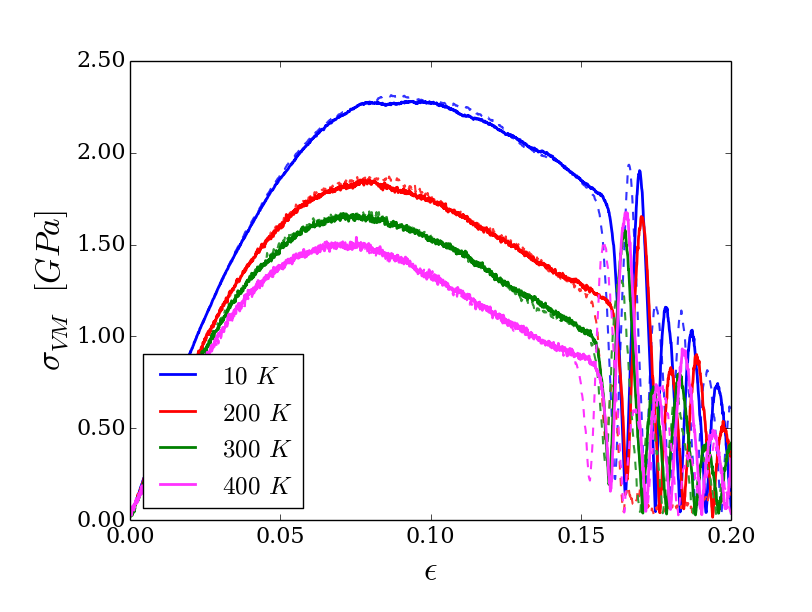
\includegraphics[width=10cm]{Cap_4/stress_strain_tension_FCC_NoInc.png}
\caption[Von Mises vs deformación en tracción. Inclusión Cu-FCC]{Tensión de Von Mises vs deformación para el BMG bajo esfuerzo uniaxial de tracción sin inclusión (línea punteada) y una inclusión de Cu-FCC (línea sólida)}
\label{C4:fg:fcc_vm_tension}
\end{figure}

\begin{figure}[htp]
\centering
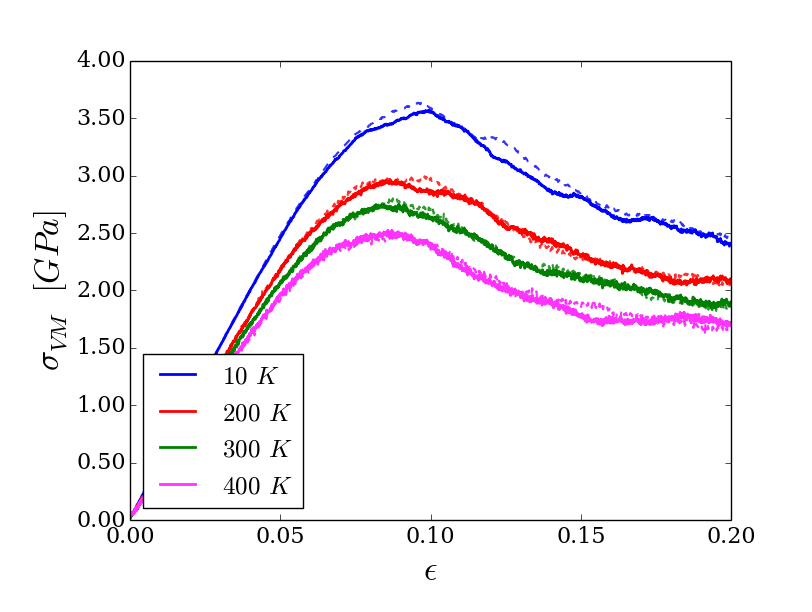
\includegraphics[width=10cm]{Cap_4/stress_strain_compression_FCC_NoInc.png}
\caption[Von Mises vs deformación en compresión. Inclusión de Cu-FCC]{Tensión de Von Mises vs deformación para el BMG bajo esfuerzo uniaxial de compresión sin inclusión (línea punteada) y una inclusión de Cu-FCC (línea sólida)}
\label{C4:fg:fcc_vm_compression}
\end{figure}

\begin{figure}[htp]
\centering
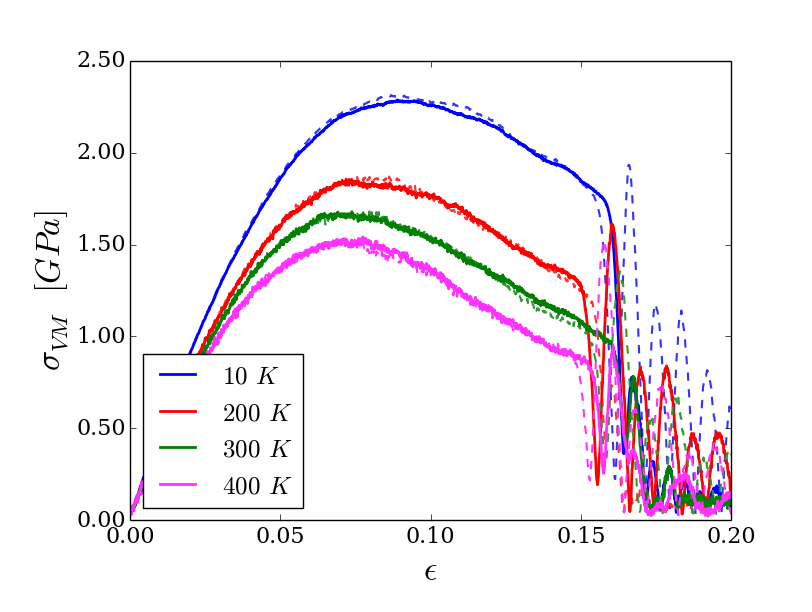
\includegraphics[width=10cm]{Cap_4/stress_strain_tension_B2_NoInc.png}
\caption[Von Mises vs deformación en tracción. Inclusión de CuZr-B2]{Tensión de Von Mises vs deformación para el BMG bajo esfuerzo uniaxial de tracción sin inclusión (línea punteada) y una inclusión de CuZr-B2 (línea sólida)}
\label{C4:fg:b2_vm_tension}
\end{figure}

\begin{figure}[htp]
\centering
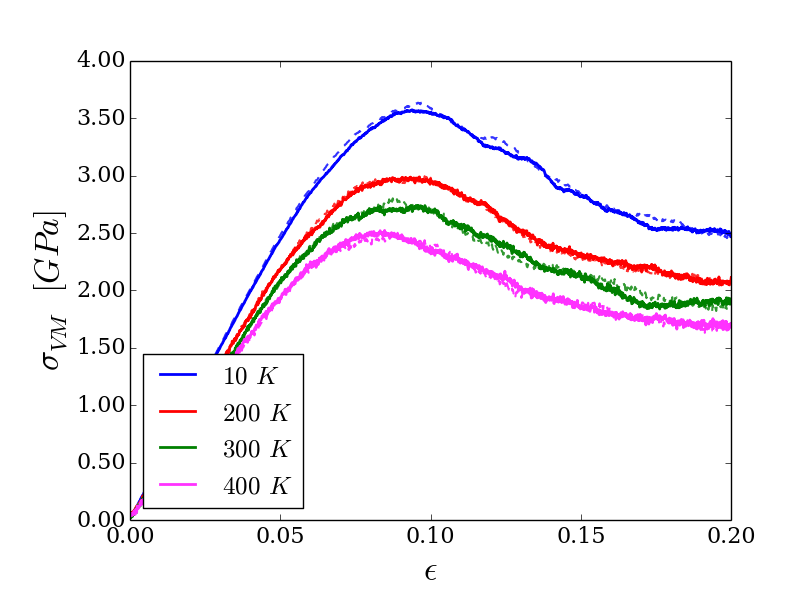
\includegraphics[width=10cm]{Cap_4/stress_strain_compression_B2_NoInc.png}
\caption[Von Mises vs deformación en compresión. Inclusión de CuZr-B2]{Tensión de Von Mises vs deformación para el BMG bajo esfuerzo uniaxial de compresión sin inclusión (línea punteada) y una inclusión de CuZr-B2 (línea sólida)}
\label{C4:fg:b2_vm_compression}
\end{figure}

\begin{figure}[htp]
\centering
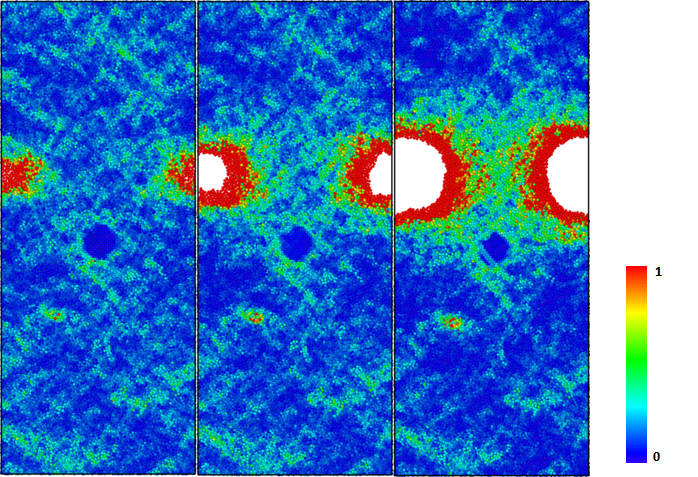
\includegraphics[width=10cm]{../ResumenImagenes/Figures/NanoParticles/Snapshots/cuSphereTension_10K_Snapshots.png}
\caption[Inclusión de Cu-FCC bajo tracción a 10K]{Inclusión de Cu-FCC bajo tracción a 10K}
\label{C4:fg:snapshot_ten_FCC_10K}
\end{figure}

% \begin{figure}[htp]
% \centering
% 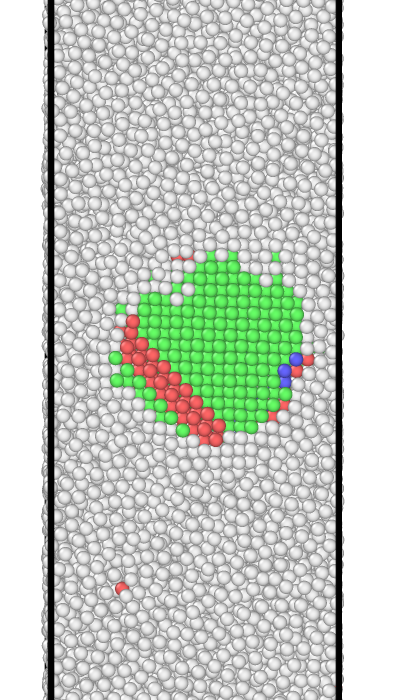
\includegraphics[width=10cm]{../ResumenImagenes/Figures/NanoParticles/cuSphereTension_10K_Snapshot_670_Macla_A.png}
% \caption{Dislocación al traccionar la muestra con nanopartícula de Cu-FCC a 10K (A). Verde: FCC, Rojo: HCP}
% \label{C4:fg:dislocacion_A}
% \end{figure}
% 
% \begin{figure}[htp]
% \centering
% 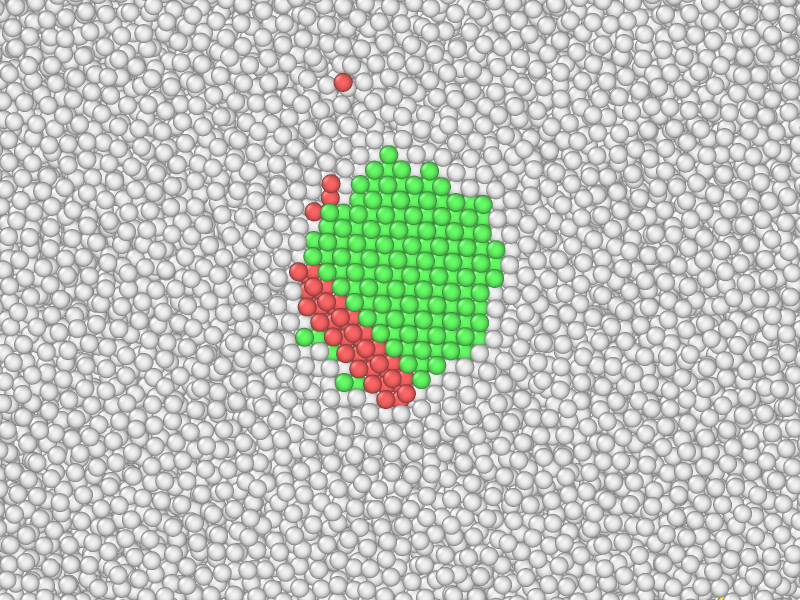
\includegraphics[width=10cm]{../ResumenImagenes/Figures/NanoParticles/cuSphereTension_10K_Snapshot_670_Macla_B.png}
% \caption{Dislocación al traccionar la muestra con nanopartícula de Cu-FCC a 10K (B). Verde: FCC, Rojo: HCP}
% \label{C4:fg:dislocacion_B}
% \end{figure}

\begin{figure}[htp]
\centering
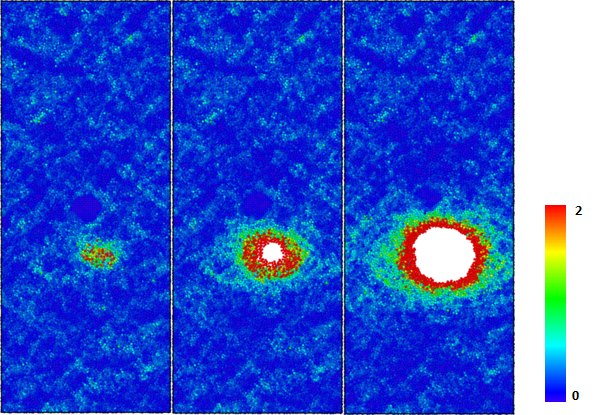
\includegraphics[width=10cm]{../ResumenImagenes/Figures/NanoParticles/Snapshots/cuSphereTension_200K_Snapshots.png}
\caption[Inclusión de Cu-FCC bajo tracción a 200K]{Inclusión de Cu-FCC bajo tracción a 200K}
\label{C4:fg:snapshot_ten_FCC_200K}
\end{figure}

\begin{figure}[htp]
\centering
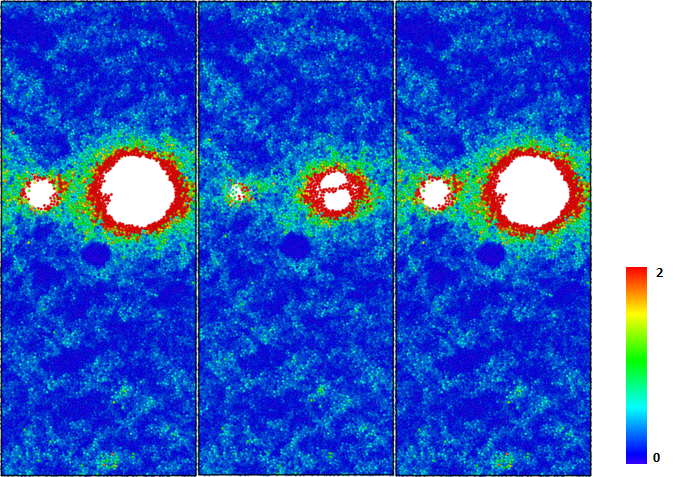
\includegraphics[width=10cm]{../ResumenImagenes/Figures/NanoParticles/Snapshots/cuSphereTension_400K_Snapshots.png}
\caption[Inclusión de Cu-FCC bajo tracción a 400K]{Inclusión de Cu-FCC bajo tracción a 400K}
\label{C4:fg:snapshot_ten_FCC_400K}
\end{figure}

\begin{figure}[htp]
\centering
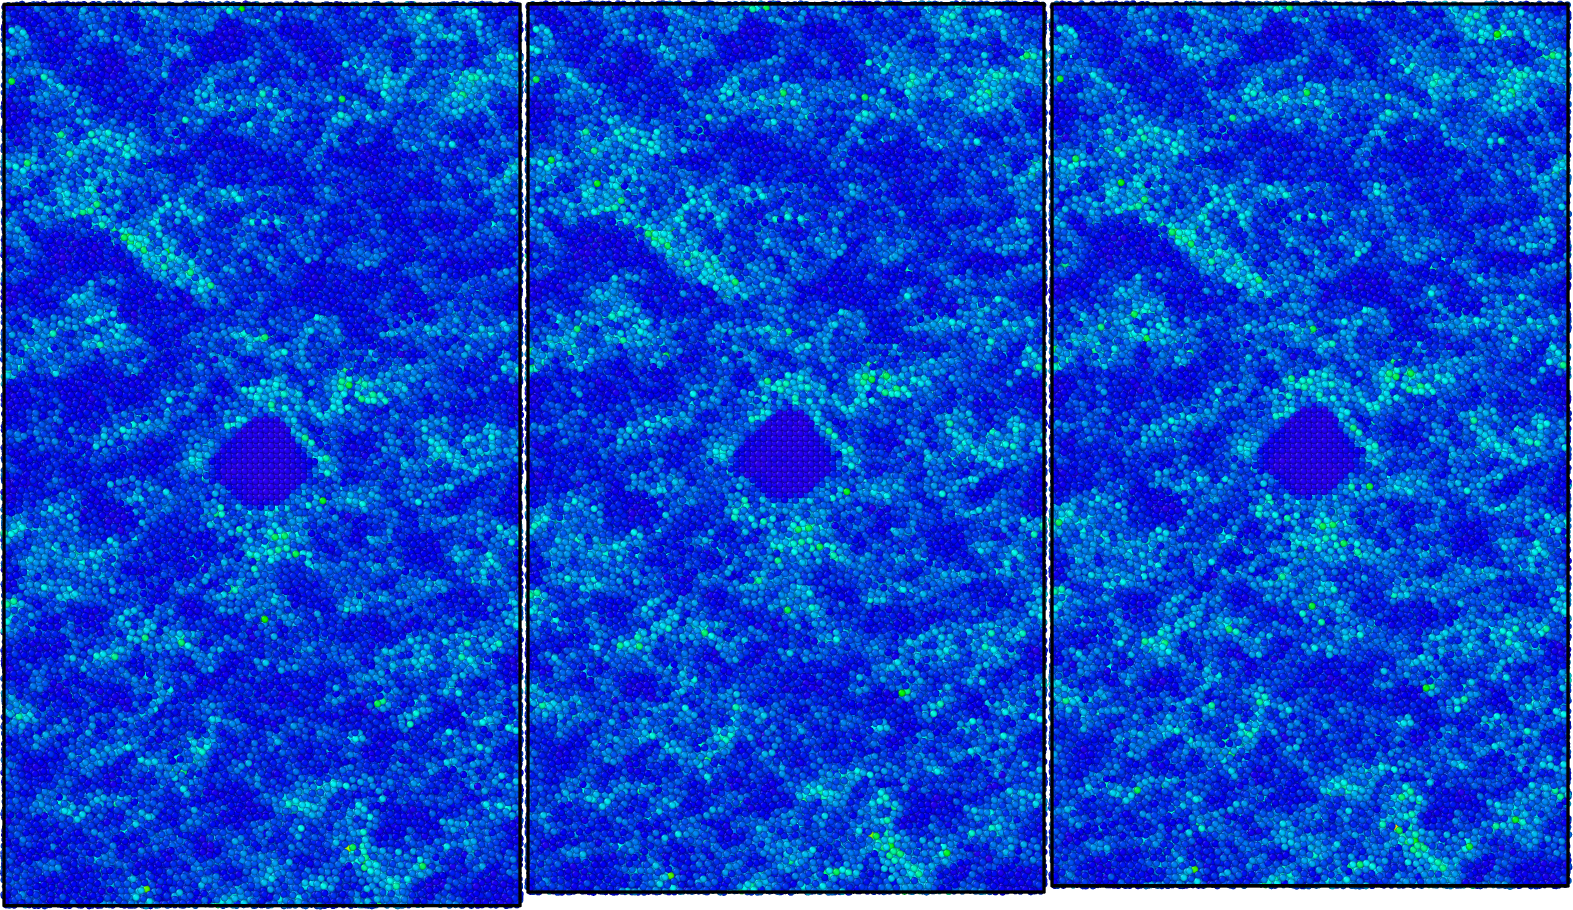
\includegraphics[width=10cm]{../ResumenImagenes/Figures/NanoParticles/Snapshots/cuSphereCompression_10K_Snapshots.png}
\caption[Inclusión de Cu-FCC bajo compresión a 10K]{Inclusión de Cu-FCC bajo compresión a 10K}
\label{C4:fg:snapshot_comp_FCC_10K}
\end{figure}

\begin{figure}[htp]
\centering
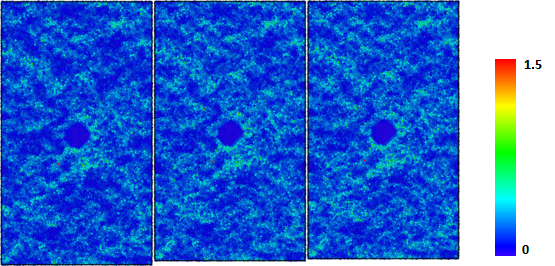
\includegraphics[width=10cm]{../ResumenImagenes/Figures/NanoParticles/Snapshots/cuSphereCompression_200K_Snapshots.png}
\caption[Inclusión de Cu-FCC bajo compresión a 200K]{Inclusión de Cu-FCC bajo compresión a 200K}
\label{C4:fg:snapshot_comp_FCC_200K}
\end{figure}

\begin{figure}[htp]
\centering
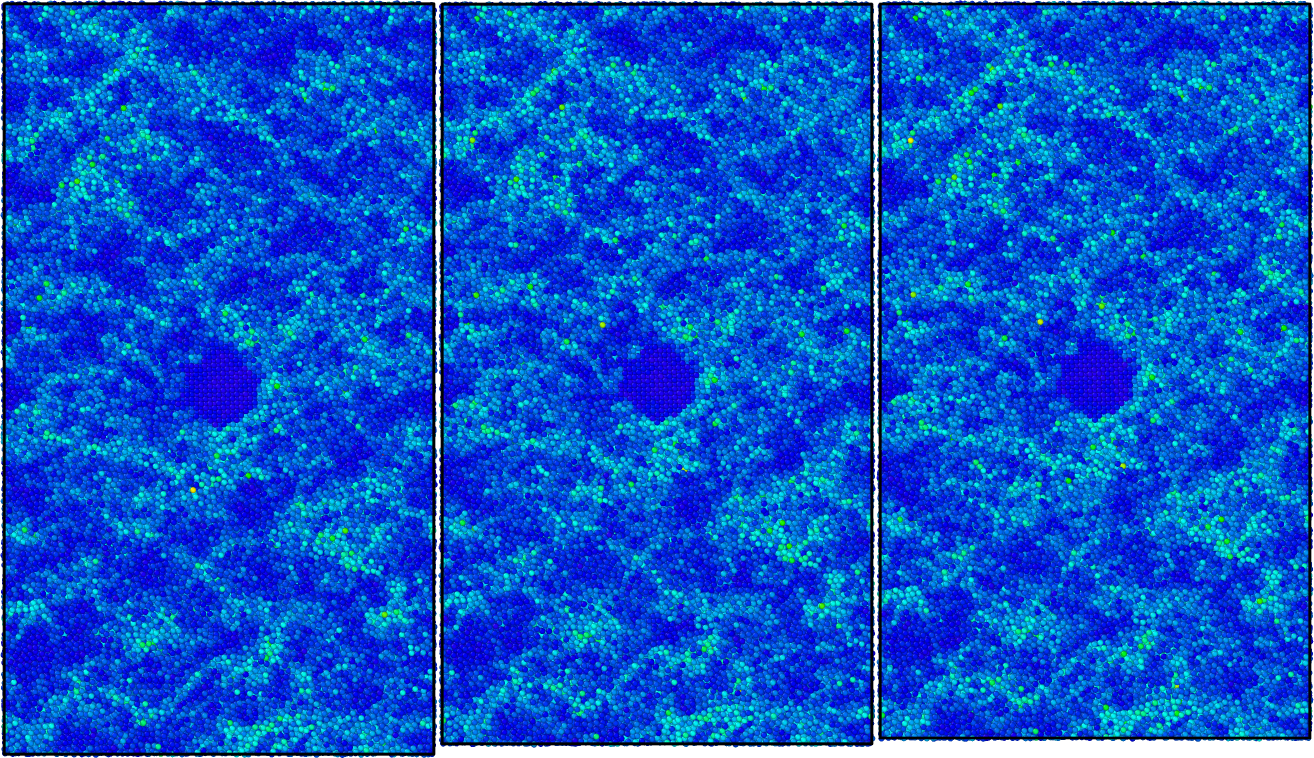
\includegraphics[width=10cm]{../ResumenImagenes/Figures/NanoParticles/Snapshots/cuSphereCompression_300K_Snapshots.png}
\caption[Inclusión de Cu-FCC bajo compresión a 300K]{Inclusión de Cu-FCC bajo compresión a 300K}
\label{C4:fg:snapshot_comp_FCC_300K}
\end{figure}

\begin{figure}[htp]
\centering
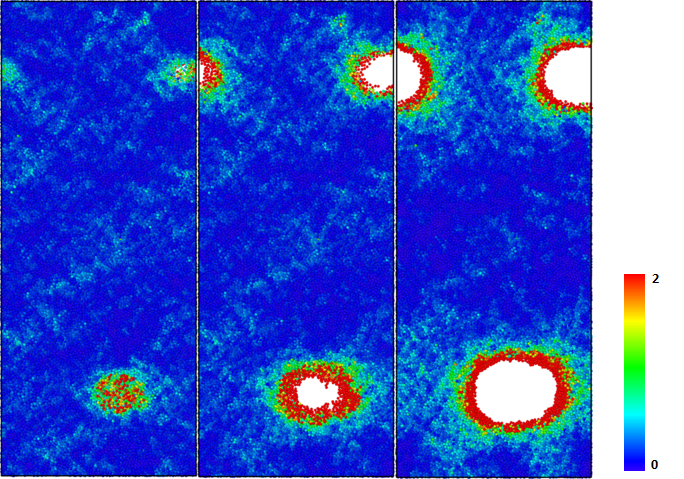
\includegraphics[width=10cm]{../ResumenImagenes/Figures/NanoParticles/Snapshots/B2SphereTension_10K_Snapshots.png}
\caption[Inclusión de CuZr-B2 bajo tracción a 10K]{Inclusión de CuZr-B2 bajo tracción a 10K}
\label{C4:fg:snapshot_ten_B2_10K}
\end{figure}

\begin{figure}[htp]
\centering
\includegraphics[width=10cm]{../ResumenImagenes/Figures/NanoParticles/Snapshots/B2SphereTension_200K_Snapshots.png}
\caption[Inclusión de CuZr-B2 bajo tracción a 200K]{Inclusión de CuZr-B2 bajo tracción a 200K}
\label{C4:fg:snapshot_ten_B2_200K}
\end{figure}

\begin{figure}[htp]
\centering
\includegraphics[width=10cm]{../ResumenImagenes/Figures/NanoParticles/Snapshots/B2SphereTension_300K_Snapshots.png}
\caption[Inclusión de CuZr-B2 bajo tracción a 300K]{Inclusión de CuZr-B2 bajo tracción a 300K}
\label{C4:fg:snapshot_ten_B2_300K}
\end{figure}

\clearpage

\begin{figure}[htp]
\centering
\includegraphics[width=10cm]{../ResumenImagenes/Figures/NanoParticles/Snapshots/B2SphereTension_400K_Snapshots.png}
\caption[Inclusión de CuZr-B2 bajo tracción a 400K]{Inclusión de CuZr-B2 bajo tracción a 400K}
\label{C4:fg:snapshot_ten_B2_400K}
\end{figure}

\begin{figure}[htp]
\centering
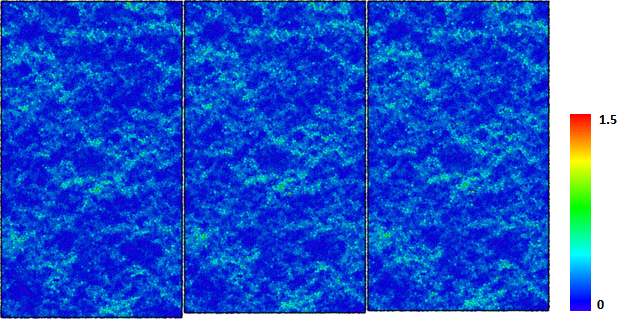
\includegraphics[width=10cm]{../ResumenImagenes/Figures/NanoParticles/Snapshots/B2SphereCompression_10K_Snapshots.png}
\caption[Inclusión de CuZr-B2 bajo compresión a 10K]{Inclusión de CuZr-B2 bajo compresión a 10K}
\label{C4:fg:snapshot_comp_B2_10K}
\end{figure}

\begin{figure}[htp]
\centering
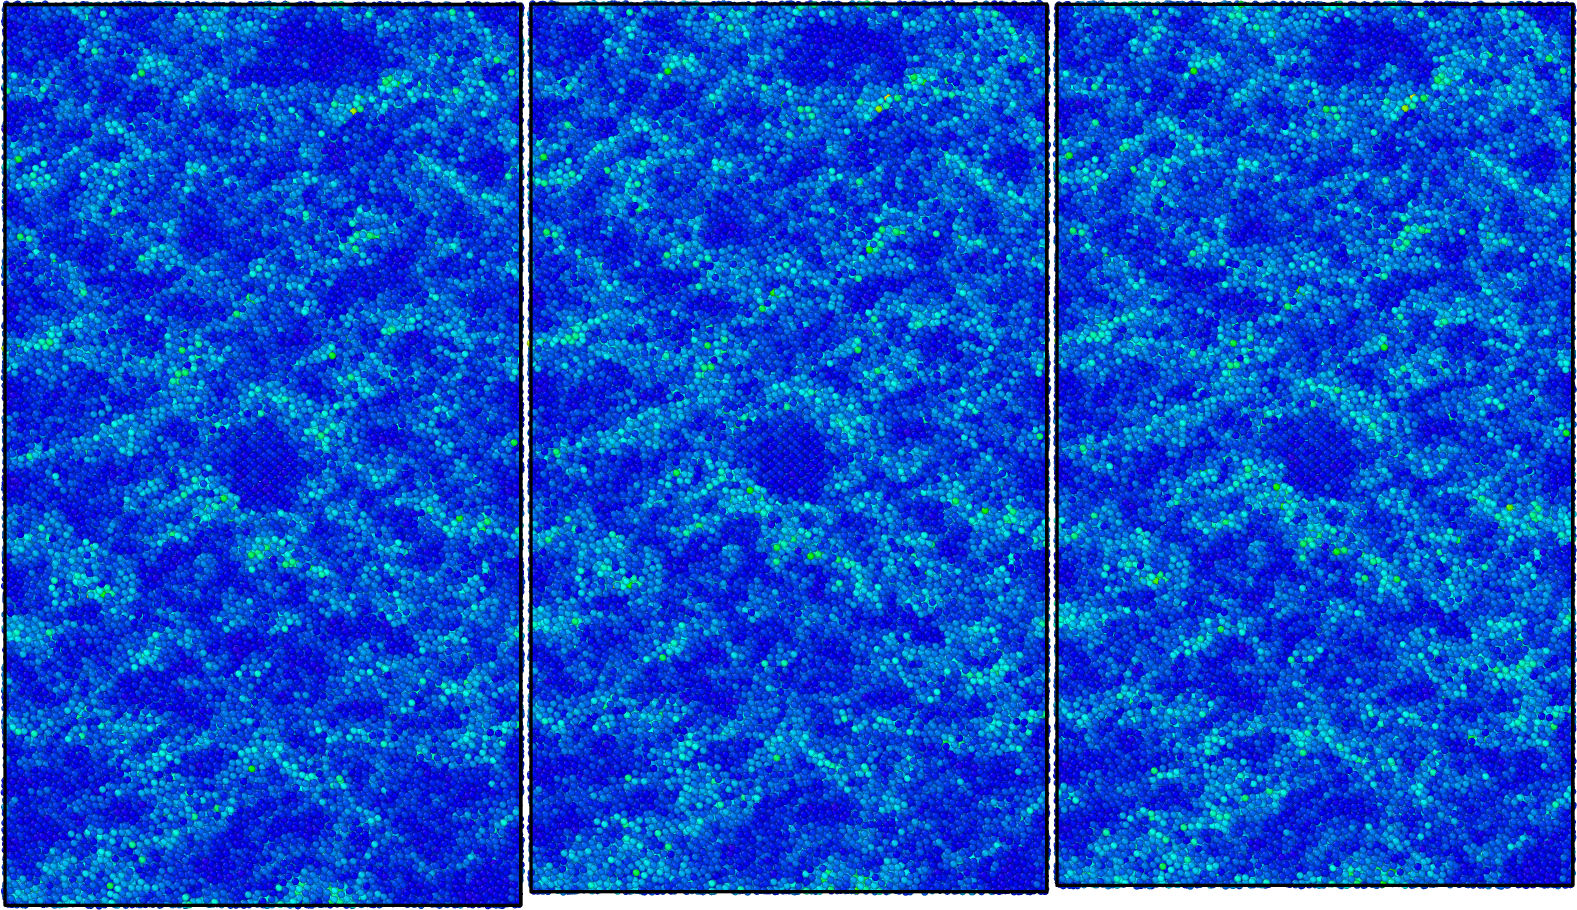
\includegraphics[width=10cm]{../ResumenImagenes/Figures/NanoParticles/Snapshots/B2SphereCompression_200K_Snapshots.png}
\caption[Inclusión de CuZr-B2 bajo compresión a 200K]{Inclusión de CuZr-B2 bajo compresión a 200K}
\label{C4:fg:snapshot_comp_B2_200K}
\end{figure}

\begin{figure}[htp]
\centering
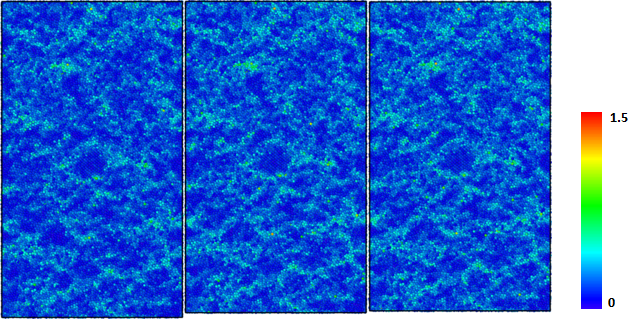
\includegraphics[width=10cm]{../ResumenImagenes/Figures/NanoParticles/Snapshots/B2SphereCompression_300K_Snapshots.png}
\caption[Inclusión de CuZr-B2 bajo compresión a 300K]{Inclusión de CuZr-B2 bajo compresión a 300K}
\label{C4:fg:snapshot_comp_B2_300K}
\end{figure}

\begin{figure}[htp]
\centering
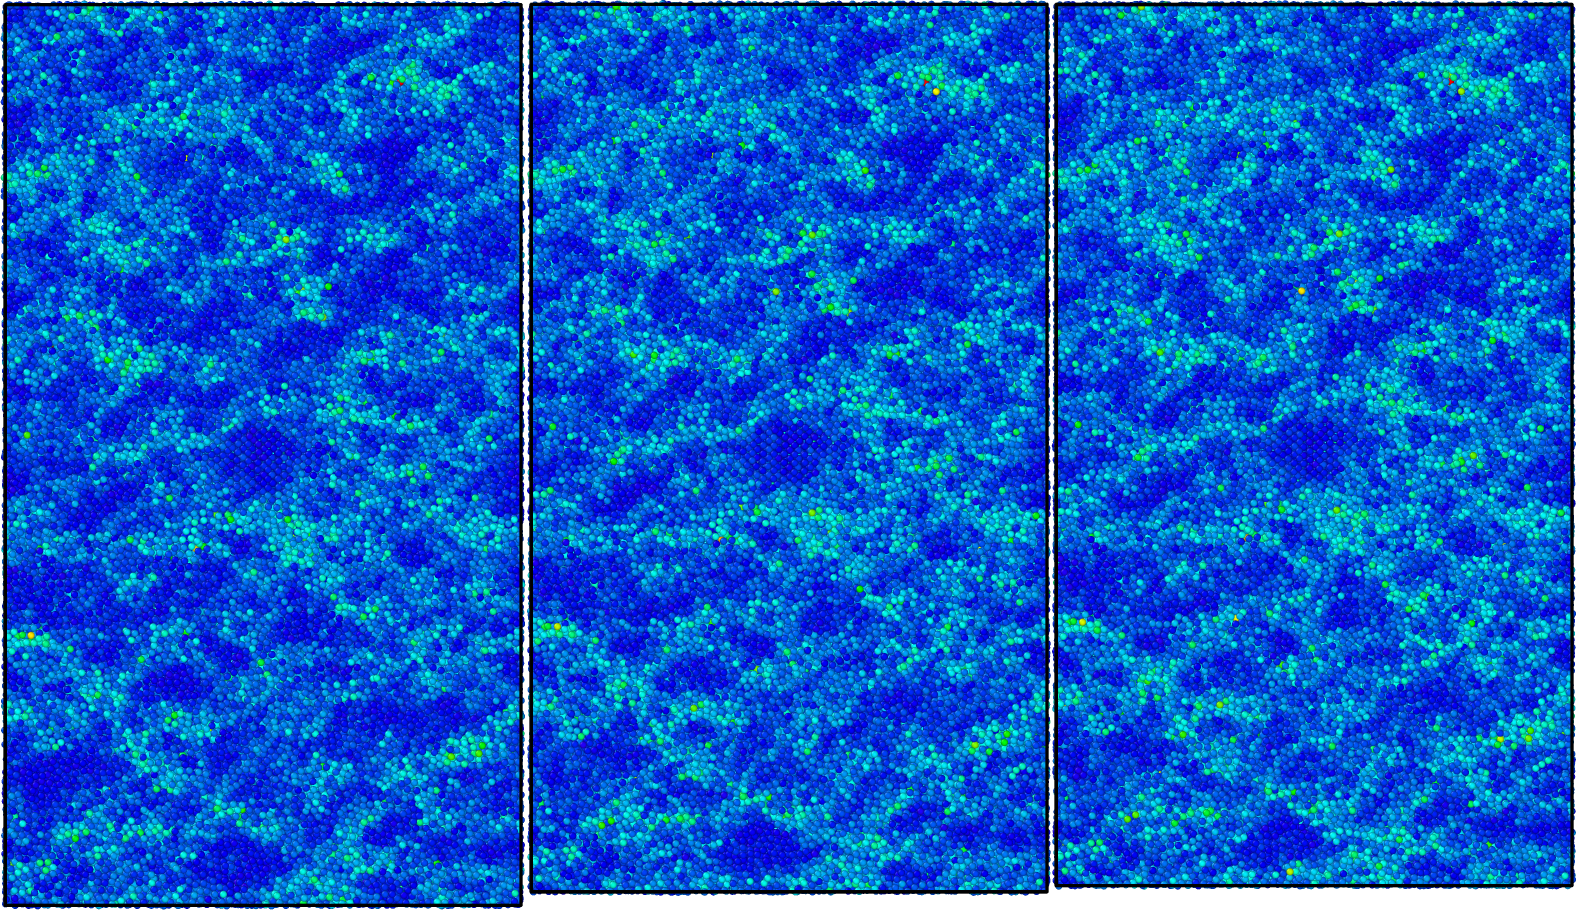
\includegraphics[width=10cm]{../ResumenImagenes/Figures/NanoParticles/Snapshots/B2SphereCompression_400K_Snapshots.png}
\caption[Inclusión de CuZr-B2 bajo compresión a 400K]{Inclusión de CuZr-B2 bajo compresión a 400K}
\label{C4:fg:snapshot_comp_B2_400K}
\end{figure}

\begin{figure}[htp]
\centering
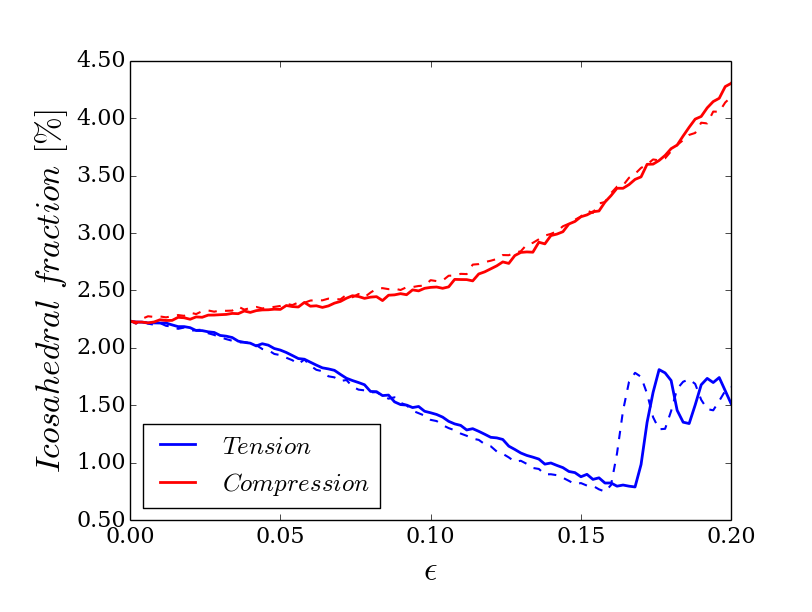
\includegraphics[width=12cm]{Cap_4/FCC_voro_vs_strain_10K_B.png}
\caption[Fracción de icosaedros a 10K]{Fracción de icosaedros bajo tracción y compresión a 10 K. La línea punteada representa la muestra original.}
\label{C4:fg:fcc_voro_10K}
\end{figure}

% \section{Resumen y Conclusiones}
% \label{S4_4}
% 
% Estudiamos un BMG con una nanopartícula cristalina como inclusión. Consideramos un vidrio CuZr, y una nanopartícula de Cu pura con un radio de 2 nm. Ésto implica una fracción en volumen que varía desde 1.15\% a 10 K hasta 1.12\% a 800 K como resultado del aumento del volumen inicial de la muestra con la temperatura. Una situación similar fue explorada recientemente por Albe et al. \citep{albe13}. Aquí, nos centramos en los efectos de la temperatura, e inicialmente estudiamos la estabilidad debajo de los 400 K, indicando que la nanopartícula es bastante estable a esas temperaturas. A temperaturas mayores, la difusividad en sólo algunos ns trae consigo la pérdida de una interfaz nítida entre la nanopartícula y la matriz.
% 
% En nuestras simulaciones, se aplicaron condiciones de frontera periódicas en tres dimensiones, y la ausencia de superficies libres deja sólo a la nanopartícula como probable concentrador de esfuerzo para promover la nucleación de STZs, y así desencadenar las bandas de corte, en la interfaz entre la matriz y la nanopartícula. Sin embargo, éste no fue el caso. Las curvas de esfuerzo-deformación son claramente similares al caso sin nanopartícula, a excepción de un retardo en la nucleación de un poro bajo tracción para la muestra con una nanopartícula.
% 
% El análisis de Voronoi no muestra diferencias significativas entre las muestras con y sin inclusión de nanopartícula. Un estudio futuro y más detallado es requerido para diferentes modos de carga y temperaturas. Estudios futuros también podrían repetir estos experimentos con inclusiones de CuZr con una estructura cristalina B2, como podemos encontrar en algunas experiencias \citep{wei14,kuo14}. 
% Chapter Template

\chapter{ESTUDIO DE LAS PROPIEDADES MECANICAS DE UN BMG POROSO SINTERIZADO (NANOVIDRIOS)} % Main chapter title

\label{C5} % Change X to a consecutive number; for referencing this chapter elsewhere, use \ref{ChapterX}

\lhead{Capítulo 5. \emph{ESTUDIO DE LAS PROPIEDADES MECANICAS DE UN BMG POROSO SINTERIZADO (NANOVIDRIOS)}} % Change X to a consecutive number; this is for the header on each page - perhaps a shortened title


%----------------------------------------------------------------------------------------
%	SECTION 1
%----------------------------------------------------------------------------------------

\section{Introducción}
\label{S5_1}

% Un vidrio metálico (MG), también llamado ``metal amorfo'', es una aleación metálica que posee una estructura amorfa,
% en oposición a la estructura cristalina que normalmente presentan los metales. Esto puede lograrse mediante varias técnicas,
% la mayoría de las cuales incluyen altas velocidades de temple, peque\~nos volúmenes y el control de la composición del
% material \citep{liebermann93}. Como resultado, estos materiales cuentan con algunas ventajas con respecto a los metales cristalinos:
% mejor elasticidad combinada con una alta resistencia, dureza y moldeabilidad \citep{telford04}.

% Existen dos enfoques principales para simular vidrios metálicos sometidos a deformación plástica: haciendo foco en el comportamiento
% a escala nanométrica \citep{ogata06,guan10} o utilizando mecánica del continuo \citep{malvern69}. Para el primer enfoque, las simulaciones
% con dinámica molecular (MD) son frecuentemente utilizadas \citep{allen87}. La dinámica molecular puede resolver problemas en los cuales
% interactuan muchos cuerpos (átomos), mediante la aplicación de un potencial entre pares de átomos. Así, este enfoque es útil para el
% estudio de propiedades a escala nanométrica, tal como la deformación, la tensión, la temperatura, etc.

% Las simulaciones con dinámica molecular también son útiles para identificar procesos pláticos en BMGs. La plasticidad comienza con la
% formación de zonas de transformación de tensión cortante (STZ), las cuales se nuclean, formando bandas de corte \citep{ogata06,shimizu07} a medida que la
% deformación aumenta. Las bandas de corte (SB) pueden provocar la falla frágil del material debido a la deformación heterogénea. De allí la importancia
% de prevenir o retrasar su propagación. En los metales cristalinos se procede de forma similar al trabar las dislocaciones.

Los vidrios metálicos con porosidad han sido objeto de mucho estudio en los últimos años \citep{guan13,wang10}, en un esfuerzo
por mejorar el entendimiento de su mecánica de deformación. El comportamiento en el
régimen elastoplástico puede ser controlado mediante la introducción de poros.

Las grandes deformaciones normalmente se deben, como se ha visto en capítulos anteriores, al colapso de zonas de transformación de
tensión cortante (STZ) que dan lugar a una o varias bandas de corte (SB), las cuales pueden provocar la falla frágil del material debido a la
deformación heterogénea. De allí la importancia de prevenir o retrasar su propagación.

La adición de poros en metales cristalinos reduce, como es sabido, el movimiento de dislocaciones y modifica la
deformación plástica resultante. De igual manera, los poros en vidrios metálicos limitan la propagación de bandas de corte y permiten
una deformación más homogénea. Ultimamente, se ha suscitado un gran interés al respecto, y varias opciones han sido exploradas
\citep{guan13,wang10,schuh07,liontas14}.

En el presente capítulo fabricamos muestras de BMG Cu$_{46}$ Zr$_{54}$ con porosidad
(similar a las muestras de ``nanovidrios'' en otros experimentos y simulaciones \citep{adibi13,albe13}) mediante el sinterizado de nanopartículas.
Las simulaciones con dinámica molecular nos permitirán analizar los polyedros de Voronoi, las tensiones y deformaciones atómicas,
así como también la forma en que la porosidad inicial afecta la deformación resultante de la muestra.

% En un trabajo previo hemos determinado los parámetros constitutivos del vidrio metálico Cu$_{46}$ Zr$_{54}$ como
% una función de la temperatura. Ahora presentamos resultados para un vidrio metálico de igual composición, pero
% fabricado mediante el sinterizado de nanopartículas de BMG, lo cual resulta en muestras con porosidad, similar
% a las muestras de ``nanovidrios'' en otros experimentos y simulaciones \citep{adibi13,albe13}. Para llevar a cabo las simulaciones atomísticas
% hemos utilizado el enfoque de Dinámica Molecular (MD), y el estudio incluye análisis de los polyedros de Voronoi, tensiones
% y deformaciones atómicas. Analizamos de qué forma depende la deformación en la fracción de volumen sólido (SVF), y cómo la deformación
% se distribuye a lo largo de la muestra en función de la porosidad inicial.

% Una deformación más homogénea puede ser lograda mediante el agregado de nanoinclusiones al material. Ultimamente, se ha suscitado
% un gran interés al respecto, y varias opciones han sido exploradas \citep{guan13,wang10,schuh07,liontas14}. Siguiendo trabajo previo, en el
% presente trabajo fabricamos muestras de BMG Cu$_{46}$ Zr$_{54}$ con porosidad (similar a las muestras de ``nanovidrios'' en otros
% experimentos y simulaciones \citep{adibi13,albe13}) mediante el sinterizado de nanopartículas. Las simulaciones con dinámica molecular
% nos permitirán analizar los polyedros de Voronoi, las tensiones y deformaciones atómicas, así como también la forma en que la porosidad inicial
% afecta la deformación resultante de la muestra.

%----------------------------------------------------------------------------------------
%	SECTION 2
%----------------------------------------------------------------------------------------

\section{Detalles de Simulación y Preparación de la Muestra Porosa}
\label{S5_2}

% Para este trabajo, las simulaciones con dinámica molecular fueron realizadas mediante el uso del programa LAMMPS \citep{plimpton95},
% el cual es gratuito y de código libre, tiene un muy buen manual y es computacionalmente eficiente para la simulación de sistemas
% con gran número de átomos. Por otro lado, el análisis de Voronoi y las imágenes de la muestra fueron realizadas con el programa Ovito
% \citep{stukowski10}, y otras figuras fueron graficadas con Gnuplot. Ambos programas son gratuitos y de código libre.

\begin{figure}[h!]
  \centering
  \begin{tabular} {c}
    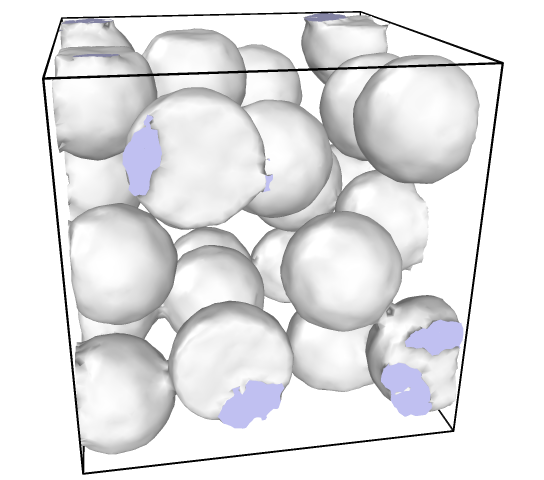
\includegraphics[width=10cm]{Cap_5/spheres2.png}\\
    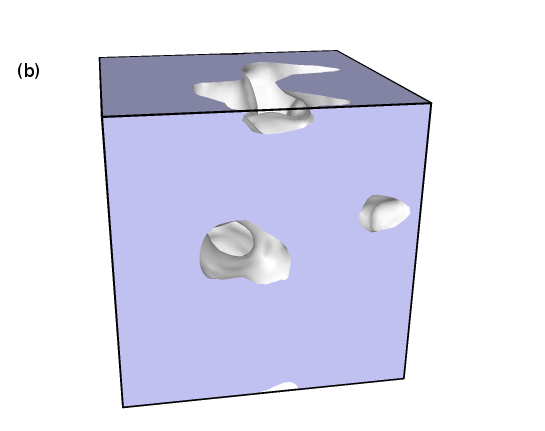
\includegraphics[width=10cm]{Cap_5/spheres3.png}\\
  \end{tabular}
  \caption[Imágenes de la muestra]{Imágenes de la muestra (a) anterior al proceso de sinterizado y (b) posterior
  al proceso de sinterizado (porosidad 13\%).}
  \label{C5:fg:sint}
\end{figure}

Para la preparación de la muestra porosa, hemos tomado como punto de partida la misma muestra utilizada con anterioridad (capítulo \ref{C3}).
% y descripta por \cite{arman10}. Se trata de una muestra prismática Cu$_{46}$ Zr$_{54}$ con un total de 160000 átomos y obtenida
% mediante una velocidad de enfriamiento de 10$^{12}$ K/s. La temperatura de transición vítrea experimental (T$_{g}$) de este vidrio metálico
% es de 696 K, y el módulo de cizalladura (o módulo de elasticidad transversal G) es 30 GPa \citep{johnson05}. 
Para describir las interacciones
entre los átomos, usamos nuevamente el potencial EAM (método de átomo embebido) \citep{daw84}. Usamos condiciones de frontera periódicas en las
tres caras, lo cual es apropiado para altas velocidades de deformación \citep{bringa05}. De esta forma, podemos simular un BMG (de mayor tamaño)
y evitar concentración de tensiones en las fronteras.

Tomamos la muestra original y la replicamos a modo de obtener una muestra aproximadamente cúbica, de 15 nm de lado. Luego, seleccionamos puntos
al azar dentro de la muestra para hacer de centro de las esferas (de 2.5 nm de radio), y removimos todo el material al exterior de dichas esferas
para simular el sinterizado de nanopartículas esféricas de material. La figura~\ref{C5:fg:sint}-(a) muestra el resultado de estas acciones. Esta
nueva muestra tiene 77888 átomos.

El procedimiento para simular el sinterizado fue de relajar la muestra a una temperatura constante de 650K, justo debajo de la temperatura
de transición vítrea, y volúmen constante durante unos pocos ps, y luego aplicar hasta 10 ps de presión compresiva (400 bar). Estos dos pasos
fueron repetidos hasta lograr las porosidades deseadas. Luego, relajamos la muestra una vez más mediante el siguiente procedimiento: temple a 
temperatura cero mediante una velocidad de enfriamiento de $6.5 \cdot 10^{14} K/s$, aplicación de un baróstato para llegar a presión
cero, calentamiento a la misma velocidad que la velocidad de enfriamiento para llegar a la temperatura de simulacion (300K) y,
finalmente, aplicación de un baróstato durante 5 ps para reducir la presión a cero mientras se mantiene la temperatura constante. La 
figura~\ref{C5:fg:sint}-(b) exhibe una de las muestras obtenidas mediante el proceso que se ha explicado.

Se prepararon muestras con distintas porosidades iniciales (3.3\%, 5.8\% y 13.1\%). Estas muestras estabilizadas fueron luego utilizadas
para realizar carga uniaxial de compresión y tracción. Todas las coordenadas atómicas fueron recalculadas cada paso, en relación con la
velocidad de deformación requerida, la cual fue de $10^9 /s$, valor apropiado para experimentos de choque compresivo.

%----------------------------------------------------------------------------------------
%	SECTION 3
%----------------------------------------------------------------------------------------

\section{Resultados}
\label{S5_3}

A continuación presentamos resultados para deformación puramente uniaxial, la cual es adecuada para realizar comparaciones con resultados de
experimentos a altas velocidades de deformación, donde las deformaciones laterales pueden ser despreciadas.

\begin{figure}[h!]
  \centering
  \begin{tabular} {c}
    \includegraphics[width=10cm]{Cap_5/SVF_strain_comp_dash.eps}\\
    \includegraphics[width=10cm]{Cap_5/SVF_strain_tens.eps}\\
  \end{tabular}
  \caption[Fracción de volumen sólido (SVF) versus deformación.]{Fracción de volumen sólido (SVF) versus deformación. (a) Compresión
  (b) Tracción. En (a), las líneas a trazos indican la deformaión a la cual los poros se cierran por completo}
  \label{C5:fg:svf}
\end{figure}

La figura~\ref{C5:fg:svf} muestra la evolución de la densidad en las muestras porosas. Para el caso de compresión, hemos agregado unas líneas a trazos
que indican el punto en el que los poros se cierran completamente, es decir, la fracción de volumen sólido es igual a 1.
Para cada porosidad, el valor de deformación $\epsilon$ correspondiente es: 3\% $\rightarrow$ 0.05, 6\% $\rightarrow$ 0.065, 13\% $\rightarrow$ 0.12.
En algunas de las figuras de esta sección aparecerán estas líneas nuevamente, a fin de observar si este evento implica cambios en el comportamiento
plástico. Para el caso de tracción, el uso de condiciones de borde periódicas evita que los poros se cierren incluso a altas
deformaciones uniaxiales, dado que no hay deformaciones laterales.

\begin{figure}[h!]
  \centering
  \begin{tabular} {c}
    \includegraphics[width=10cm]{Cap_5/Pzz_strain_comp_dash.eps}\\
    \includegraphics[width=10cm]{Cap_5/Pzz_strain_tens.eps}\\
  \end{tabular}
  \caption[Presión en el eje Z vs deformación.]{Presión en el eje Z vs deformación. (a) Compresión (b) Tracción.}
  \label{C5:fg:pzz2}
\end{figure}

\begin{figure}[h!]
  \centering
  \begin{tabular} {c}
    \includegraphics[width=10cm]{Cap_5/stress_strain_comp_dash.eps}\\
    \includegraphics[width=10cm]{Cap_5/stress_strain_tens.eps}\\
  \end{tabular}
  \caption[Tensión de von Mieses vs deformación.]{Tensión de von Mieses vs deformación. (a) Compresión (b) Tracción.}
  \label{C5:fg:stress}
\end{figure}

La figura~\ref{C5:fg:pzz2}-(a) grafica la presión en el eje de carga versus deformación para esfuerzos de compresión. La figura~\ref{C5:fg:stress}-(a),
a su vez, grafica el esfuerzo de von Mieses versus deformación para esfuerzos de compresión.
Ambas gráficas nos indican que la presencia de porosidad promueve el inicio de la plasticidad. Los poros actúan como concentradores de tensión,
facilitando la aparición de STZs y bandas de corte. Esta plasticidad temprana comienza a
cerrar los poros, produciendo una curva donde la deformación $\epsilon$ aumenta mientras que la presión se mantiene baja.
Cuando los poros se cierran, la presión aumenta más aceleradamente, como puede apreciarse en la porción de la curva posterior
a la línea de trazos. Podemos también observar que el comportamiento de las muestras porosas luego de las líneas de trazos es
muy similar al comportamiento de la muestra sin porosidad, validando el hecho de que a ese punto ya no hay más porosidad. Basándonos en la figura,
podemos concluir que a mayor porosidad, se necesita menor esfuerzo para cerrar los poros (denotado por la altura de las líneas a trazos),
pero esto ocurre a mayores deformaciones.

En tracción las muestras se comportan diferentemente. Como ya se ha dicho los poros no se cierran en tracción, como sí lo hacían en compresión.
Mediante el análisis de algunas imágenes de la muestra, como las que aparecen en la figura~\ref{C5:fg:ss_tens},
observamos que los poros crecen a una velocidad aproximadamente constante a medida que la deformación de la muestra aumenta. 
Las figuras~\ref{C5:fg:pzz2}-(b) y \ref{C5:fg:stress}-(b) también muestran lo que parece ser flujo plástico: particularmente a 13\% porosidad,
pero similarmente a otras porosidades, luego de un cierto punto, la deformación aumenta mientras la presión se mantiene constante o
incluso disminuye.

\begin{figure}[h!]
  \centering
  \begin{tabular} {c}
    \includegraphics[width=10cm]{Cap_5/tipe3_strain_comp.eps}\\
    \includegraphics[width=10cm]{Cap_5/tipe3_strain_tens.eps}\\
  \end{tabular}
  \caption[Polyedros de Voronoi tipo 3 vs deformación.]{Polyedros de Voronoi tipo 3 vs deformación. (a) Compresión (b) Tracción.}
  \label{C5:fg:tip3}
\end{figure}

\begin{figure}[h!]
  \centering
  \begin{tabular}{c}
    \includegraphics[width=8cm]{Cap_5/13_0strain.png} \\
    \includegraphics[width=8cm]{Cap_5/13_5strain_comp.png}\includegraphics[width=8cm]{Cap_5/13_12strain_comp.png} \\
  \end{tabular}
  \caption[Coloreado de una sección de la muestra con porosidad 13\% según la deformación cortante.]{Coloreado de una sección de la muestra con
  porosidad 13\% según la deformación cortante. El coloreado fue hecho usando Ovito, el color azul siendo 0.1 o menor y el color rojo 0.3 o mayor.
  (a) Estado inicial de la muestra (b) 5\% deformación por compresión (c) 12\% deformación por compresión.}
  \label{C5:fg:ss_comp}
\end{figure}

\begin{figure}[h!]
  \centering
  \begin{tabular}{c}
    \includegraphics[width=8cm]{Cap_5/13_6strain_tens.png}\includegraphics[width=8cm]{Cap_5/13_20strain_tens.png} \\
  \end{tabular}
  \caption[Coloreado de una sección de la muestra con porosidad 13\% según la deformación cortante.]{Coloreado de una sección de la muestra con
  porosidad 13\% según la deformación cortante. El coloreado fue hecho usando Ovito, el color azul siendo 0.1 o menor y el color rojo 0.3 o
  mayor. (a) 6\% deformación por tracción (b) 20\% deformación por tracción.}
  \label{C5:fg:ss_tens}
\end{figure}

La figura~\ref{C5:fg:tip3} muestra curvas de polyedros de Voronoi versus deformación. El análisis por teselado de Voronoi es una técnica para
caracterizar el ordenamiento local en vidrios metálicos amorfos, donde cada átomo es el centro de un polyedro de Voronoi,
completado por sus vecinos más cercanos. En \cite{arman10}, los átomos de tipo 3 son identificados como indicadores de plasticidad, por eso
son de gran importancia.

La figura~\ref{C5:fg:tip3}-(a) presenta las curvas de polyedros de Voronoi para esfuerzos de compresión. El gráfico muestra una caída en el número
de los átomos tipo 3, la cual sucede luego de una fase constante. Se ha pensado en este fenómeno como un indicador del inicio de la plasticidad
\citep{arman10}. Sin embargo, nuestras curvas muestran un resultado contraintuitivo, ya que la plasticidad comienza antes en las muestras con menor
porosidad de acuerdo a nuestro análisis. Esto podría ser considerado como un indicador de que hay otros factores o procesos en juego que afectan
los resultados.

Las figuras~\ref{C5:fg:ss_comp}-(b) y (c) presentan la evolución de la deformación cortante en la muestra, para esfuerzos de compresión.
Salta inmediatamente a la vista que los poros actúan como concentradores de tensiones, pero también representan un obstáculo para la
propagación de bandas de corte \citep{wang10}. Las bandas de corte nuclean diagonalmente en el espacio entre poros, y la deformación atómica
se acumula a lo largo de estas direcciones principales por el resto de la simulación, como puede observarse en la imágen de la muestra a 
deformación 12\%. Un endurecimiento de la muestra ocurre algunos momentos previo al cierre total de los poros, tal y como a apreciado
\cite{yuan14} y puede verse en la figura~\ref{C5:fg:pzz2}-(a).

La figura~\ref{C5:fg:tip3}-(b) muestra las curvas de poledros de Voronoi para esfuerzos de tracción. En esta imágen, los átomos de tipo 3
prácticamente no varían en las muestras con porosidad, lo que implicaría que no hay formación de STZs.
Para la muestra no porosa, el número de átomos tipo 3 se vuelve aproximadamente constante luego de que se ha nucleado el poro. Esto
nos llevó a pensar que, dada las condiciones de las muestras, se facilita el movimiento de los átomos alrededor de los poros, lo cual evita
la formación de STZs fuera de los alrededores de los poros. Para apoyar esta idea, en las figuras~\ref{C5:fg:ss_tens}-(b) y (c) presentamos
la muestra coloreada con la deformación cortante. Es evidente que la deformación cortante se concentra principalmente alrededor
de los poros. Debe ser mencionado que la posición relativa entre átomos que se encuentran lejanos de los poros se mantiene aproximadamente igual.


%----------------------------------------------------------------------------------------
%	SECTION 4
%----------------------------------------------------------------------------------------

\section{Conclusiones}
\label{S5_4}

Se realizaron simulaciones de Dinámica Molecular (MD) en una muestra porosa del vidrio metálico Cu$_{46}$ Zr$_{54}$, aplicando esfuerzos
de compresión y tracción. Los resultados bajo deformación fueron comparables a aquellos encontrados en la literatura \citep{yuan14} para
la compresión de muestras porosas de monocristales de cobre. Esto puede ser considerado como una validación del proceso de sinterizado 
utilizado para la preparación de las muestras.

Con carga compresiva, los poros facilitan la plasticidad actuando como concentradores de tensiones, pero también retrasan
la formación de zonas de transformación de tensión cortante (STZs) y su posible unión en una banda de corte (SB), para el material lejano a los poros.
Los resultados también exhiben un endurecimiento de la muestra al cerrarse los poros, similarmente a lo que ocurre en el caso no poroso.

Con carga de tracción y deformación puramente uniaxial, los poros no cierran y concentran flujo plástico alrededor de ellos, a su vez
que también impiden la formación de STZs y bandas de corte.

% Estudios futuros incluirán un análisis de Voronoi profundizado y la simulación de muestras más grandes con topologías de porosidad diferentes.

 
% Chapter Template

\chapter{CONCLUSIONES} % Main chapter title

\label{C6} % Change X to a consecutive number; for referencing this chapter elsewhere, use \ref{ChapterX}

\lhead{Capítulo 6. \emph{CONCLUSIONES}} % Change X to a consecutive number; this is for the header on each page - perhaps a shortened title

%----------------------------------------------------------------------------------------
%	SECTION 1
%----------------------------------------------------------------------------------------

\section{Generales}

Se realizaron simulaciones atomísticas del comportamiento mecánico de vidrios metálicos volumétricos (BMGs) bajo diferentes modos de carga y con diferentes modificaciones a su composición haciendo uso de simulaciones de dinámica molecular (MD). En el \cref{C3} se estudia una matriz amorfa de cobre-circonio ($Cu_{46}Zr_{54}$) bajo tensiones de tracción y compresión y se observan los efectos de la temperatura en los parámetros constitutivos así como en la respuesta mecánica. Luego, en el \cref{C4}, se estudia la estabilidad de nanopartículas cristalinas en la matriz amorfa previamente caracterizada y se comprara el comportamiento mecánico con el aquél del \cref{C3}. Por último, en el \cref{C5}, nos enfocamos en analizar el impacto sobre el comportamiento mecánico de una matriz porosa al graduar la porosidad a diferentes niveles.

Como podemos observar en las curvas de tensión-deformación del \cref{C3}, el comportamiento tanto en tracción como en compresión de la muestra original presenta una variación suave en función de la temperatura, lo que vemos reflejado en los buenos ajustes obtenidos con un decremento exponencial con la temperatura (Figuras \ref{C3:fg:youngVsT}, \ref{C3:fg:peakVMisesVsT}, \ref{C3:fg:peakVMises1218VsT} y \ref{C3:fg:fitDosTercios}), típico de procesos activados térmicamente. Se observa un claro apartamiento del caso a 900 K del resto de las simulaciones, donde el incremento de la temperatura produce un decremento considerable del módulo elástico y de la tensión de Von Mises. Esto es de esperar al ser una temperatura muy superior a la temperatura de transición vítrea (696 K). Cabe destacar que en todos los casos se encuentra una asimetría en tracción y compresión, y los valores se encuentran más próximos sólo en el caso del módulo de Young (\fref{C3:fg:youngVsT}). Las tensiones máximas son mucho mayores en compresión.

Si bien un indicio de banda de corte (SB) puede observarse en la \fref{C3:fg:SBs}, no se observaron SBs claramente definidas como las que vemos en la \fref{C1:fg:shearbands}, lo que es de esperarse dado que nuestra muestra fue generada con una velocidad de enfriamiento muy elevada. Al no contar con la presencia de SBs, la identificación del comienzo de la plasticidad es muy compleja. Si bien podemos observar zonas de transformación del esfuerzo de corte (STZs), para un correcto análisis de las mismas sería necesario realizar simulaciones de una duración mucho mayor a las actuales. ESTE PARRAFO NO SE CORRESPONDE EXACTAMENTE CON LO QUE PONEMOS EN EL CAP 3 ( ??? ) Y, EN CIERTO MODO, DECIR QUE NO PODEMOS IDENTIFICAR EL COMIENZO DE LA PLASTICIDAD HARIA QUE LOS CAP. SIGUIENTES SE TRATEN DE BASICAMENTE NADA

Al estudiar los efectos de la temperatura sobre nanopartículas embebidas, los ajustes de difusividad en función de la temperatura pudieron realizarse para el caso de partícula Cu-FCC con $T \geq 500 K$ donde existen desplazamientos atómicos lo suficientemente importantes (\fref{C4:fg:msd500_800_FCC}). Esto puede interpretarse como el hecho de que la partícula es estable a temperaturas menores a 500 K, es decir, no se disuelve en la matriz. Sin embargo, a temperaturas más elevadas los átomos difunden y se pierde la estructura cristalina y con esto la interfase definida entre material cristalino y amorfo. Observando las curvas de desplazamientos para el caso de la partícula CuZr-B2 (Figuras \ref{C4:fg:msd10_400_B2} y \ref{C4:fg:msd500_800_B2}) vemos una pendiente cercana a cero en todos los casos, lo que dificulta el ajuste de difusividad. Si bien esto puede interpretarse como la estabilidad de la partícula, hay que tener en cuenta que los desplazamientos iniciales en iguales condiciones son mucho mayores para la partícula CuZr-B2 que para Cu-FCC (Figuras \ref{C4:fg:msd500_800_FCC} y \ref{C4:fg:msd500_800_B2}). Es en el proceso de calentamiento de la muestra desde 300 K a la temperatura de experimento (primeros 4 ps de simulación) que se producen estos desplazamientos iniciales (Figuras \ref{C4:fg:heating500_800_FCC} y \ref{C4:fg:heating500_800_B2}).

A la hora de realizar cargas sobre la matriz con inclusiones cristalinas se aplicaron condiciones de frontera periódicas en tres dimensiones, y la ausencia de superficies libres deja sólo a la nanopartícula como probable concentrador de esfuerzos para promover la nucleación de STZs y así desencadenar las bandas de corte. Cabe destacar que esta concentración de esfuerzo no es suficiente para desencadenar SBs en ningún caso (como sí podemos observar en otros trabajos \citep{albe13,brink15,adibi13,adibi14}) y si bien en todos los casos de tracción se nuclean poros (lo cual no es sorprendente luego de haberse encontrado con el mismo fenómeno al estudiar la matriz amorfa), los mismos nuclean en zonas alejadas de la nanopartícula.

Si bien las curvas de esfuerzo-deformación (Figuras \ref{C4:fg:fcc_vm_tension} a \ref{C4:fg:b2_vm_compression}) son claramente similares al caso sin nanopartícula, encontramos que a excepción de un caso (partícula CuZr-B2 a 200 K) se produce un retardo en la nucleación de un poro al traccionar la muestra. En el caso excepcional, la nucleación se produce antes que en la muestra original. El análisis de Voronoi no muestra diferencias significativas entre las muestras con y sin inclusión de nanopartícula. 

Los resultados de deformar la matriz original con el agregado de porosidad fueron comparables a aquellos encontrados en la literatura \citep{yuan14} para la compresión de muestras porosas de monocristales de cobre. Esto puede ser considerado como una validación del proceso de sinterizado utilizado para la preparación de las muestras.

Con carga compresiva, los poros facilitan la plasticidad actuando como concentradores de tensiones, pero también retrasan la formación de zonas de transformación de tensión cortante (STZs) y su posible unión en una banda de corte (SB), para el material lejano a los poros. Los resultados también exhiben un endurecimiento de la muestra al cerrarse los poros, similarmente a lo que ocurre en el caso no poroso. Con carga de tracción y deformación puramente uniaxial, los poros no cierran y concentran flujo plástico alrededor de ellos, a su vez que también impiden la formación de STZs y bandas de corte.

PROFUNDIZAR CONCLUSIONES CAP. 5 ( ??? )

%----------------------------------------------------------------------------------------
%	SECTION 2
%----------------------------------------------------------------------------------------

\section{Trabajos Futuros}


- Elementos  Finitos.
- Voronoi más particular.
- Generar muestras a menor quenching rate.
- Muestras porosas de mayor tamaño para lograr topologías diferentes.
- Muestras de mayor tamaño con mayor número de nanopartículas.

%% CAP 3

%Atomistic simulations of bulk metallic glasses (BMGs) mechanical behavior under tension and compression were performed using molecular dynamics (MD) simulations. 

%The increase of sample temperature produces a considerable decrease of the samples elastic modulus. The same applies to maximum von Mises stress. It is observed that the elastic modules are practically the same under tension or compression at different temperatures, but the maximum stress in compression is much higher. The behavior with temperature can be adjusted reasonably well with an exponential decay with temperature, typical of thermal activated phenomena.

%No shear bands are observed, which is to be expected given that our glass was generated with very high quenching rates. Since no shear bands are observed in our simulations, the identification of plasticity is complex. Surely there are shear areas, "shear transformation zones" (STZ), composed of a few atoms that experience high shear stresses. The identification of these areas requires a very detailed observation of the sample, involving much longer simulations than those used here. An alternative to study plasticity is the examination of Voronoi polyhedra, which can help to identify these areas. Such studies are in progress.

%In the future, using more powerful computational resources than available for this work, we plan to create samples with quenching rates orders of magnitude slower, with the aim to observe the possible formation of shear bands.

%A detailed understanding of the influence of temperature, quenching rates, etc., in the mechanical properties of metallic glasses will allow obtaining necessary properties for their application in new technologies, including applications under extreme conditions, such as aerospace missions or materials in nuclear reactors. Studies like the one presented here will contribute to this understanding and accelerate novel material development. 

%% CAP 4

%Estudiamos un BMG con una nanopartícula cristalina como inclusión. Consideramos un vidrio CuZr, y una nanopartícula de Cu pura con un radio de 2 nm. Ésto implica una fracción en volumen que varía desde 1.15\% a 10 K hasta 1.12\% a 800 K como resultado del aumento del volumen inicial de la muestra con la temperatura. Una situación similar fue explorada recientemente por Albe et al. \citep{albe13}. Aquí, nos centramos en los efectos de la temperatura, e inicialmente estudiamos la estabilidad debajo de los 400 K, indicando que la nanopartícula es bastante estable a esas temperaturas. A temperaturas mayores, la difusividad en sólo algunos ns trae consigo la pérdida de una interfaz nítida entre la nanopartícula y la matriz.

% En nuestras simulaciones, se aplicaron condiciones de frontera periódicas en tres dimensiones, y la ausencia de superficies libres deja sólo a la nanopartícula como probable concentrador de esfuerzo para promover la nucleación de STZs, y así desencadenar las bandas de corte, en la interfaz entre la matriz y la nanopartícula. Sin embargo, éste no fue el caso. Las curvas de esfuerzo-deformación son claramente similares al caso sin nanopartícula, a excepción de un retardo en la nucleación de un poro bajo tracción para la muestra con una nanopartícula.

% El análisis de Voronoi no muestra diferencias significativas entre las muestras con y sin inclusión de nanopartícula. Un estudio futuro y más detallado es requerido para diferentes modos de carga y temperaturas. Estudios futuros también podrían repetir estos experimentos con inclusiones de CuZr con una estructura cristalina B2, como podemos encontrar en algunas experiencias \citep{wei14,kuo14}.

%% CAP 5

%Se realizaron simulaciones de Dinámica Molecular (MD) en una muestra porosa del vidrio metálico Cu$_{46}$ Zr$_{54}$, aplicando esfuerzos de compresión y tracción. Los resultados bajo deformación fueron comparables a aquellos encontrados en la literatura \citep{yuan14} para la compresión de muestras porosas de monocristales de cobre. Esto puede ser considerado como una validación del proceso de sinterizado utilizado para la preparación de las muestras.

%Con carga compresiva, los poros facilitan la plasticidad actuando como concentradores de tensiones, pero también retrasan la formación de zonas de transformación de tensión cortante (STZs) y su posible unión en una banda de corte (SB), para el material lejano a los poros. Los resultados también exhiben un endurecimiento de la muestra al cerrarse los poros, similarmente a lo que ocurre en el caso no poroso.

%Con carga de tracción y deformación puramente uniaxial, los poros no cierran y concentran flujo plástico alrededor de ellos, a su vez que también impiden la formación de STZs y bandas de corte.

% Estudios futuros incluirán un análisis de Voronoi profundizado y la simulación de muestras más grandes con topologías de porosidad diferentes. 
%% Chapter Template

\chapter{CONCLUSIONES} % Main chapter title

\label{C7} % Change X to a consecutive number; for referencing this chapter elsewhere, use \ref{ChapterX}

\lhead{Capítulo 7. \emph{CONCLUSIONES}} % Change X to a consecutive number; this is for the header on each page - perhaps a shortened title

%----------------------------------------------------------------------------------------
%	SECTION 1
%----------------------------------------------------------------------------------------

\section{Generales}


\subsection{ASD}

%----------------------------------------------------------------------------------------
%	SECTION 2
%----------------------------------------------------------------------------------------

\section{Trabajos Futuros}
 

%----------------------------------------------------------------------------------------
%	THESIS CONTENT - APPENDICES
%----------------------------------------------------------------------------------------

\addtocontents{toc}{\vspace{2em}} % Add a gap in the Contents, for aesthetics

\appendix % Cue to tell LaTeX that the following 'chapters' are Appendices

% Include the appendices of the thesis as separate files from the Appendices folder
% Uncomment the lines as you write the Appendices

% Appendix A

\chapter{SCRIPTS DE LAMMPS} % Main appendix title

\label{AA} % For referencing this appendix elsewhere, use \ref{AppendixA}

\lhead{Anexo A. \emph{SCRIPTS DE LAMMPS}} % This is for the header on each page - perhaps a shortened title

ASD
%% Appendix Template

\chapter{SCRIPTS DE OVITO} % Main appendix title

\label{AB} % Change X to a consecutive letter; for referencing this appendix elsewhere, use \ref{AppendixX}

\lhead{Anexo B. \emph{SCRIPTS DE OVITO}} % Change X to a consecutive letter; this is for the header on each page - perhaps a shortened title

ASD
%% Appendix Template

\chapter{SCRIPTS DE CONSOLA Y AWK} % Main appendix title

\label{AC} % Change X to a consecutive letter; for referencing this appendix elsewhere, use \ref{AppendixX}

\lhead{Anexo C. \emph{SCRIPTS DE CONSOLA Y AWK}} % Change X to a consecutive letter; this is for the header on each page - perhaps a shortened title

Una herramienta muy potente de los sistemas operativos tipo UNIX son los scripts de consola o \textit{shell scripts}. En el presente
capítulo se resumirán las capacidades y ventajas que posee esta herramienta, y además se introducirá una herramienta apropiada para
el procesamiento rápido de datos y la modificación de archivos llamada \textit{awk}.

\section{SHELL SCRIPTS}

Los scripts de consola son programas que pueden ser ejecutados en terminales o consolas de comandos de sistemas operativos tipo UNIX.
La programación de scripts de consola no presenta grandes ventajas, especialmente si se lo compara con algunos de los lenguajes de programación
más actuales. Sin embargo, los comandos de consola UNIX pueden ser directamente utilizados en un shell script, lo cual permite la automatización
de tareas que de otro modo serían repetitivas y engorrosas. Básicamente, el aprendizaje de la programación de scripts de consola va de la mano
con el aprendizaje del uso del sistema operativo UNIX a través de la terminal. ??? REVISAR TODO EL PARRAFO

\subsection{PROGRAMACION BASICA}

Para comenzar, es preciso crear un archivo en el cual escribiremos el código. Dicho archivo no requiere ninguna extensión en particular,
únicamente debe tener permisos de ejecución. Los siguientes tres comandos sirven a este fin:
\begin{lstlisting}
 echo e > shellScriptFile
 ls -la | grep shellScriptFile
 chmod +x shellScriptFile
\end{lstlisting}

El comando \textit{echo} envía a la salida estándar lo que se le pasa por argumento. El argumento, en el caso de ejemplo, es la letra $e$.
Al usar el símbolo $>$ se está redirigiendo la salida estándar a un archivo nuevo (que será creado automáticamente) llamado \textit{shellScriptFile}.
Dicho archivo contendrá únicamente la letra $e$.

El comando \textit{ls} devuelve una lista de las carpetas y archivos presentes. La opción \textit{-la} permite obtener mayor información, como por
ejemplo los permisos de lectura, escritura y ejecución para cada grupo de usuarios. El símbolo $|$ es lo que se denomina \textit{pipe}, y sirve
para utilizar la salida de un comando como entrada de otro. En este caso, la salida de \textit{ls} será enviada al comando \textit{grep}, que es un
comando de búsqueda. De esta manera, el comando completo \textit{ls -la $|$ grep shellScriptFile} devolverá información completa para todos los
archivos o directorios que se llamen o contengan dentro de su nombre el texto shellScriptFile.

Por último, el comando \textit{chmod} nos permite cambiar los permisos a un archivo. Al escribir \textit{+x} como argumento estamos indicando
que queremos que el archivo \textit{shellScriptFile} pueda ser ejecutado por todos los usuarios existentes en el sistema.

Estos cuatro comandos (echo, ls, grep y chmod), son comandos de consola UNIX. Por ende pueden ser utilizados en un shell script. Tomemos como
ejemplo el siguiente script:
\begin{lstlisting}
 #!/bin/bash
 echo $1
\end{lstlisting}

Para indicar al sistema que se trata de un shell script, debemos incluir el identificador \textit{\#!}, seguido por la dirección del interpretador
de comandos. \textit{Bash y sh} son las opciones más comúnes. 

La línea de código \textit{echo \$1} indicaría que se imprimirá en consola \textit{\$1}.
Sin embargo cuando se ejecuta el script (comando de ejecución :\textit{./shellScriptFile}), lo único que resulta es una línea en blanco. 
Esto es porque el símbolo \$ es
un símbolo reservado. Con él estamos indicando que queremos el valor de la variable. Por ejemplo \textit{echo var} imprimirá en la pantalla
el texto \textit{var}, mientras que \textit{echo \$var} imprimirá en la pantalla el valor almacenado en la variable llamada \textit{var}.

¿Qué significa entonces la variable 1? El símbolo \$ seguido por un número indica una variable que almacena los argumentos del script. Es decir, si
se ejecuta el script mediante \textit{./shellScriptFile textoRandom} se leerá en pantalla la palabra \textit{textoRandom}. Un script con el
siguiente llamado : \textit{./script abc 123 xyz} almacenará ``abc'' en la variable \$1, 123 en la variable \$2, ``xyz'' en la variable \$3 y
así sucesivamente.

Otros comandos útiles son \textit{cd} para desplazarse de una carpeta a otra del sistema de archivos, \textit{pwd} para mostrarnos
en qué carpeta estamos ubicados actualmente, \textit{mkdir} para crear una carpeta, \textit{cp, mv y rm} para copiar, mover o eliminar
archivos y/o carpetas. Se recomienda profundizar sobre éste tema e incrementar el conocimiento de comandos de linux. Muy útil suele ser revisar
las entradas del manual, utilizando el comando \textit{man}, seguido por el nombre del comando del cual queremos obtener información.

\subsection{EXPRESIONES CONDICIONALES Y LOOPS}

Las expresiones condicionales y loops o bucles forman parte de prácticamente todos los lenguajes de programación. Los lenguajes de shell script
no son la excepción. Suele resultar más engorroso utilizarlos que en otros lenguajes, ya que las expresiones de comparación son diferentes
y un espacio mal ubicado puede hacer fallar el programa.
\begin{lstlisting}
#!/bin/bash
let cond=1
let cond2=2
if [ $1 -le $cond ];
then
        echo "menor a 1"
elif [ $1 -gt $cond2 ];
then
        echo "mayor a 2"
else
        echo "entre 1 y 2"
fi
\end{lstlisting}
\begin{lstlisting}
#!/bin/bash
i=$1
while [ $i -le $2 ];
do
        echo $i
        let i=i+1
done
\end{lstlisting}

La ubicación de los espacios parece caprichosa, pero es necesario que se dejen los espacios como se presentan aquí. Por ejemplo, el comando
\textit{let}
permite asignar un valor numérico a una variable. Si en vez de \textit{let cond=1} se hubiese escrito \textit{let cond = 1} el interpretador
hubiese arrojado error. Otro ejemplo se da en las expresiones de decisión condicional (\textit{if then else}) y  en las expresiones de terminación
de bucles: si se hubiese escrito \textit{if [\$1 -le \$cond]} el interpretador hubiese arrojado error por no dejar espacios entre variables y
corchetes.

Las expresiones de comparación no se basan en símbolos, como en la mayoría de los lenguajes de programación. En la tabla~\ref{AC:tbl:comp}
se muestran las expresiones.
\begin{table}[htp]
\begin{center}
\begin{tabular}{*{2}{c}}
\hline
-eq&	igual (equal)\\ \hline
-ne&	desigual (not equal to)\\ \hline
-lt&	menor a (less than)\\ \hline
-le&	menor o igual a (less than or equal to)\\ \hline
-gt&	mayor a (greater than)\\ \hline
-ge&	mayor o igual a (greater than or equal to)\\ \hline
\end{tabular}
\end{center}
\caption[Expresiones de comparación en shell script.]{Expresiones de comparación en shell script.}
\label{AC:tbl:comp}
\end{table}

\section{AWK}

Awk es una excelente herramienta para procesar tablas de datos, y una vez que se aprende el lenguaje que utiliza awk resulta más sencillo de
aplicar y más rápida que otras herramientas.

La estructura básica de un comando awk desde consola es la siguiente:
\begin{lstlisting}
awk 'BEGIN { print "START" }
	   { print $1      }
     END   { print "STOP"  }' file
\end{lstlisting}

Donde se aplica el comando al archivo \textit{file}. En la porción de \textit{BEGIN} deben incluirse todas las inicializaciones de variables
y configuraciones necesarias (por ejemplo, la definición de los separadores de campos \textit{FS}). En la porción de \textit{END} normalmente
se incluyen comandos de escritura. En la porción intermedia se realiza todo el procesamiento de los datos.
\begin{lstlisting}
 awk 'BEGIN {}
      {
      counter=0
	for(i=1;i<=10;i++) {
	    if(i!=NR) {
		counter+=i
	    }
	}
	print counter;
      } 
      {
      counter=0
	for(i=1;i<=10;i++) {
	    if(i!=NR) {
		counter+=$i
	    }
	}
	print counter;
      }
      END {}' archivoDePrueba
\end{lstlisting}

En el código presentado, es posible apreciar que es un lenguaje similar a C. Los bucles y expresiones condicionales se realizan de igual manera que
en C. La gran diferencia reside en que, por defecto, awk ejecuta las porciones de código entre corchetes (aquellas que no están precedidas ni por 
BEGIN ni por END) tantas veces como número de registros (filas) haya en el archivo de entrada. Es decir que con un archivo que contenga 10 filas, ejecutará
10 veces las porciones de código intermedias. Esto permite iterar fácilmente a través de todo el archivo y acceder de forma sencilla al valor de
las columnas o campos. A éstos valores se accede haciendo uso del símbolo \$. \$1 dará acceso al valor del primer campo o columna.

Además del signo \$, hay palabras que están reservadas. Presentamos algunas en la tabla~\ref{AC:tbl:awkReserved}.
\begin{table}[htp]
\begin{center}
\begin{tabular}{*{2}{c}}
\hline
FS&	Separador de campos o columnas (Field Separator)\\ \hline
NF&	Número de campos (Number of Fields)\\ \hline
RS&	Separador de registros o filas (Record Separator)\\ \hline
NR&	Número de registro actual (Number of input record)\\ \hline
OFS&	Separador de campos en la salida (Output field separator)\\ \hline
ORS&	Separador de registros en la salida (Output record separator)\\ \hline
\end{tabular}
\end{center}
\caption[Expresiones reservadas en awk.]{Expresiones reservadas en awk.}
\label{AC:tbl:awkReserved}
\end{table}

\addtocontents{toc}{\vspace{2em}} % Add a gap in the Contents, for aesthetics

\backmatter

%----------------------------------------------------------------------------------------
%	BIBLIOGRAPHY
%----------------------------------------------------------------------------------------

\label{Bibliography}

\lhead{\emph{Bibliography}} % Change the page header to say "Bibliography"

\bibliographystyle{unsrtnat} % Use the "unsrtnat" BibTeX style for formatting the Bibliography

\bibliography{Bibliography} % The references (bibliography) information are stored in the file named "Bibliography.bib"

\end{document}  